%%%%% --------------------------------------------------------------------------------
%%
%%                               Document Template
%%
%%%%% --------------------------------------------------------------------------------
%%%%% --------------------------------------------------------------------------------
%%
%%%%************************ Document Class Declaration ******************************
%%
\documentclass[doublesided]{Style/ucasthesis}% thesis template of UCAS
%% Multiple optional arguments:
%% [scheme = plain] % for thesis writing of international students
%% [<singlesided|doublesided|printcopy>] % single-sided, double-sided, or print layout
%% [draftversion] % show draft version information, default is no show
%% [fontset = <adobe|...>] % specify font set, default is automatic detection
%% [standard options for ctex class]
%%%%% --------------------------------------------------------------------------------
%%
%%%%************************* Command Define and Settings ****************************
%%
\usepackage[myhdr]{Style/commons}% common settings
%% usage: \usepackage[option1,option2,...,optionN]{commons}
%% Multiple optional arguments:
%% [<numbered|authoryear|alpha>] % citation and reference style
%% <numbered>: textual: Jones [1]; parenthetical: [1]. default style
%% <authoryear>: textual: Jones (1995); parenthetical: (Jones, 1995)
%% <alpha>: textual: not available; parenthetical: [Jon95]
%% [myhdr] % one available header and footer style, will enable fancyhdr
%% [lscape] % provide landscape layout environment
%% [geometry] % configure page layout by geometry package
%% [list] % enable enhanced list environments, useful for Algorithm and Coding
%% [color] % enable color package to use color, default package is xcolor
%% [background] % enable page background, will auto enable color package
%% [tikz] % enable tikz for complex diagrams, will auto enbale color package
%% [table] % enable a table package for complex tables, default is ctable
%% [math] % enable some extra math packages
\usepackage{Style/custom}% user defined commands
%%%%% --------------------------------------------------------------------------------
%%
%%%%******************************** Content *****************************************
%%
\begin{document}
%%
%%%%% --------------------------------------------------------------------------------
%%
%%%%******************************** Frontmatter *************************************
%%
%% Frontmatter of Title page, Table of contents, Preface chapter.
\frontmatter
%%
%% >>> Frontpages
%%
%%
%%% >>> Title Page
%%
%%
%%% Chinese Title Page
%%
  \confidential{}% show confidential tag
  \schoollogo{scale=0.112}{UCAS}% university logo
  \title[中国科学院大学博士论文]{基于深度学习的医学图像内容理解关键技术研究}% \title[short title for headers]{Long title of thesis}
  \author{陶 攀}% name of author
  \advisor{付忠良~研究员}% names and titles of supervisors
  \advisorinstitute{中国科学院成都计算机应用研究所}% institute names of supervisors
  \degree{博士}% degree
  \degreetype{工学}% degree type
  \major{计算机软件与理论}% major
  \institute{中国科学院成都计算机应用研究所}% institute of author
  %\chinesedate{2014~年~06~月}% only need for user customized date
%%
%%% English Title Page
%%
  \englishtitle{Research on Key Technologies in Medical Image Processing \\  Based on Deep Learning }
  \englishauthor{Pan Tao}
  \englishadvisor{Professor Zhongliang FU}
  \englishdegree{PhD}
  \englishthesistype{thesis}
  \englishmajor{Computer Software and Theory}
  \englishinstitute{Chengdu Institute of Computer Applications \\ Chinese Academy of Sciences}
  %\englishdate{June, 2014}% only need for user customized date
%%
%%% Generate Chinese Title
%%
\maketitle
%%
%%% Generate English Title
%%
\makeenglishtitle
%%
%%% >>> Author's declaration
%%
\makedeclaration
%%
%%% >>> Abstract
%%
\chapter{摘\quad 要}% does not show the title on the top
%\begin{abstract}% will show the title on the top


\keywords{中国科学院大学,学位论文,\LaTeX{}模板}
%\end{abstract}


\chapter{Abstract}% does not show the title on the top
%\begin{englishabstract}% will show the title on the top
This paper is a help documentation for the \LaTeX{} class ucasthesis, which is  a thesis template for the University of Chinese Academy of Sciences. The main content is about how to use the ucasthesis, as well as how to write thesis efficiently by using \LaTeX{}.

\englishkeywords{University of Chinese Academy of Sciences (UCAS), Thesis, \LaTeX{} Template}
%\end{englishabstract}

%%
%%% >>> List of Content
%%
\intotoc{\contentsname}% add a corresponding item to the contents table and bookmark
\tableofcontents% contents catalog
\intotoc{\listfigurename}% add a corresponding item to the contents table and bookmark
\listoffigures% figures catalog
\intotoc{\listtablename}% add a corresponding item to the contents table and bookmark
\listoftables% tables catalog
%%
%% >>> prematter
%%
%%
%% >>> Nomenclatures
%%
\chapter{符号列表}

\section*{Characters}
\nomenclatureitem[\textbf{Unit}]{\textbf{Symbol}}{\textbf{Description}}
\nomenclatureitem[$\Unit{m^{2} \cdot s^{-2} \cdot K^{-1}}$]{$R$}{the gas constant}
\nomenclatureitem[$\Unit{m^{2} \cdot s^{-2} \cdot K^{-1}}$]{$C_v$}{specific heat capacity at constant volume}
\nomenclatureitem[$\Unit{m^{2} \cdot s^{-2} \cdot K^{-1}}$]{$C_p$}{specific heat capacity at constant pressure}
\nomenclatureitem[$\Unit{m^{2} \cdot s^{-2}}$]{$E$}{specific total energy}
\nomenclatureitem[$\Unit{m^{2} \cdot s^{-2}}$]{$e$}{specific internal energy}
\nomenclatureitem[$\Unit{m^{2} \cdot s^{-2}}$]{$h_T$}{specific total enthalpy}
\nomenclatureitem[$\Unit{m^{2} \cdot s^{-2}}$]{$h$}{specific enthalpy}
\nomenclatureitem[$\Unit{kg \cdot m \cdot s^{-3} \cdot K^{-1}}$]{$k$}{thermal conductivity}
\nomenclatureitem[$\Unit{K}$]{$T$}{temperature}
\nomenclatureitem[$\Unit{s}$]{$t$}{time}
\nomenclatureitem[$\Unit{kg \cdot m^{-1} \cdot s^{-2}}$]{$p$}{thermodynamic pressure}
\nomenclatureitem[$\Unit{kg \cdot m^{-1} \cdot s^{-2}}$]{$\hat{p}$}{hydrostatic pressure}
\nomenclatureitem[$\Unit{kg \cdot m^{-2} \cdot s^{-2}}$]{$\Vector{f}_b$}{body force}
\nomenclatureitem[$\Unit{m^2}$]{$\mathrm{S}$}{boundary surface}
\nomenclatureitem[$\Unit{m^3}$]{$\mathrm{V}$}{volume}
\nomenclatureitem[$\Unit{m \cdot s^{-1}}$]{$\Vector{V}$}{velocity vector}
\nomenclatureitem[$\Unit{m \cdot s^{-1}}$]{$u$}{x component of velocity}
\nomenclatureitem[$\Unit{m \cdot s^{-1}}$]{$v$}{y component of velocity}
\nomenclatureitem[$\Unit{m \cdot s^{-1}}$]{$w$}{z component of velocity}
\nomenclatureitem[$\Unit{m \cdot s^{-1}}$]{$c$}{speed of sound}
\nomenclatureitem[$\Unit{m}$]{$\Vector{r}$}{position vector}
\nomenclatureitem[$\Unit{1}$]{$\unitVector{n}$}{unit normal vector}
\nomenclatureitem[$\Unit{1}$]{$\hat{\unitVector{t}}$}{unit tangent vector}
\nomenclatureitem[$\Unit{1}$]{$\tilde{\unitVector{t}}$}{unit bitangent vector}
\nomenclatureitem[$\Unit{1}$]{$C_R$}{coefficient of restitution}
\nomenclatureitem[$\Unit{1}$]{$Re$}{Reynolds number}
\nomenclatureitem[$\Unit{1}$]{$Pr$}{Prandtl number}
\nomenclatureitem[$\Unit{1}$]{$Ma$}{Mach number}
\nomenclatureitem[$\Unit{m^2 \cdot s^{-1}}$]{$\alpha$}{thermal diffusivity}
\nomenclatureitem[$\Unit{kg \cdot m^{-1} \cdot s^{-1}}$]{$\mu$}{dynamic viscosity}
\nomenclatureitem[$\Unit{m^2 \cdot s^{-1}}$]{$\nu$}{kinematic viscosity}
\nomenclatureitem[$\Unit{1}$]{$\gamma$}{heat capacity ratio}
\nomenclatureitem[$\Unit{kg \cdot m^{-3}}$]{$\rho$}{density}
\nomenclatureitem[$\Unit{kg \cdot m^{-1} \cdot s^{-2}}$]{$\sigma_{ij}$}{stress tensor}
\nomenclatureitem[$\Unit{kg \cdot m^{-1} \cdot s^{-2}}$]{$S_{ij}$}{deviatoric stress tensor}
\nomenclatureitem[$\Unit{kg \cdot m^{-1} \cdot s^{-2}}$]{$\tau_{ij}$}{viscous stress tensor}
\nomenclatureitem[$\Unit{1}$]{$\delta_{ij}$}{Kronecker tensor}
\nomenclatureitem[$\Unit{1}$]{$I_{ij}$}{identity tensor}

\section*{Operators}
\nomenclatureitem{\textbf{Symbol}}{\textbf{Description}}
\nomenclatureitem{$\Delta$}{difference}
\nomenclatureitem{$\nabla$}{gradient operator}
\nomenclatureitem{$\delta^{\pm}$}{upwind-biased interpolation scheme}

\section*{Abbreviations}
\nomenclatureitem{\textbf{Acronym}}{\textbf{Description}}
\nomenclatureitem{ANFO}{Ammonium Nitrate Fuel Oil}
\nomenclatureitem{CFD}{Computational Fluid Dynamics}
\nomenclatureitem{CFL}{Courant-Friedrichs-Lewy}
\nomenclatureitem{CJ}{Chapman-Jouguet}
\nomenclatureitem{EOS}{Equation of State}
\nomenclatureitem{JWL}{Jones-Wilkins-Lee}
\nomenclatureitem{TVD}{Total Variation Diminishing}
\nomenclatureitem{WENO}{Weighted Essentially Non-oscillatory}
\nomenclatureitem{ZND}{Zel'dovich-von Neumann-Doering}

% list of symbols, preface of books
%%
%%%%% --------------------------------------------------------------------------------
%%
%%%%******************************** Mainmatter **************************************
%%
%% Main topics.
\mainmatter
%%
%%% >>> Main Contents
%%
%%%%% --------------------------------------------------------------------------------
%%
%%%%******************************* Main Content *************************************
%%
%%% ++++++++++++++++++++++++++++++++++++++++++++++++++++++++++++++++++++++++++++++++++

\chapter{绪论}
\label{chap:introduction}

\section{研究背景及现实意义}
\subsection{医学图像内容理解的研究背景}

医学影像技术已经彻底变革了医疗卫生系统,成熟的成像模式不断完善,新技术不断涌现,能更早更有效地诊断身心健康状况,为治疗计划提供信息。用于医疗诊断的成像使医生能够更早地发现疾病并改善患者预后,介入或术中成像有助于消除和治愈许多检测到的疾病。但世界医疗卫生系统每天都会浪费大量的资源和时间,对医学图像内容的错误理解会造成错误诊断,导致很多不必要的额外检查,导致治疗计划的延迟,大大减少了如果早期正确发现的生存或缓解率。

机器学习已被用于医学成像,一些医疗保健和技术创新者正在通过实验人工智能(AI)和机器学习来协作并试图改变我们目前的现实。计算机及其运行的算法可以比人类科学家或医学专业人员更快,更准确地提取大量数据,挖掘模式和预测,加强疾病诊断,提供治疗计划,加强公共健康和安全。

机器现在正在学习如何读取CT扫描和其他影像诊断测试来识别异常。虽然有人预测放射科医生的结局,但是也有人认为AI是放射科医生的助手。图像中解剖结构的准确分类和定位是全自动的基于图像的胎盘异常诊断的前兆。对于通常在临床筛查和风险评估诊所获得的胎盘超声图像,这些结构可能具有相当模糊的界限和低对比度,并且即使对于有经验的临床医生来说,图像级解释也是具有挑战性和耗时的任务。机器学习是识别可应用于医学图像的图案的技术。虽然这是一个强大的工具,可以帮助提供医疗诊断,但可能会被误用。机器学习通常始于机器学习算法系统,该系统计算被认为在进行感兴趣的预测或诊断中是重要的图像特征。然后,机器学习算法系统识别这些图像特征的最佳组合,以对图像进行分类或计算给定图像区域的一些度量。有几种方法可以使用,每种方法都有不同的优缺点。大多数这些机器学习方法都有开源版本,使得它们易于尝试应用于图像。测量算法性能的几个指标存在;但是,必须意识到可能导致误导性指标的可能的相关缺陷。最近,深度学习已经开始被使用。这种方法具有不需要图像特征识别和计算作为第一步的优点;相反,功能被识别为学习过程的一部分。

\subsection{课题研究意义}
近来,人工智能(也称为深度学习,机器学习或人工神经网络)将如何帮助临床医生的第一个具体例子现在正在商业化。机器学习软件将作为一个非常有经验的临床助理,使医生工作流程更有效率。这些系统可能会为临床医生的工作方式带来范例转变,努力显着提高工作流程效率,同时提高护理和患者的吞吐量。
今天,医生和临床医生面临的最大问题之一就是过多的病人信息过多。电子数据的快速积累归功于电子医疗记录(EMR)的出现以及捕获了以前没有记录的或者至少不容易被数据挖掘的关于病人的各种数据。这包括成像数据,检查和程序报告,实验室值,病理报告,波形,从植入式电生理设备自动下载的数据,从成像和诊断系统本身传输的数据,以及EMR中输入的信息,入院,出院和转移(ADT),医院信息系统(HIS)和计费软件。在接下来的几年里,使用双向病人门户网站将会有更多的数据爆发,病人可以将他们自己的数据和图像上传到他们的EMR中。这将包括与他们的手机拍摄的伤口部位愈合的图像,以减少需要现场后续办公室访问。它还将包括药物依从性跟踪,血压和体重日志,血糖,抗凝剂INR和其他家庭监测测试结果,以及来自应用程序,可穿戴设备和不断发展的物联网(IoT)的活动跟踪,以帮助保持患者健康。
医生们把所有这些数据都比作饮用水,因为它是压倒性的。许多人认为通过大量数据来挑选临床相关或可操作性是非常困难或不可能的。事情很容易通过裂缝掉下来,或者由于病人随访而丢失。如果增加诸如增加患者数量,降低报销额,捆绑支付以及从服务费转换为按价值计费的报销系统等因素,这个问题就更加复杂化了。
这是人工智能在未来几年将发挥关键作用的地方。人工智能不会诊断患者,也不会取代医生 - 这将增加他们找到需要照顾患者的关键数据的能力,并以简洁易懂的格式呈现患者。
在二月的2017年健康信息和管理系统协会(HIMSS)年度会议上,几家供应商展示了这种类型的AI如何工作的一些具体例子。 IBM / Merge,飞利浦,爱克发和西门子已经开始将AI集成到他们的医疗成像软件系统中。通用电气公司使用人工智能的元素来显示预测分析软件,以便在有人呼叫病人或病人数量增加时,对影像科室产生影响。 Vital展示了一个用于成像设备利用率的类似工作中预测分析软件。包括几家分析公司和创业公司在内的其他公司则展示了使用AI快速筛选大量大数据的软件,或者为适当的使用标准提供即时的临床决策支持,最好的测试或成像来进行诊断甚至提供差异诊断。
飞利浦将AI作为其具有自适应智能的新型Illumeo软件的一个组件,该软件可自动获取相关的放射科先前的检查结果。用户可以在特定的MPI视图中点击解剖结构的区域,AI将查找并打开先前的成像研究以显示相同的解剖结构,切片和方向。对于肿瘤学成像,在图像中点击几次肿瘤,AI将执行自动量化,然后对先验进行相同的测量,呈现肿瘤评估的并排比较。这可以显着减少与肿瘤跟踪评估和加速工作流程相关的时间。

当放射科医师开始研究时,所有这些信息都以简明的形式呈现,并极大地增强了这位患者的健康状况。爱克发表示,目标是提高放射科医师对患者的理解,从而改善诊断,治疗以及由此产生的患者结果,而不会增加临床医生的负担。

需要访问大量的患者数据和图像来提供AI软件算法教育材料以供学习。通过大量的大数据进行排序是AI如何学习临床医生的重要内容,哪些数据元素与各种疾病状态相关并获得临床理解的重要组成部分。这是一个类似的过程,医学生学习绳索,但使用更多的教育输入比人类可以理解的。机器学习软件的第一步就是要学习医学教科书和护理指南,然后回顾一下临床病例。与人类学生不同的是,AI用来学习数百万的数字。
对于AI未能准确判断疾病状态或发现错误或不相关数据的情况,软件程序员在迭代后返回并细化AI算法迭代,直到AI软件在大多数情况下得到正确的结果。在医学中,变量太多,难以总是对人或机器进行正确的诊断。然而,智慧百分比方面,专家们现在认为人工智能软件阅读医学成像研究往往可以匹配,或在某些情况下,超过人类放射科医生。对于罕见的疾病或表现尤其如此,放射科医生在整个职业生涯中只能看到少数这类病例。人工智能的好处是可以从档案中回顾数百甚至数千次这些罕见的研究,使他们精通阅读并确定正确的诊断。而且,与人类思维不同的是,它始终在电脑的脑海中保持新鲜。
人工智能算法通过识别模式来读取类似放射科医生的医学图像。人工智能系统使用大量检查进行训练,以确定来自CT,磁共振成像(MRI),超声或核成像扫描的正常解剖结构。然后使用异常情况训练AI系统的眼睛以识别异常,类似于计算机辅助检测软件(CAD)。然而,与CAD只是放射科医生可能想要仔细研究的区域不同,AI软件具有更多的分析认知能力,基于更多的前几代CAD软件的临床数据和阅读体验。出于这个原因,正在帮助开发医学人工智能的专家经常将认知能力称为“有效的CAD”。
   
人工智能和放射科的下一步
麻省总医院放射科计算和信息科学副主席Keith Dreyer博士表示,深度学习计算机已经在驾驶汽车,监测盗窃金融数据,能够翻译语言并识别基于面部识别的人的情绪。 ,波士顿。他是11月在北美放射学会(RSNA)开幕会议上的主要发言人之一,他在会上讨论了人工智能进入医学成像领域。他还负责其机构开发自己的AI系统,以协助Mass General的医生。
Dreyer解释说:“数据科学革命大约在五年前随着IBM Watson和Google Brain的出现而开始。他说,2012年推出的深度学习算法确实推动了人工智能的发展,到2014年,机器正确读取放射学研究的比例开始下降,准确度达到了95%左右。
德雷尔说AI成像软件并不新鲜,因为大多数人已经在Facebook上使用它来使用面部识别算法自动标记朋友的平台身份。他说训练人工智能是一个类似的概念,在这里你可以开始显示一个电脑的照片猫和狗,它可以训练,以确定在使用足够的图像后的差异。
Dreyer说,人工智能需要大量的数据,强大的计算能力,强大的算法,广泛的投资,然后从编程的角度进行大量的翻译和整合,才能被商业化。
他从放射学的角度说,有两种类型的AI。美国食品和药物管理局已经开始批准的第一种类型是定量AI,只需要510(k)的批准。为临床解释开发的AI将需要FDA的上市前批准(PMA),涉及临床试验。
在机器开始进行初级或同行评审之前,德雷尔说人工智能更有可能被用来回顾旧的检查,以帮助医院找到病人可能没有意识到病情的新病人。他说大约有900万美国人有资格接受低剂量的CT扫描来筛查他们的肺癌。他表示,人工智能可以接受培训,通过在卫生系统中记录的所有先前的胸部CT检查来帮助识别可能患有肺癌的患者。这种类型的回顾性筛查也可能适用于其他疾病状态,尤其是如果AI可以将基因组测试结果拉到狭窄的范围内,使患者易患某些疾病。
他说,总的来说,人工智能提供了一个重要的机会来增强和增强放射科的阅读,而不是取代放射科医生。
德雷耶说:“我们专注于麦克风说话,而我们忽略了病人记录中的所有其他数据。 “我们需要将影像作为患者的另一个数据来源。”他表示,人工智能可以帮助自动进行鉴定,并迅速从电子病历中提取相关患者数据,以帮助诊断或了解患者的状况。
众包治疗选择和监测药物反应


医疗领域的人工智能和机器学习将继续得到改善,影响疾病预防和诊断,通过各种临床试验从数据中提取更多的意义,帮助开发基于个人独特DNA的定制药物,并告知治疗选择等等。
人工智能辅助再现性:几年前,西门子医疗集团率先将人工智能(AI)算法引入心脏回波系统,以加速自动化。几年前,飞利浦医疗保健公司也在其Epiq超声系统中引入了AI的元素。它需要一个三维回波数据集采集和自动分析图像,以确定心脏的解剖,标签,然后切片的最佳标准视图呈现。这消除了互操作性差异的问题,因为软件将总是选择基于机器学习的最佳视图,该机器学习使用数千个代表患者解剖变异谱的先前检查。这对于操作人员来说要积累相同的知识需要花费数年的时间。其他供应商也引入了深度学习算法的元素来帮助分析超声心动图或执行自动量化。下一代回声系统将结合更多的人工智能功能,通过自动完成耗时的任务和扩大超声检查员的工作量,从而进一步改善工作流程,从而提高工作效率,始终保持准确。
所有主要的成像系统供应商都在开发他们自己的AI或与AI供应商合作。          
\section{国内外研究现状及难点}
\subsection{医学图像内容理解的研究现状}
通用电气,西门子和飞利浦是超声心动图供应商之一,将深度学习算法整合到回声软件中,帮助自动从三维超声数据集提取标准成像视图。这是飞利浦Epiq系统的一个例子,该系统使用供应商的解剖智能软件来定义解剖结构,并自动显示解剖标准诊断视图,无需人工干预。这可以大大加快工作流程并减少操作员之间的差异。
基于人工智能(AI)的医学图像分析采用卷积神经网络,支持向量机,模糊逻辑系统等机器学习方法从医学图像中提取意义。最先进的计算机视觉软件为诊断人员提供了基于证据的技巧,消除了可能的疑惑并确保了诊断的一致性。
标准视图位置是超声心动图中的关键步骤,因为这些帧包含基本的诊断数据。从超声波检查自动捕捉标准飞机可以加快扫描,并使其更加准确。仔细研究这方面的研究将证明这不是一个猜测。标准视图的计算机辅助检测不断支持临床医生。
计算机如何看到图像
医学图像分析是计算机视觉的实际应用 - 计算机科学的一个分支,涉及数字图像(包括数字视频帧)中的对象和特征识别。计算机视觉算法通过一系列过程来分析图像,类似于人类视觉系统所执行的过程。在经过初步预处理(包括去噪,滤波和特征增强)之后,软件在图像分割的过程中将图像分解成有意义的区域。然后,算法提取重要的特征,并基于这些特征对图像中的对象进行分类。此外,医学图像分析算法通常执行图像配准 - 映射两个以上相同解剖结构的图像以检测任何差异或变化。
基于机器学习,分类是医学图像分析软件最复杂的功能。每个AI系统都使用机器学习方法作为其“大脑”。这些算法允许计算机记住大量信息,并在学习完成后使用它来分析类似的信息。这就是为什么这种方法在计算机视觉中得到如此广泛的应用 - 在图像数据集(例如超声图像数据集)上进行训练,然后软件识别真实世界图像中的熟悉特征(例如,在实时超声扫描中)和在此基础上作出相关的结论。
这些系统的准确性随着输入数据的数量而增加。从数百个图像开始,它们显示出不错的结果,并且在处理了数以千计的图像和更多图像之后,它们的准确度接近100%。当然,这也取决于所使用的架构,随着机器学习方法的发展,用于医学图像分析的算法显示出更好的结果。
计算机视觉在超声心动图中的应用
心脏回声有一些挑战,医学图像分析可以解决。例如,研究人员建议使用计算机视觉自动分割解剖结构,检测和分类先天性心脏缺陷,实时导管定位等。标准视图采集是心脏超声最基本的任务,也可以通过医学图像分析。
\subsection{人工智能在医学图像领域的原理及研究现状}
标准视图获取
为了找到标准的心脏视图,软件应该从超声波扫描期间的多个帧中选择合适的二维平面。在这里,出现了不同的挑战,如分析二维帧,三维体积,二维时间序列或四维时空图像相关(STIC)体积。
国际合作已经解决了后一个问题,提出了使用尺度不变特征变换(SIFT),最先进的特征检测算法和支持向量机(SVM),监督机器学习方法。此方法已在包含正常和异常情况的数据集上进行了测试。软件定位三个标准平面:四腔切面(A4C),三切面切面(TVV)和横切腹切面(TAS)。
该方法在综合数据上显示出了很好的效果,即在随机选择的飞机中检测到了标准的心脏视图,准确率达87-100%。但是,在实际数据上,表现中等,精确度为33-53%。不过,在这两个数据集上,该方法比之前的方法显示出更大的结果。未来,研究人员计划通过应用深度卷积神经网络(CNN)来提高准确性,CNN是用于图像分析的最有前途的机器学习方法。另一个合作提出了一个类似的方法:他们已经应用了基于两个CNN的融合深度学习框架来定位三维回波中的八个标准心脏视图,并且达到了92.1%的准确度。当仅定位三个主要飞机时,准确度高达98%。
值得注意的是,这两项研究都使用相对较少的数据来训练他们的系统:他们向SVM和CNN系统输入了对应于数百个超声平面图像的数据。这可能足以测试一个系统的性能,但经过对大数据集的严格培训后,机器学习软件将显示出更好的结果。
最新技术和期望
今天,CNN被认为是机器学习中最强大的分类技术。专门设计来分析图像,他们显示壮观的图像分类准确性。在一些任务中,他们已经超越了人类,正如年度ImageNet视觉识别挑战所显示的那样。获奖的ImageNet研究团队拥有数百万个标记图像来训练他们的卷积神经网络。因此,随着医学图像数据量的不断增长,我们可以期待医学图像分析软件很快成为超声系统的重要组成部分。
\section{全文结构及创新点}

\section{本章小结}

\chapter{医学影像与深度学习相关知识}
\label{chap:denoising}

我们提出了一个完全卷积编码器 - 解码器框架的图像残差变换任务。 所提出的框架不是仅使用每像素丢失函数,而是结合依赖于来自预先训练的网络的低级特征的感知损失函数来学习端到端映射。 通过引入身份映射指出映射函数以处理无噪声图像。 并通过分析神经网络与他们试图学习的基本噪声分布之间的相互作用。 我们还展示了如何构建一个统一的变换,然后使用这个统一的变换使单个深度神经网络能够在不同的噪声级别上正常工作。 与以前的方法相比,我们的性能更好。 实验结果表明了该算法处理图像去噪任务的有效性。

\section{医学影像}

 
\section{人工神经网络}

 
\section{卷积神经网络}

深度CNN是多层前馈神经网络的一种特例。隐藏层的神经元设计成跟上一层神经元局部连接,并利用参数共享来减少模型复杂度。针对图像这种结构化数据,由不同卷积核来探测不同空间位置上的局部统计特征。通过堆叠多层的卷积结构,实现从低层到高层语义空间的抽象映射。
深度CNN的典型结构是在LeNet模型\citep{Jarrett2009}的基础上引入修正线性单元(Rectified Linear Units,ReLU)的激活函数和Dropout等技术\citep{Krizhevsky2012}进行了改进。\ 为CNN模型的网络结构示意图。定义图像数据为 ,且其类别标签 ,其中 和 ,k为类别数, 作为网络输入,输入层的 ,即原始图像作为输入,第 层输出 个大小为 的特征图。第一层为由  个特征图作为输入的卷积层,特征图大小为  。第 层第 特征图定义为  。计算公式为:
      (1)
其中 为偏置矩阵, 为连接第 层第 个特征图和第 层第 个特征的卷积核。
模型的激活函数没有采用Sigmoid函数或双曲正切函数,而是选择ReLU函数,目的是引入更多非线性来加速训练收敛速度,解决多层网络反向传播中梯度弥散的问题。其函数表达式为: 
              (2)
          (3)

 其中 表示对第 层的激活函数,该层一般嵌入在卷积层后。为了使得每层输入的分布更平稳,一般引入批量归一化层(Batch Normalization, BN),如图1中所示。最大池化层进行下采样,有时把“卷积-激活-归一化-池化”统称为卷积层。最后需连接全连接层(图中Fc层表示),全连接层就不再保存空间信息,是对低层特征的高层抽象,最终输出K维的向量,作为该图像的特征向量送入最终的分类器进行分类评估。

\subsection{全卷积网络} 
图 1 卷积网络模型结构示意图
Fig.1 The structure of convolutions model
深度CNN模型的分类器与传统方法不同的是:把特征提取过程中的卷积核参数和分类器的参数整合到端到端的模型中。对一个有监督的多分类问题,特征提取过程可表示为得分函数 ,W,b是各层可学习的参数包括卷积核K,偏置B和全连接层的权值参数。对第 个样本的得分函数分类误差的交叉熵损失函数可定义为:
  	 (4)
     (5)
通过最小化Softmax函数的非负对数似然(公式5),能带来归一化的概率解释。一般采用L2损失正则化技术提升分类泛化性能。全部N个样本的损失函数L为公式6所示。其中  表示正则化参数。模型最小化方法采用反向传播算法,通过带动量的批随机梯度下降算法不断调整参数使得模型整体误差函数不断降低。并通过使用权重衰减项和Dropout技术控制过拟合。具体实现详情请参考文献[10]。

\subsection{全卷积网络}
 
\section{深度卷积神经网络}
\section{本章小结}




\chapter{超声心动图切面的识别方法}
\label{chap:classification}

 提出了一种基于深度卷积神经网络自动识别超声心动图标准切面的方法,并可视化分析了深度模型的有效性。该算法针对网络全连接层占有模型大部分参数的缺点,引入空间金字塔均值池化替代全连接层,获得更多的空间结构信息,并大大减少模型参数、降低过拟合风险,通过类别显著性区域将类似注意力机制引入模型可视化过程。通过超声心动图标准切面的识别问题案例,试着对深度卷积神经网络模型的鲁棒性和有效性进行了解释。在超声心动图上的可视化分析实验表明,通过改进方法的深度模型的识别决策依据,同医师辨别分类超声心动图标准切面的依据一致,表明了方法的有效性和实用性。

\section{引言}

在心脏病常规临床检查中,二维实时超声心动图常用于评测心脏的结构和功能。临床超声检查通常主要包括三个步骤:探头扫描不同位置,选取标准切面和对标准切面的测量和诊断\citep{Chen2015}。其中,医师总结出来能更好辅助分析心脏功能结 构的特定位置和角度的超声心动图称为标准切面,其正确快 速选取不仅对临床诊断具有至关重要的意义,也为病例研究 提供比较依据。标准切面的自动识别是超声心动图智能分析和测量的基础。与自然图像相比,医学超声成像质量差,存在斑点噪声和伪影;并且各标准切面类内、类间差异大,使得标准切面的识别成为一个非常具有挑战性的问题。 

目前的研究主要集中在利用机器学习和图像处理等方法,进行超声心动图的自动识别、检索及切面内组织结构的定位和分割等。针对超声心动图的自动识别,2004年Shahram 等\citep{Ebadollahi2004}首次提出采用马尔科夫随机场,设计通用腔室模板检测 心脏腔室来辅助三类标准切面识别,但需额外信号来指定处 于舒张末期(End–Diastolic,ED)的切面。同样利用处于ED的标准切面,Kevin等\citep{KevinZhou2006}基于多类别提升算法框架,提取哈尔矩形特征训练弱分类器,同样需要检测心脏腔室的空间位置,辅助四类标准切面识别。基于降低特征维度的两层级联方法,把标准切面分类成心尖和胸骨旁两大类,然后进一步区分四类标准切面视频\citep{Otey2006,Roy2006b}。在文献\citepns{Ebadollahi2004}工作基础上整合局部和全局模板特征,利用多类逻辑提升分类算法,并指出能扩展到任意标准切面\citep{Park2007a}。在对心脏的循环跳动的时空信息进行统计分析的基础上,利用主动外观模型对形状和纹理进行建模,统计追踪一个心动周期并投影到运动空间进行分类\citep{Beymer2008},该方法处理的视频序列。把标准切面视为不同场景,提取低层全局特征来表征不同切面,利用改进核支持向量机进行分类\citep{Wu2014c}。这些方法可以归纳为两个阶段:首先根据先验人为设计特征来表征图像;然后利用机器学习中不同分类方法对特征向量进行建模分析得到分类器。然而受限于‘语义鸿沟’问题,根据特定先验人为设计特征,如大多数方法都针对心动周期的某个特定时刻的切面(如ED),会导致模型泛化性能差。

近来,深度卷积神经网络(Convolutional Neural Network,CNN)在大规模自然图像数据集(如ImageNet\citep{Russakovsky})上,识别性能远超传统方法\citep{Krizhevsky2012}。主要得益于深度学习利用大量标注数据从图像原始像素出发,逐层分级学习中高层的抽象语义特征\citep{Sharif2014}。
当前实践中由于深度学习需要大量的标注数据,所以仅在少数医学任务中取得有限的成功应用,且对深度模型的鲁棒性和有效性也缺乏详尽分析。Chen等\citepns{Chen2015}利用CNN结合领域知识,在胎儿超声心动图标准切面的自动识别问题中取得良好的识别效果,但胎儿跟成人超声心动图差异大,具有很大特殊性。Bar等\citep{Bar2015Chest}利用自然图像训练的模型对胸腔X-射线图像进行特征提取并结合全局特征\citep{Oliva2001}得到最优检测结果,并没有对特定医学数据进行迁移训练,仅是作为特征提取器。Margeta等\citep{Margeta2015}针对心脏核磁共振图像利用微调迁移从自然图像学习的模型,但没对模型有效性进行分析。

目前深度CNN模型的理论分析工作还不是很完善,能自动学习语义特征的工作机理还是个“黑箱”。对于不同的模型的比较除了准确率之外并没有很好的评价方法,优异的泛化能力从何而来仍是个开放问题。一些工作\citep{simonyan14deep,Mahendran2015,Zeiler2014,Zhou2015}通过可视化各层激活值和卷积核来更好理解深度CNN。对在给定数据集上训练得到的深度CNN网络模型,Simonyan等\citep{simonyan14deep}用反卷积来可视化每个神经元的最大激活值。Mahendran等\citep{Mahendran2015}通过对学习到的每层的特征编码进行反编码,建立每层特征编码和原图像的映射关系。Zeiler等\citep{Zeiler2014}试图通过梯度上升方法迭代寻找图像使得最大化激活某个或某些特定的神经元。神经元对图像每个像素的梯度描述了当前像素的怎样改变能影响分类结果。前三个方法均是对已训练的模型进行分析,而类激活映射图(Class Activation Maps,CAM)方法\citep{Zhou2015}用全局平均池化层代替全连接层改进训练过程,分类性能虽略有降低,但能指示出特定类别的显著性判别区域,能很好的解释模型的有效性。
本文提出一种基于深度CNN识别超声心动图的方法(Deep Echocardiogram,Deep-Echo):1)引入空间金字塔平均池化层代替全连接层,一方面大大减少模型参数,降低过拟合风险;另一方面网络结构变为全卷积网络,使得不用限制输入图像尺寸大小,这对医学超声图像更为重要。2)为验证该算法的鲁棒性和有效性,针对数据集进行详尽实验,研究分析了深度学习方法的高识别率和优异泛化能力的原因。
 
\section{Deep-Echo模型}

将分别从如何构建全卷积网络、全局空间金字塔平均池化层、将类别显著性图纳入可视化过程、如何扩增数据等方面介绍提出的Deep-Echo模型。
\subsection{全卷积的网络}

与GoogLeNet模型\citep{Szegedy2015}、ResNet模型\citep{he15}类似,使用多层卷积层(每层包括ReLU层、BN层和Pooling层),用全局平均池化操作替代全连接层。Deep-Echo模型结构中对最后卷积层输出的特征图,用金字塔平均池化层\citep{he2015spp}代替最大化池化层和全连接层。最后一层输出单元数目为类别的数目,由于实验采用的标准切面有七个类别,因此最后一层输出7,依次对应相应的类别,采用交叉熵损失函数加L2正则化。卷积核数目从64开始, 每经过一次最大池化层,卷积核数目翻倍,直到512为止。学习率初始化为0.01。具体实验步骤和参数设置见后文实验部分。整个网络结构如图\ref{fig:ch03_02}所示。
 \begin{figure}[!htbp]
\centering
%trim option's parameter order: left bottom right top
%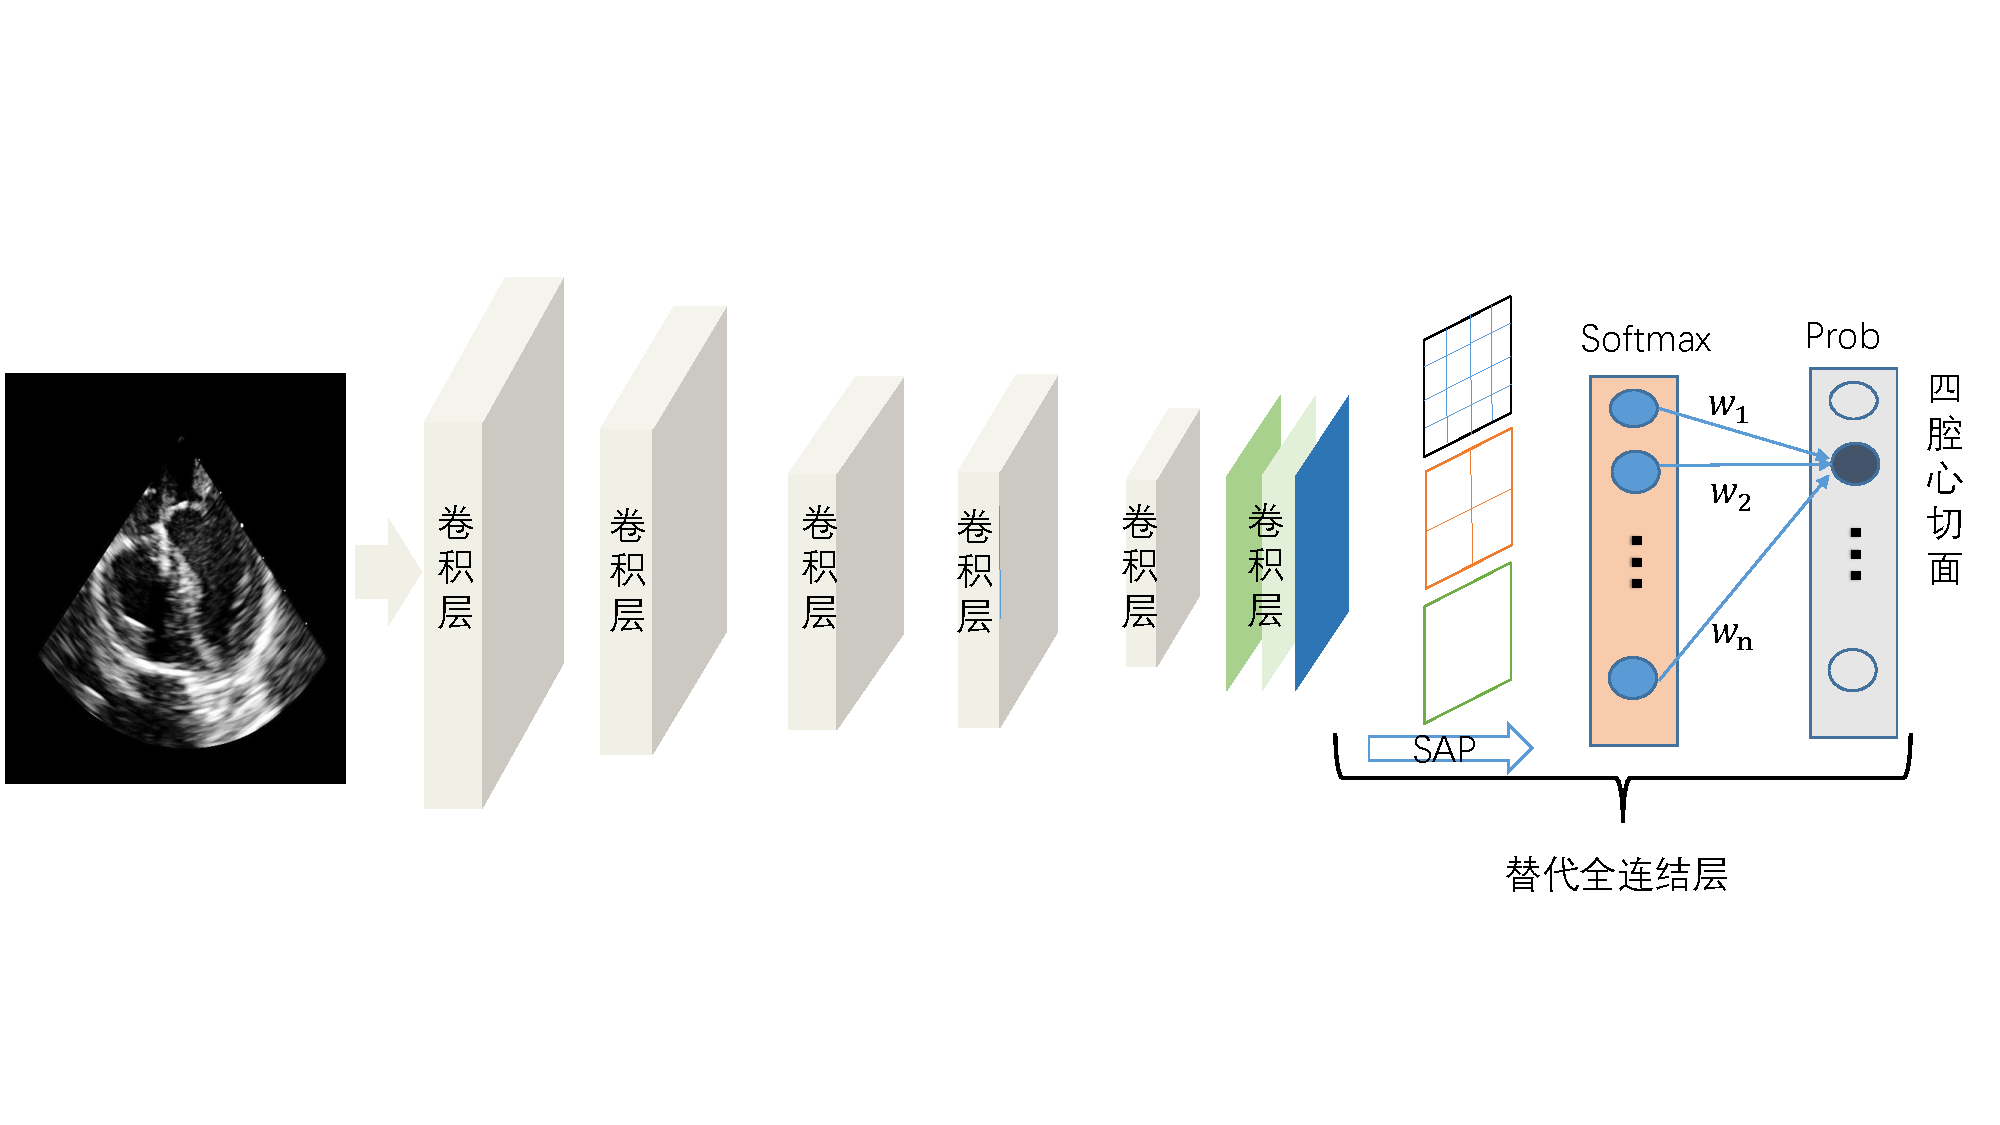
\includegraphics[trim = 30mm 0mm 30mm 0mm, clip, width=0.45\textwidth]{ch03_02}
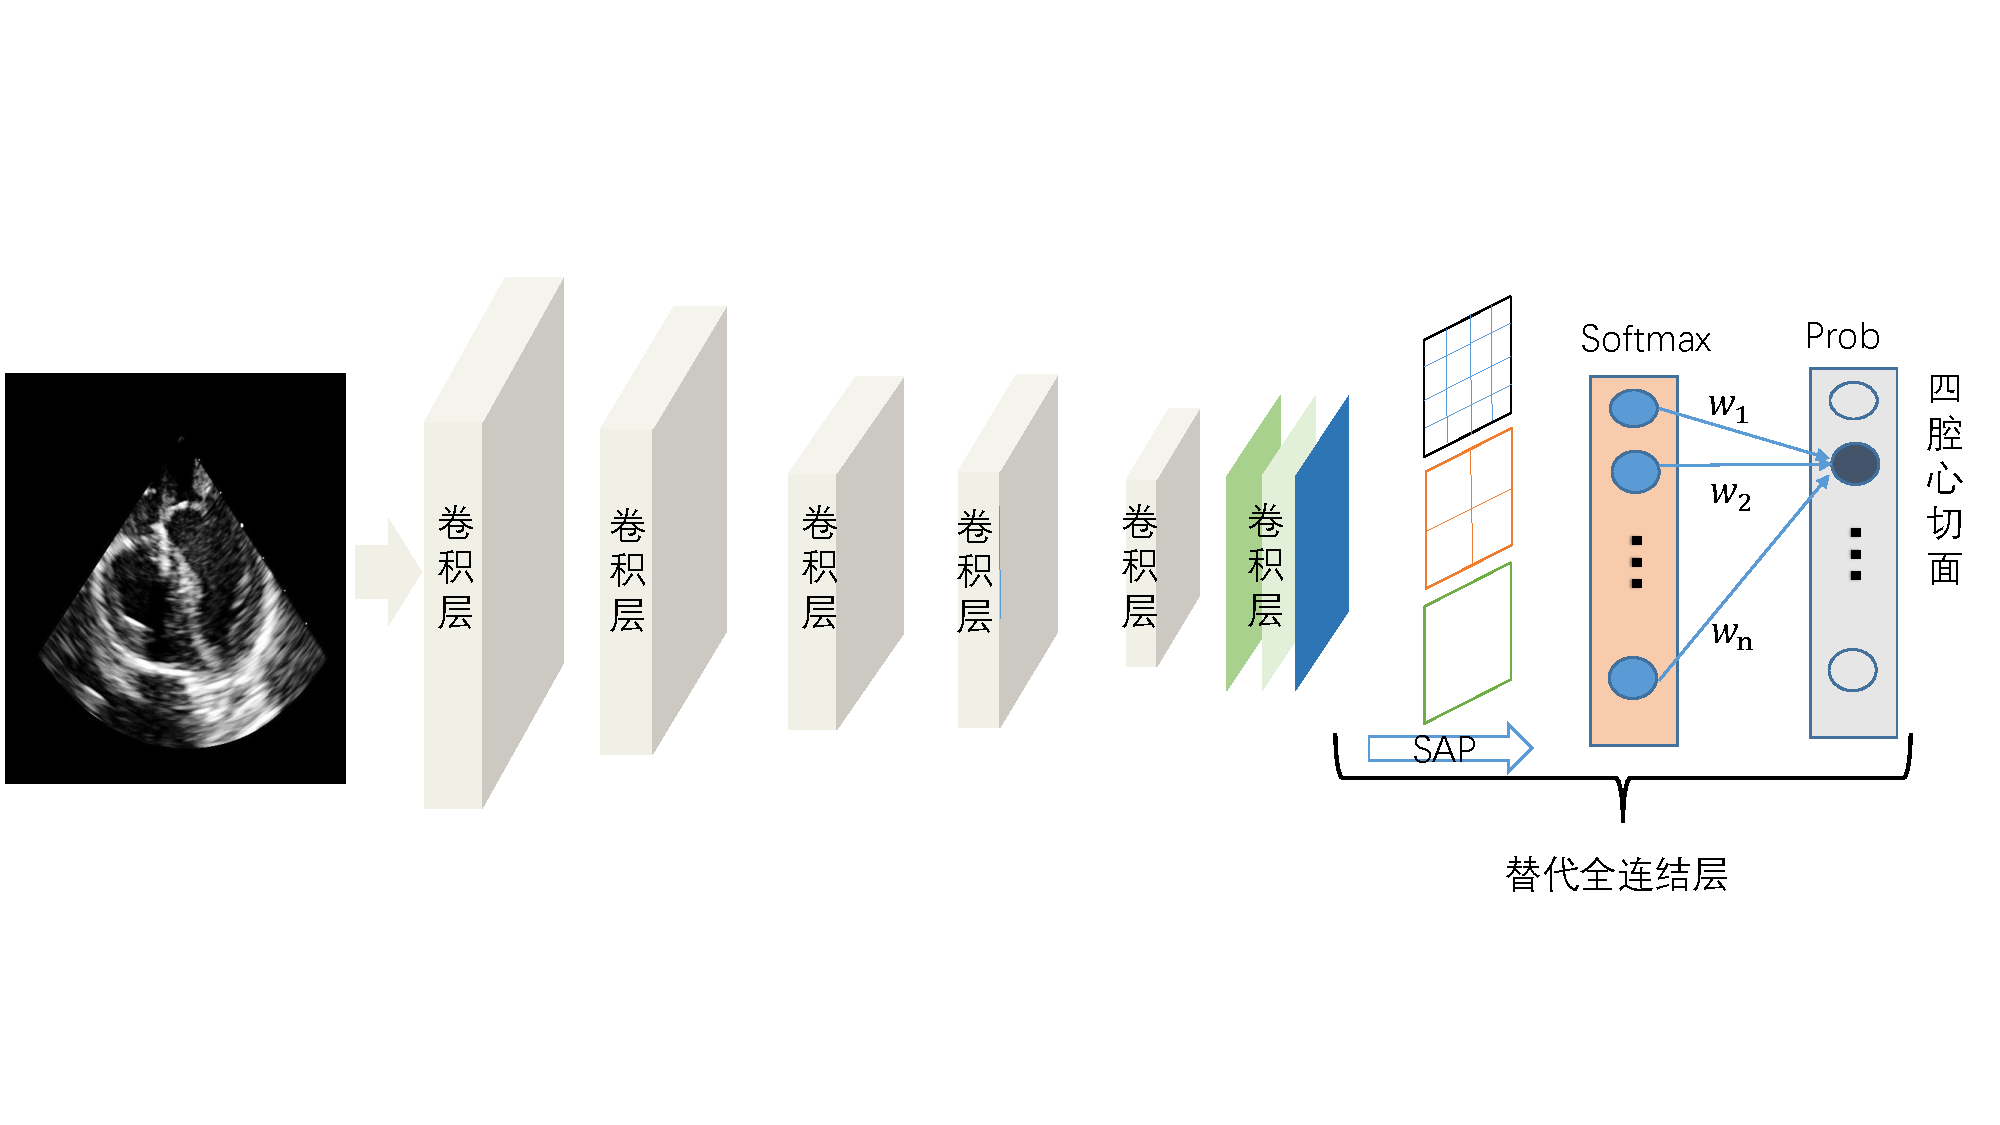
\includegraphics[width=0.85\textwidth]{ch03_02}
\caption{Deep-Echo模型结构示意图}
\label{fig:ch03_02}
\end{figure}

\subsection{空间金字塔均值池化层}

针对深度CNN模型中全连接层的两个缺点:全连接层丢失了空间信息,限制了 CNN 只能接受固定尺度的输入, 一般只能通过图像尺度归一化的方法来处理不同尺度的输入图像,且使得模型可视化变得不可解释;全连接层参数拥有大约90\%的模型参数,如AlexNet模型\citep{Krizhevsky2012}和VGG16模型\citep{Chatfield2014}中全连接层参数占全部参数分别为38M/61M和103M/138M,从而导致模型更容易过拟合\citep{Szegedy2015}。
为解决这两个问题,He等提出空间金字塔池化 (Spatial Pyramid Pooling, SPP)方法\citep{he2015spp}。 SPP通过使用多个不同大小的池化操作保证固定的特征向量输出,从而允许 CNN 接受任何尺度的输入, 增加了模型的尺度不变性, 抑制过拟合。与传统的全连接层不同,对每个特征图一整张图片进行多尺度的空间金字塔均值池化,这样每张特征图都可以得到多个尺度的输出。本文方法跟空间金字塔池化网络类似都是三个尺度的空间金字塔池化(1×1, 2×2, 4×4),其差异在于后不再接多个全连接层,同时用平均池化代替最大化池化,目的在于方便可视化模型的空间位置信息。
\subsection{微调迁移学习}

   利用深度学习进行超声心动图的标准切面识别,仍存在针对小数据量直接训练是否会出现过拟合问题;能否跨领域进行迁移学习,即在自然图像数据集上训练得到的模型能否微调应用到跨领域的超声心动图上。文献\citepns{Zhou2015}中指出,用全局平均池化代替全连接层直接随机初始化,从头开始训练模型收敛困难且分类性能下降,故对现有模型进行改造,即针对在自然图像集上预先训练得到的模型如,Alexnet模型等,变换最后的输出层为所述金字塔平均池化结构,调小学习率后在超声心动图标准切面数据上进行微调迁移学习。
训练时,由于超声心动图的特殊性,人工标注费时费力,对数据集进行扩增能降低人工标注的需求。但扩增数据需注意不能打乱标准切面图像内在的局部结构,因此对切面数据只进行水平镜像翻转和旋转。通过引入BN归一化层能减轻对Dropout的依赖,提高泛化能力,并且本文直接去掉全连接层,故并未采用Dropout技术。
迁移学习时,由于深度模型中低层的卷积核是跟人类视觉的初级细胞很类似,因此是可以直接迁移复用,高层要针对目标学习判别性信息需进行重新学习\citep{Zhou2015}。针对超声心动图的实验支持这样的结论,不同模型的分类准确率都很高,具体实验见后文实验部分。但对于计算机医学辅助诊断而言,模型怎样决策判断比分类准确率更重要。即需解释模型为什么有效和优异的泛化能力从何而来。
\subsection{类别显著激活映射图}

 前文所提模型能高效提取超声心动图标准切面的特征,对超声心动图的单扇形和双扇形标准切面都能很好的识别,甚至对互联网上随意选取的标准切面也能识别。但对模型的有效性和解释性缺乏有力分析,使得对模型决策判断的可信性产生怀疑。
针对超声心动图,采用\citepns{Zhou2015}提出可视化分析的方法,将其和空间金字塔平均池化结合。对给定图像, $f_{j}(x,y)$ 表示卷积层(x,y)位置上第j个神经元的激活值,对第j神经元的平均池化操作结果对给定类别k的得分函数S:
  \begin{equation} \label{eq:s}
     S_{k}=\sum_{j}w_{j}^{k}\sum_{x,y}f_{j}(x,y)
\end{equation}	    
其中 $w_{j}^{k}$ 是第j 个神经元和第k 类的连接权重,后接多类多元逻辑损失层,然后由公式\ref{eq:m}可得定义类别激活映射图:	
  	      \begin{equation} \label{eq:m}
     M_{k}=\sum_{j}w_{j}^{k}f_{j}(x,y)
\end{equation}
其中,$M_{k}$ 表明在空间(x,y)的激活值对该类别分类结果影响的重要性。对类别激活映射图直接双线性插值得到与原图大小相等的显著性图。本文将其和多尺度空间金字塔平均池化结合,得到对多个空间尺度的类别显著激活映射图。值得注意的是,对不同的尺度可设置不同的权重,本文采用同等权重进行融合。该图是对图像空间显著性区域的置信度判别,能辅助可视化分析深度模型的决策过程,在一定程度上解释模型可效性。

\section{实验结果和分析}
\subsection{实验数据选取和实验方法}

本文实验数据来自四川大学华西医院,为临床检查中的经食道超声心动图。所选切面视频包含单扇形和多普勒成像的双扇形两种,其中对双扇形的切面视频,仅取不包含彩色多普勒成像的切面(如图\ref{fig:ch03_03}所示)。经专业医师标注的标准切面视频中,至少包含2-3个心动周期,并依据医师建议从视频中截取包含一个心动周期的10帧图像,并经医师检验筛选后得到最终数据集。
\begin{figure}[!htbp]
\centering
%trim option's parameter order: left bottom right top
%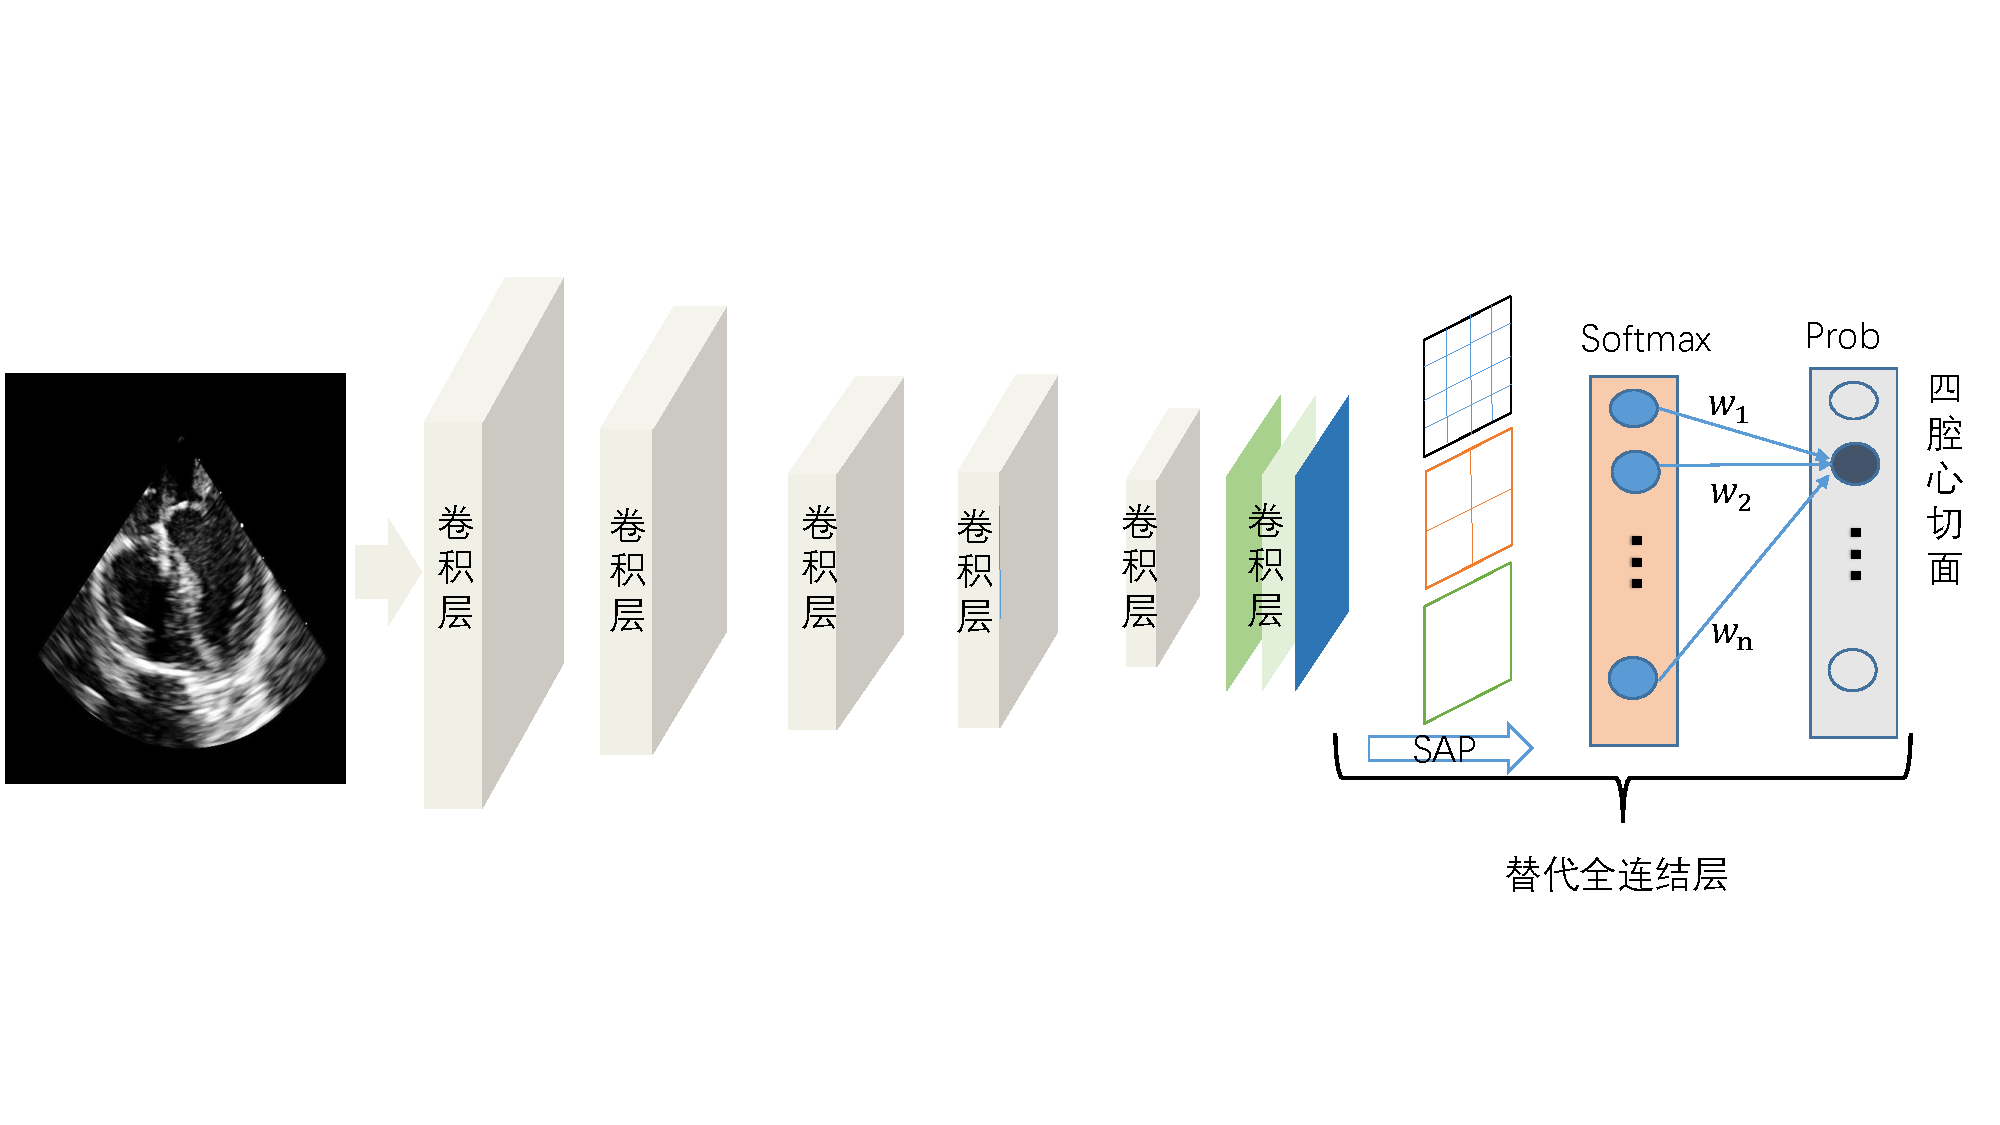
\includegraphics[trim = 30mm 0mm 30mm 0mm, clip, width=0.45\textwidth]{ch03_02}
\includegraphics[width=0.85\textwidth,height=0.4\textheight]{ch03_03}
\caption{七类标准切面超声心动图及数量分布}
\label{fig:ch03_03}
\end{figure}

试验中所用标准切面类别和数量分如布图\ref{fig:ch03_03}所示。依据探头在食管中段(ME)和经胃底(TG)的位置和角度不同,在图\ref{fig:ch03_03}中7类标准切面分别为:a为升主动脉长轴(AescLAX) ,b为主动脉瓣长轴(MEAVLAX),c为主动脉瓣短轴(MEAVSAX),d为降主动脉长轴(descLAX),e为降主动脉短轴(descSAX),f为食管中段四腔心(ME4C),g为经胃底心室短轴(TGLAX)。其中,d,e,g为单扇形切面,其余为双扇形中截取的切面。训练集(17932张)和测试集(2217张)由不同时期采集不同病人对象数据的随机划分。值得注意的是,所有数据都经过裁剪操作以隐去患者信息。
\subsection{识别实验结果和分析}

	本文在构建的超声心动图的数据集上测试分类性能。采用Caffe框架\citep{Jia2014}实现深度卷积网络结构, 预训练模型来自Caffe model zoo。使用具有Intel®Core TM i5 3.2GHz处理器和12GB内存的Tian X GPU测量所需的时间,单个切面所需的分类识别时间平均需要10毫秒,基本可满足实时识别。
为验证从自然图像训练的模型能迁移到经食道超声心动图上,输入图像归一化为256x256,网络初始学习率设为0.001,迭代一定轮数动态调整学习率大小,其他参数的设置跟原文献中训练网络结构时一致。 三种不同网络结构的深度模型微调前后在同一测试集上的准确率随着迭代次数的增加最后趋于一致,如表\ref{tab:ch03_01}所示,Scratch表示不经过微调,Finetune表示经过微调。Deep-echo模型结构跟AlexNet模型类似,是在其结构基础上去掉全连接层,用空间金字塔池化层代替,比VGG16和GoogLeNet模型的层数更少,模型结构更简单,而分类准确率却接近,表明提出方法的有效性。针对VGG16模型和Google Net模型也可同样设置,本文主要关注点不是得到分类精度最优的分类模型,故并未全部加以实验验证。
\begin{figure}[!htbp]
\centering
%trim option's parameter order: left bottom right top
%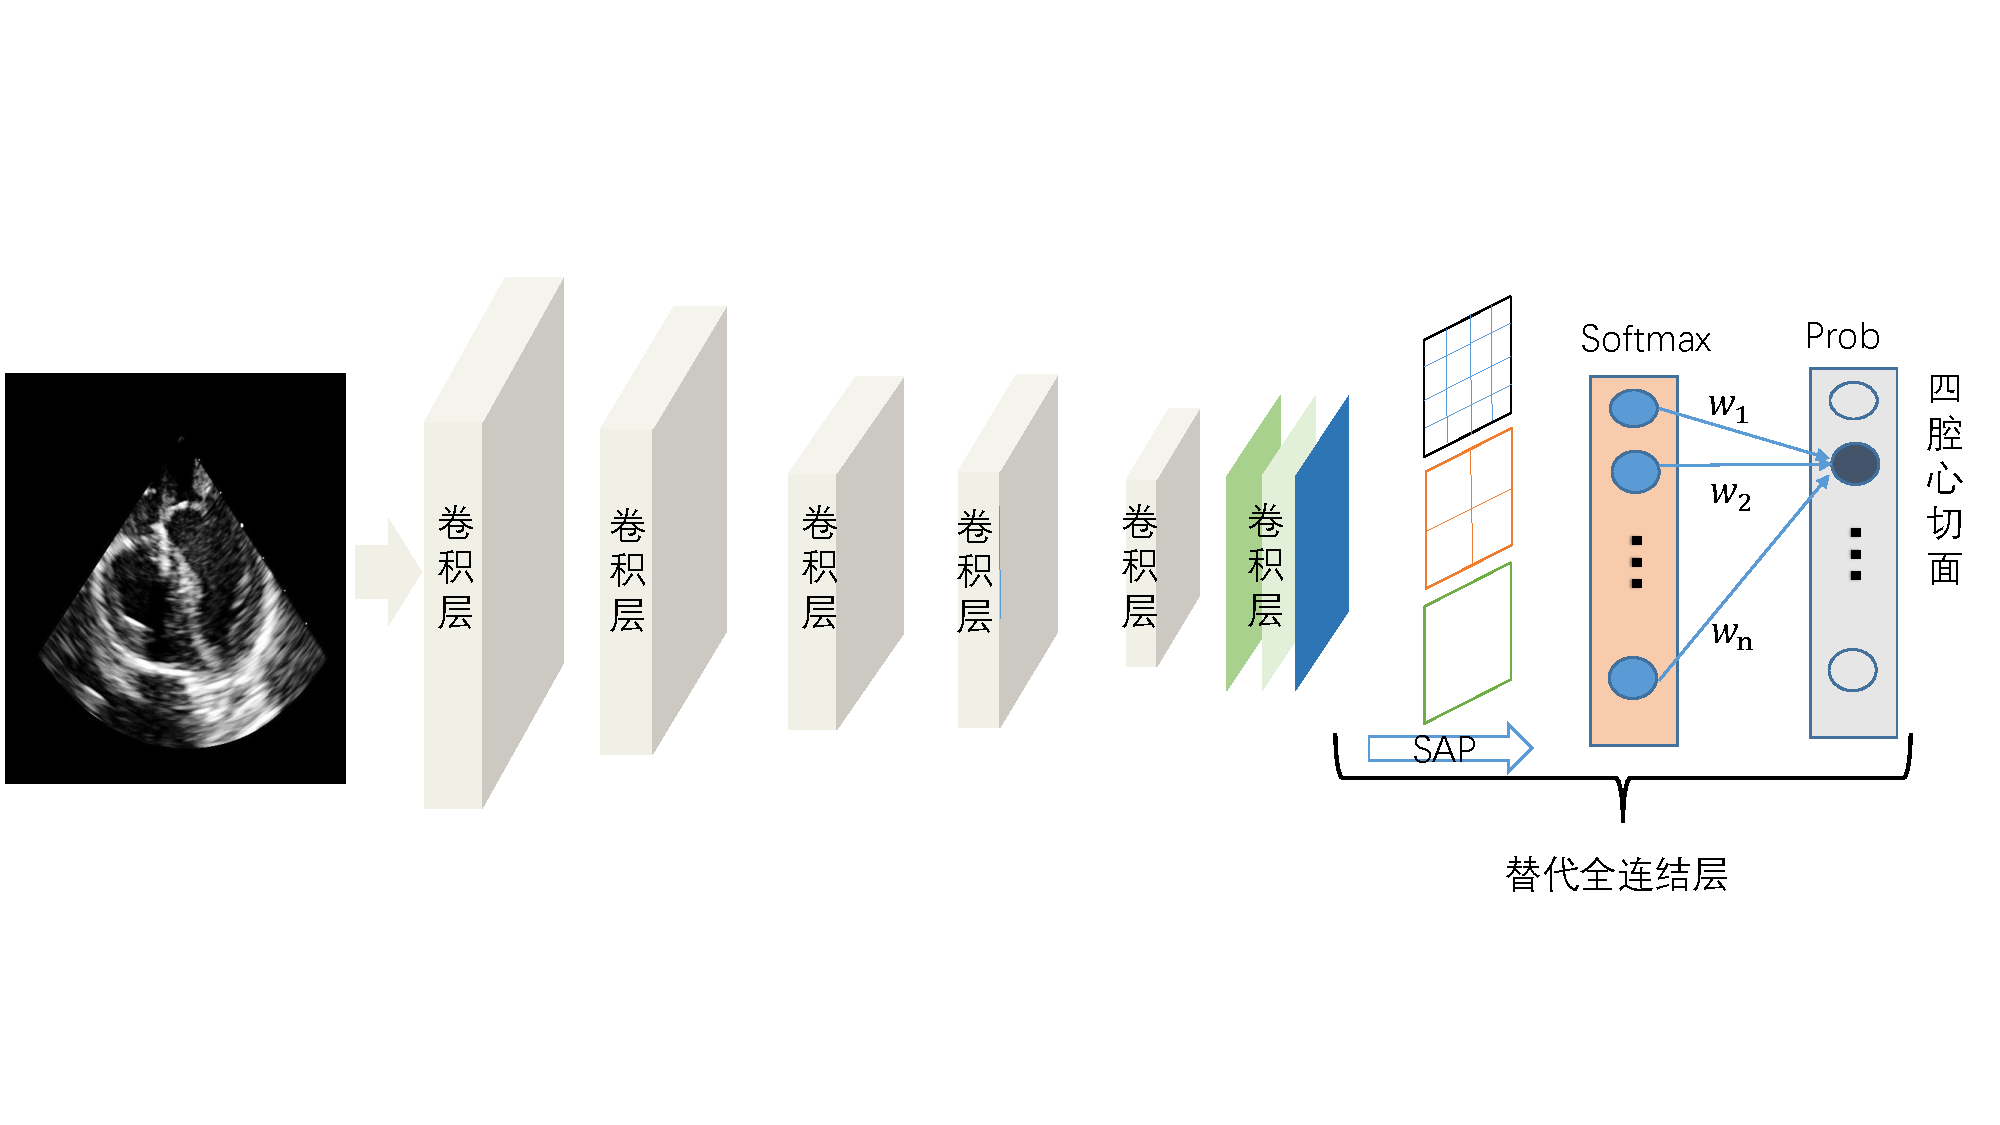
\includegraphics[trim = 30mm 0mm 30mm 0mm, clip, width=0.45\textwidth]{ch03_02}
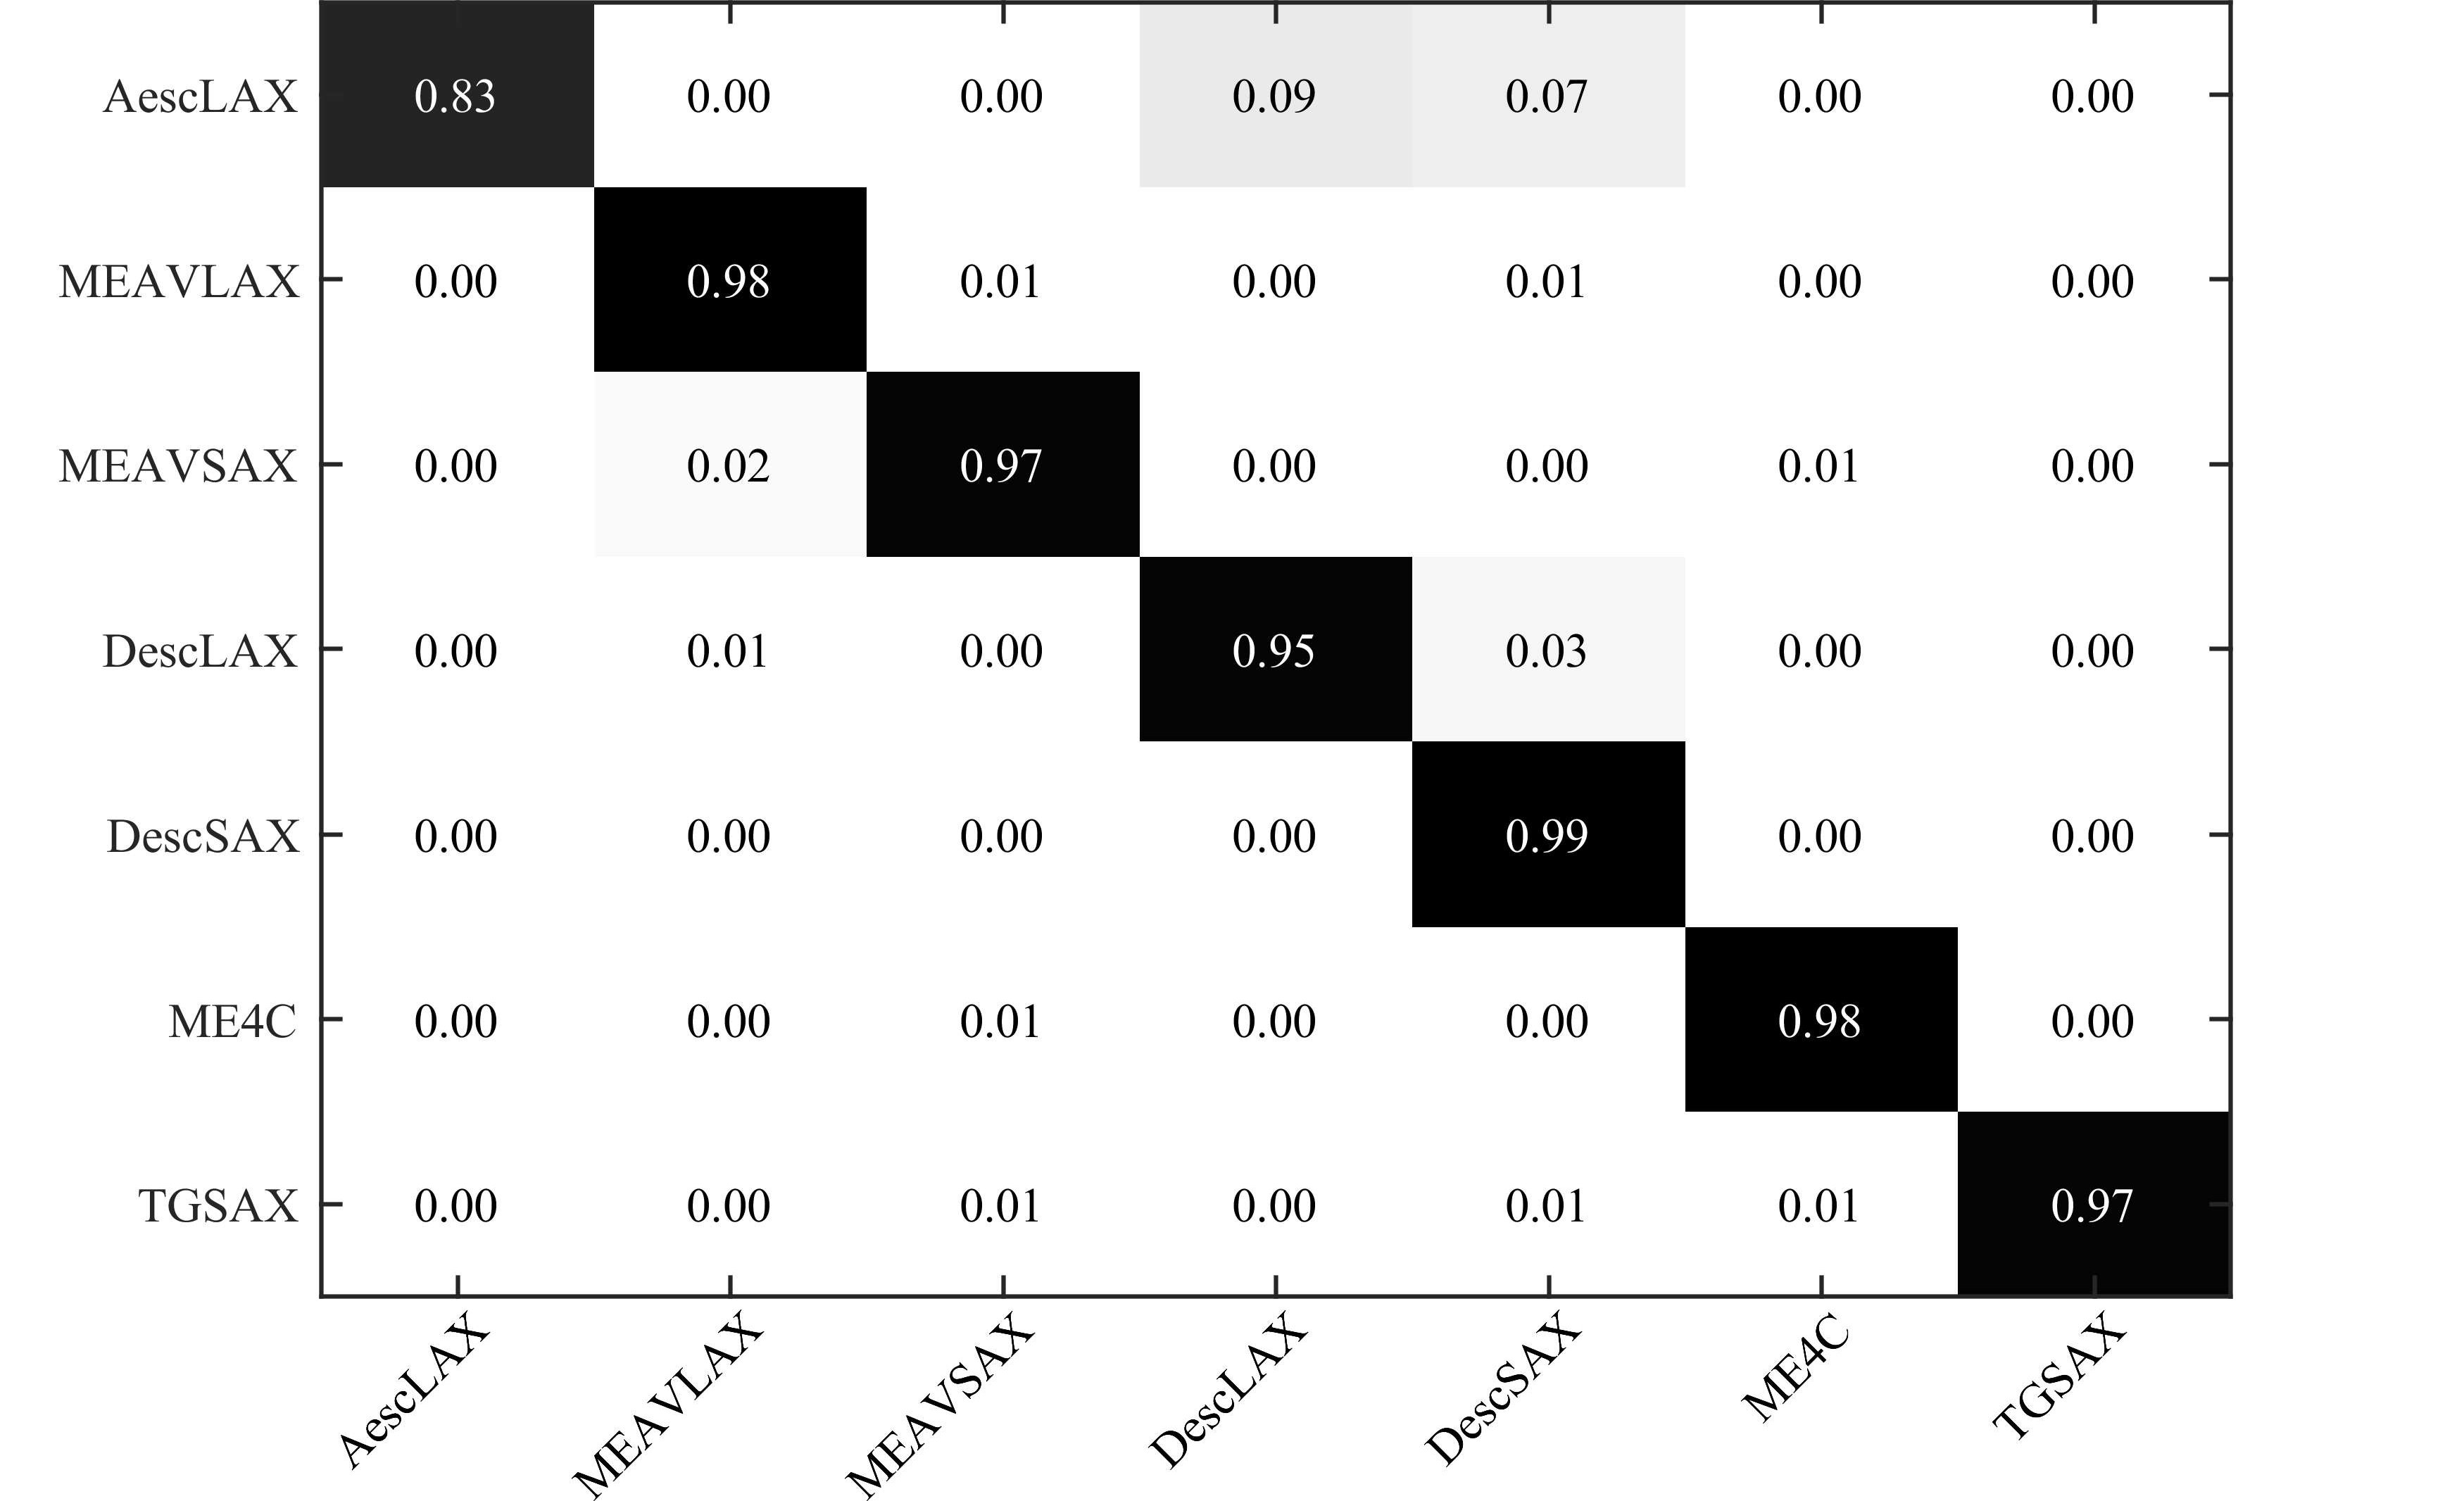
\includegraphics[width=0.85\textwidth]{ch03_04}
\caption{不同数据量的平均分类精度}
\label{fig:ch03_04}
\end{figure} 
为验证训练集数据量对深度卷积网络的影响。网络结构采用AlexNet模型结合空间金字塔池化层,在不同数据量上微调,实验结果如图\ref{fig:ch03_04}所示,数字代表每类至多的数目,随着数据量的增加,模型准确率随之提升,可知针对超声心动图标准切面识别问题,并不用构建很大的数据集进行识别,如图\ref{fig:ch03_03}中每类至多500达到的平均准确率接近使用全部训练集的结果。可推断采用微调技术,能显著减少深度模型对大数据量的依赖。
\begin{table}[!htbp]
    \centering
    \footnotesize% fontsize
    \setlength{\tabcolsep}{4pt}% column separation
    \renewcommand{\arraystretch}{1.2}%row space 
    \begin{tabular}{lcccccccc}
        \hline\hline
          \multicolumn{2}{c}{\ \ \ \ \ \ \ \ 平均分类精度比较} \\
        \cline{2-3}% partial hline from column i to column j
           \qquad  & Scratch & Finetune \\
        \hline
        AlexNet & $93.35\%$ & $93.68\%$ \\
        \hline
        VGG16 & $96.66\%$ & $96.81\%$ \\
        \hline
        GoogleNet & $97.36\%$ & $97.42\%$ \\
        \hline
        Deep-Echo & $\textbf{97.49\%}$ & $\textbf{99.12\%}$ \\
        \hline\hline
    \end{tabular}
    \caption{不同模型分类精度比较}
    \label{tab:ch03_01}
\end{table}


为了验证最优模型在不同类别的分类性能,7分类的混淆矩阵如图\ref{fig:ch03_04}所示,每行代表实际的类别标签,每列代表预测的标签。最终的平均分类精度为97.49\%。分类置信度较低的是升主动脉长轴(AescLAX),其他各类的准确率都较高。

\subsection{模型可解释性实验结果分析}
深度卷积网络能在标准切面识别问题上得到较高的分类精度,但仅从分类准确率上评价模型存在局限性。为分析模型的有效性,采用文中所述可视化方法,对迁移后的Deep-echo模型进行实验。
\begin{figure}[!htbp]
\centering
%trim option's parameter order: left bottom right top
%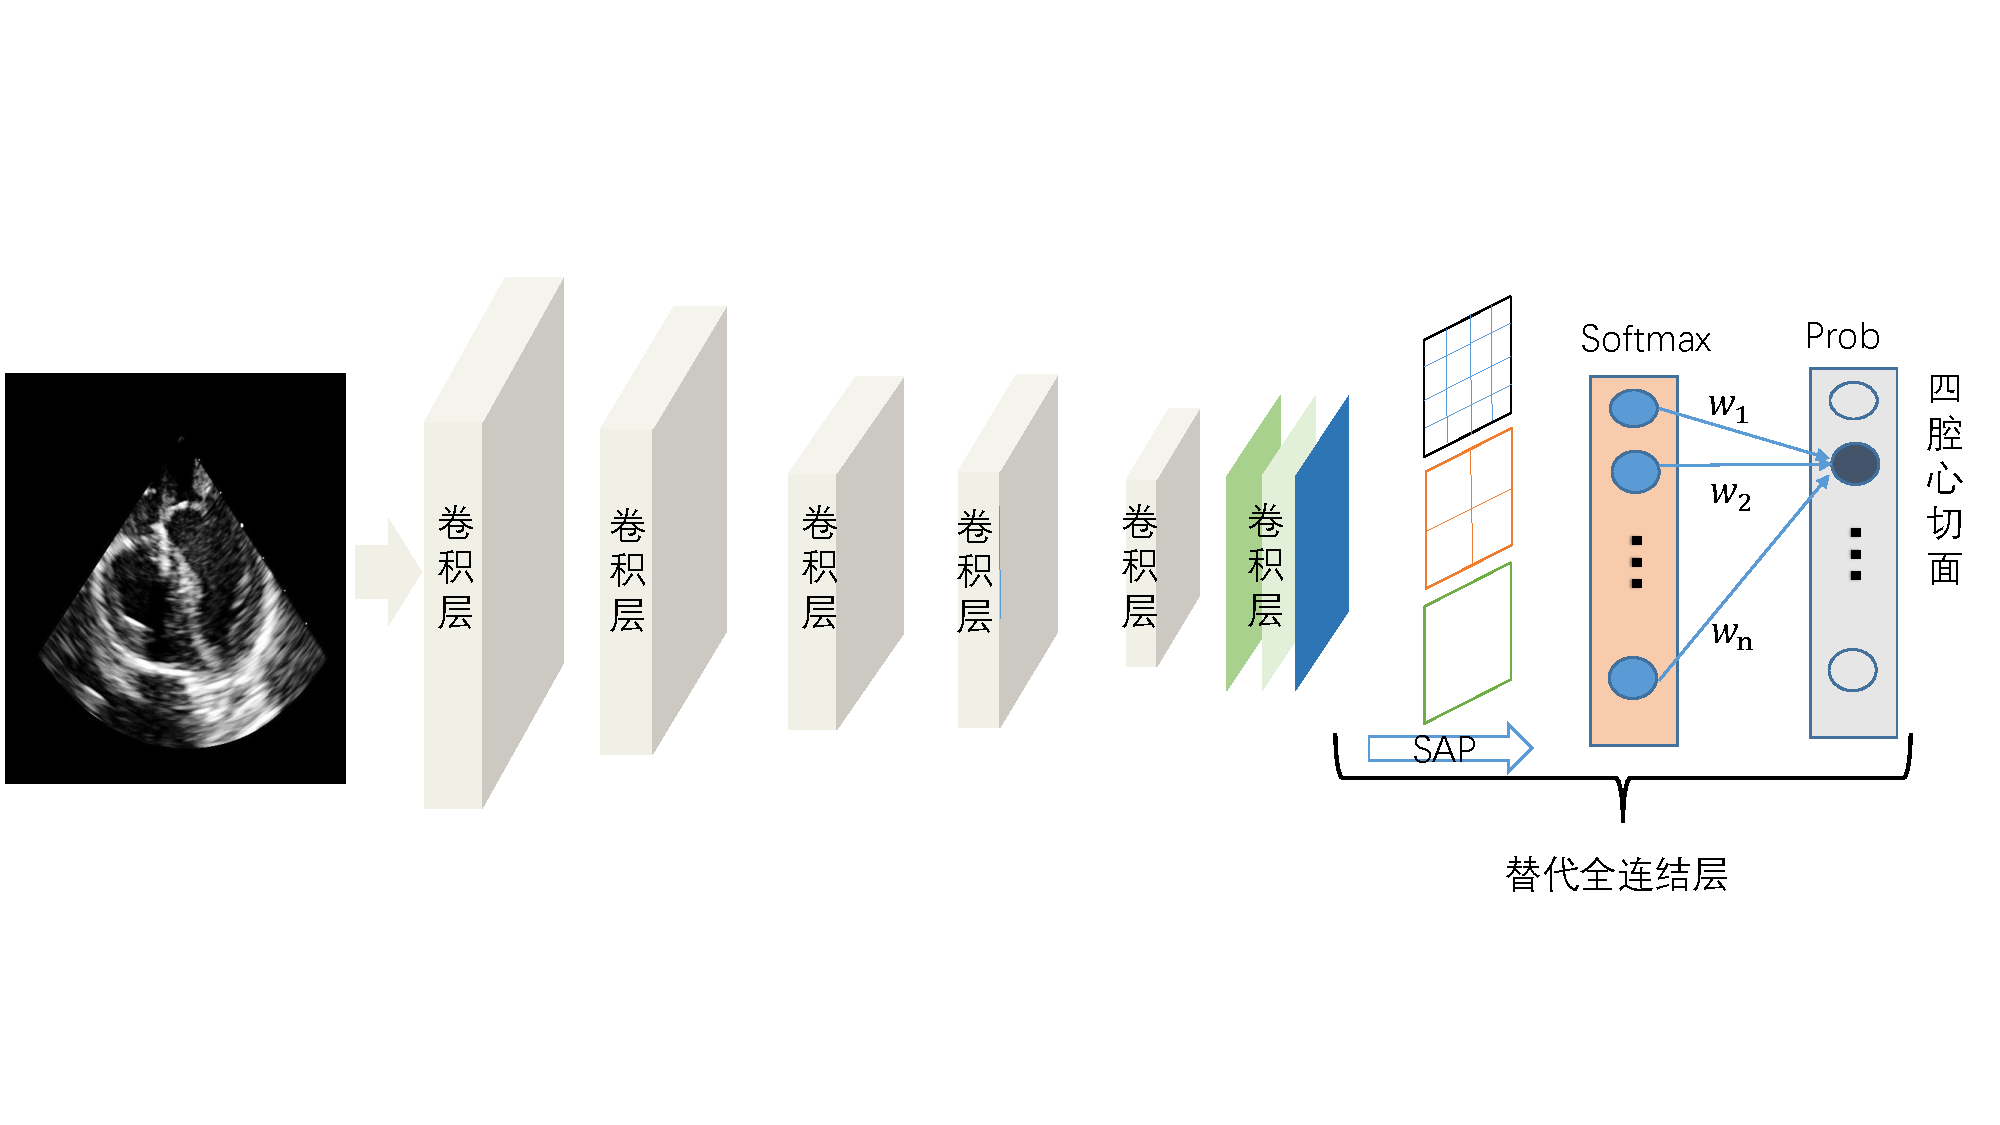
\includegraphics[scale=0.6,trim = 30mm 0mm 30mm 0mm, clip, width=0.45\textwidth]{ch03_02}
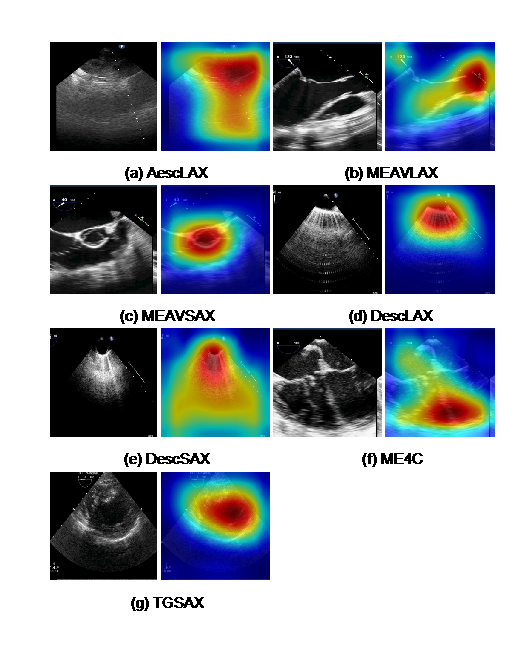
\includegraphics[width=0.85\textwidth,height=0.4\textheight]{ch03_05}
\caption{各类切面的原图和显著性热力图}
\label{fig:ch03_05}
\end{figure}  
 
实验结果如图\ref{fig:ch03_05}各类切面的原图和显著性热力图所示,图中为各类切面和对应的类别显著性热力图。类别显著性图中的颜色从蓝到红,表示原图像素中对分类结果影响的重要性是从轻到重。图中结果能很好的解释模型的有效性,并且跟专业医师的判断一致,如图\ref{fig:ch03_05}c中显著性热力图红色区域图定位到图中的圆圈;图\ref{fig:ch03_05}d中定位到的干涉条纹;图\ref{fig:ch03_05}f定位到左心室和右心室的边界等;都跟医师的决策判断依据是一致的。
\begin{figure}[!htbp]
\centering
%trim option's parameter order: left bottom right top
%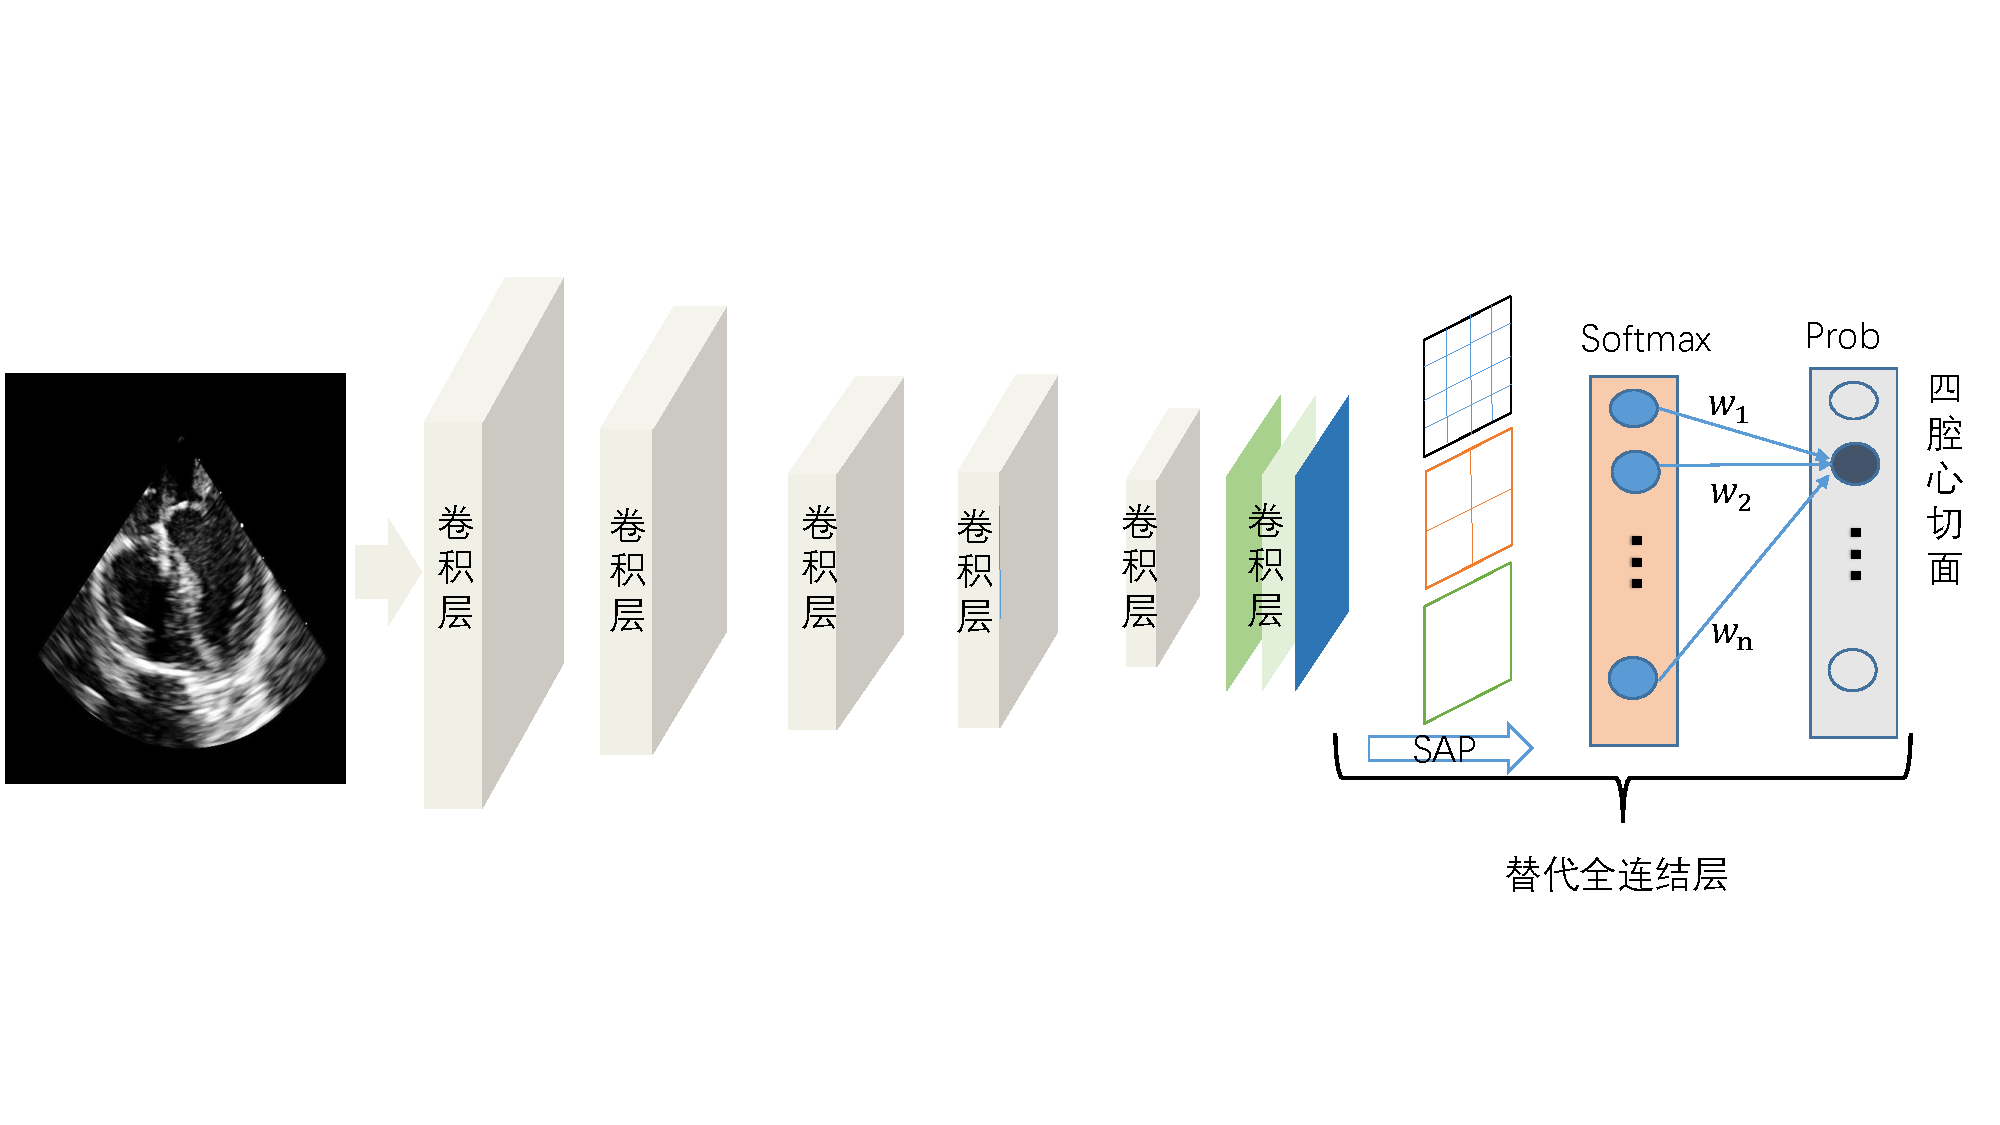
\includegraphics[scale=0.6,trim = 30mm 0mm 30mm 0mm, clip, width=0.45\textwidth]{ch03_02}
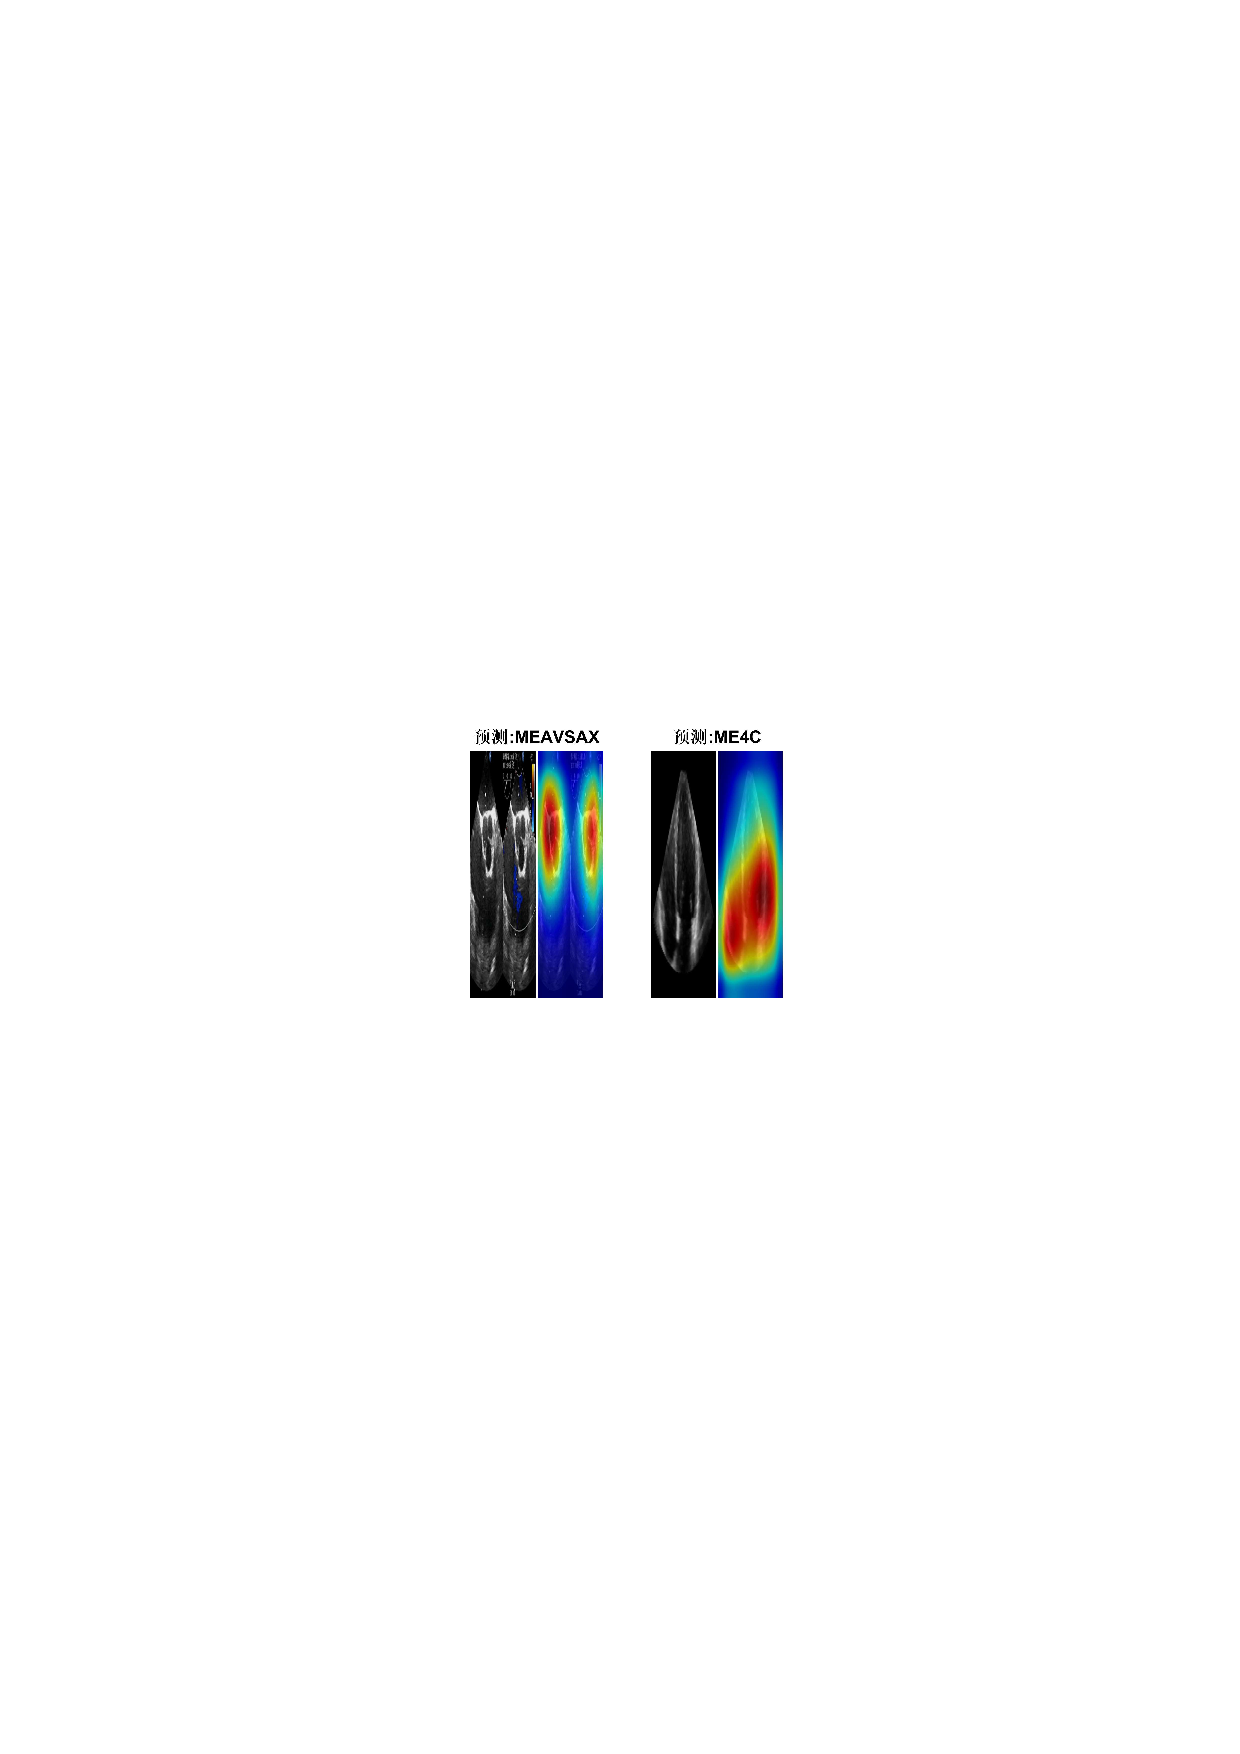
\includegraphics[width=0.85\textwidth,height=0.15\textheight]{ch03_06}
\caption{深度模型泛化性能可视化分析}
\label{fig:ch03_06}
\end{figure}  
  
深度模型泛化性能可视化结果如图\ref{fig:ch03_06}所示,原图像分别是带彩色多普勒的双扇形切面(图\ref{fig:ch03_06}a)和经胸的四腔心切面(图\ref{fig:ch03_06}b),这两个图是跟数据集中的经食道超声心动图差异较大,说明深度卷积网络模型确实能对标准切面进行语义分类, 表明模型确实能提取到高层语义的特征, 深度卷积网络泛化能力优异。图7中可视化结果也能很好的解释模型的有效性,如图\ref{fig:ch03_06}中显著性热力图红色区域图定位到图中的圆圈,也是医师认定该切面的关键性结构,图\ref{fig:ch03_06}b定位到左心室和右心室的边界等,都跟医师的决策判断依据是一致的。并且该方法也能作为判断学习模型是否有效的根据,不经过微调的模型虽然能得到较高的分类准确度,并不能得到类似的显著性热力图。

\section{本章小结}

本文提出了一种基于深度卷积神经网络的超声心动图标准切面自动识别方法,利用所述全局空间金字塔均值池化方法进行微调迁移学习,实验结果表明该方法识别准确率高,并实验分析了数据规模对模型分类精度的影响,结果表明基于深度卷积网络的识别方法应成为超声心动图自动识别的基准方法,接下来会探索更精细类别分类问题,如舒张末期和收缩末期标准切面的识别等。可视化深度模型的实验,对模型的可解释性和有效性进行了分析,推断深度模型的优异的分类性能和泛化能力的原因是可以对类别显著性区域进行判别,采用的可视化方法是对网络模型整体的理解,具体各层特征怎么耦合成语义信息仍需进一步探索。





\chapter{空间金字塔分解的深度可视化方法}
\label{chap:visualization}

 提出了一种基于深度卷积神经网络自动识别超声心动图标准切面的方法,并可视化分析了深度模型的有效性。该算法针对网络全连接层占有模型大部分参数的缺点,引入空间金字塔均值池化替代全连接层,获得更多的空间结构信息,并大大减少模型参数、降低过拟合风险,通过类别显著性区域将类似注意力机制引入模型可视化过程。通过超声心动图标准切面的识别问题案例,试着对深度卷积神经网络模型的鲁棒性和有效性进行了解释。在超声心动图上的可视化分析实验表明,通过改进方法的深度模型的识别决策依据,同医师辨别分类超声心动图标准切面的依据一致,表明了方法的有效性和实用性。

\section{引言}

以深度卷积神经网络(Convolutional Neural Network ,CNN)为代表的深度学习对计算机视觉和机器学习领域产生了深远影响。但是完全理解深度学习模型的内在工作原理,设计高性能的深度网络结构还是很困难的,一直以来人们普遍将其内部工作原理看成一个“黑箱”,这是由于深度CNN存在海量参数,多次迭代更新生成输入输出之间相当不连续和非线性的映射函数;以及对参数的初始状态敏感,存在很多局部最优点。探究CNN的运行机制,核心在于它究竟自动提取什么样的特征,经过卷积层、池化层,特征都是分布式表达的,每个特征反映在原图上都会有重叠,故希望建立特征图与原图像之间的联系,即深度可视化。该技术试图寻找深度模型所提取各层特征较好的定性解释,并在设计开发新网络结构方面扮演重要角色。


目前针对CNN可视化的研究,主要集中在如何理解CNN从海量数据中自动学习到的,能反映图像本质的分层特征表达,即获得网络中隐藏层神经元与人类可解释性概念之间的联系。最直接的方法是展示学习得到的卷积核和相应的特征图,但除了首层卷积核和特征图有直观的解释外,其余各层并没有可解释性。从信号处理的角度看,基于CNN高层特征的分类器在输入域,需要较大感知野,才能对以由低频为主的输入图像进行多层非线性响应,并对小的输入改变产生平滑不变输出。同时,由于经过非线性激活函数变换和池化,引入空间不变性获得更好识别性能的同时,也对可视化带来新的挑战。


深度可视化技术可以简单分为三类:基于梯度更新的方法\citep{Erhan2009,simonyan14deep,Lenc2015,Szegedy2013a,JasonYosinski2015,Nguyen2016a,Nguyen2016b};基于特征重建的方法\citep{Zeiler2014,Brox,Mahendran2015d,Mahendran2015}];基于相关性的方法\citep{Cao2015,Bach2016}。基于网络梯度更新的思想是由Erhan等\citep{Erhan2009}引入,固定模型参数通过梯度更新改变输入值,最大化激活单一神经元或标签类别概率。激活最大化生成的非自然图像还可以是网络模型的对抗样本\citep{Goodfellow2014}。Simonyan等\citep{simonyan14deep,Lenc2015,Szegedy2013a}通过梯度上升方法迭代寻找使得最大化激活CNN某个或某些特定的神经元的最优图像,其假设神经元对像素的梯度描述了当前像素的改变能影响分类结果的强度。文献\citepns{simonyan14deep}引入L2正则化先验(或称权重衰减),改进可视化效果。Yosinski等\citep{JasonYosinski2015}进一步提出高斯模糊正则化、梯度剪切等技术,其中梯度剪切指的是每次只更新对分类最有利的一部分梯度,改善生成图像质量。文献\citepns{Lenc2015,Nguyen2016b}考虑神经元的多面性和利用生成网络作为自然图像的先验来合成更自然的图像。
Zeiler等\citep{Zeiler2014}提出利用反卷积网络,利用反向传播重构各层特征到像素空间的映射,并用于指导设计调优网络结构,提高分类识别精度。在反卷积过程中利用翻转原卷积核近似作为反卷积核,针对特定特征图在训练集上重新训练。Dosovitskiy等\citep{Brox}提出通过学习‘上’卷积网络来重建CNN各层的特征,指出结合强先验,即使用于分类的高层激活特征也包含颜色和轮廓信息。Mahendran等\citep{Mahendran2015d,Mahendran2015}通过对学习到的每层特征表达进行反编码重建,提出利用全变分正则化和自然图像先验,并将L2范数正则化推广到p范数正则化,得到较优的可视化效果。


本文主要关注前两种方法中的正则化技术,基于相关性分解方法请参考文献\citepns{Bach2016}。受文献\citep{Huang2017c,Denton2015}启发,把用于图像生成的拉普拉斯金字塔,进一步扩展成空间金字塔分解方法,并引入显著性激活图技术进一步改进深度CNN的可视化效果。
\section{ 可视化方法的数学模型}

激活最大化和特征表达反编码重建均是针对已经训练好的模型,对给定输入$x_{i}\in R^{C\times H\times W}$ ,其中C为颜色通道数,H,W为图像高和宽。CNN模型可抽象为函数$\phi$:$R^{C\times H\times W}\rightarrow R^d$ ,其第i个神经元的激活值为$\phi _{i}(x)$ ,对给定图像$x_{0}$ 的特征编码$\phi _{0}=\phi (x_{0})$ ,定义参数$\theta$ 的正则化项$R_{\theta}(x)$ ,寻找使得能量泛函最小化的初始输入$x^*$ ,其数学模型为
\begin{equation} \label{eq:ch04_01}
     x^*=\underset{x}{argmin} (l(\phi (x),\phi _{0})) + \lambda R_\theta(x))
\end{equation}
其中, $l$损失比较的是$\phi (x)$ 和目标$\phi_{0}$ 的差异,选择不同的损失函数定义不同的可视化方法。但该优化通常是一个非凸优化问题,通常采用梯度下降法去寻找局部最优值为
\begin{equation} \label{eq:ch04_02}
     x \leftarrow x+ \alpha \frac{\partial \phi _{i}(x)}{\partial x}
\end{equation}
激活最大化方法是文献\citepns{Erhan2009}中提出针对深度架构中任意层中的任意神经元所提取的特征,寻找使一个给定的隐含层单元的响应值$\phi _{0}\in R^d$ 最大的输入模式,可由内积形式定义$l$ 损失为
\begin{equation} \label{eq:ch04_03}
     l(\phi (x),\phi_{0}) =-<\phi (x),\phi _{0}>
\end{equation}
  式中$\phi_{0}$ 需人工指定,最大化激活的目标可以是全连接层的特征向量,也可以是卷积层某一通道的某一神经元的激活值。
特征表达的反编码重建,通过最小化给定特征向量与重建目标图像特征向量间的 损失,一般采用欧式距离来衡量损失误差,定义如下 
\begin{equation} \label{eq:ch04_04}
     l(\phi (x),\phi _{0}) = \frac{\parallel\phi (x)-\phi _{0} \parallel^2 }{\parallel \phi _{0} \parallel^2 }
\end{equation} 
但也可利用其它距离度量函数来评价损失。

\section{梯度更新的可视化方法}
 
   用于分类的深度CNN提取高层语义信息的同时,丢失了大量低层结构信息。由于首层卷积核大都类似Gabor滤波器,导致梯度更新可视化生成图像中包含许多高频信息,虽然能产生大的响应激活值,但对可视化来说导致生成的图像是不自然的。还由于网络模型的线性操作(如卷积)导致对抗样本\citep{Goodfellow2014}的存在,为得到更类似真实自然图像的可视化结果,需在优化目标函数中引入正则化作为先验。
\subsection{$p$ 范数正则化方法} 

   对图像来说,像素大小需在一定范围内,直接最大化激活类别概率,生成图像类似随机噪声图像。文献\citepns{simonyan14deep}通常引入L2范数正则化,惩罚过大和过小的极端值,其公式为$R_{\theta}(x)=\parallel x \parallel _{2}^{2}$ 。在文献\citep{Mahendran2015}中将其扩展到彩色图像RGB通道空间中的$p$范数正则化为
\begin{equation} \label{eq:ch04_05}
       R_{\theta}(x)= \frac{1}{HWC^p}\sum_{h=1}^{H}\sum_{w=1}^{W}(\sum_{c=1}^{C}x(x,w,c)^2)^{\frac{p}{2}}
\end{equation}
式中h,w表示图像的行和列大小,c表示颜色通道数,对比发现,文献\citepns{simonyan14deep}提出的L2正则化是忽视各颜色通道的差异的,正则化的力度可通过缩放常量p进行控制,即使得图像像素值大小保持在合适的范围内。
\subsection{高斯模糊和TV变分}

基于梯度更新可视化方法,引入高斯滤波器主动惩罚高频信息\citep{JasonYosinski2015},高斯模糊核半径大小由高斯函数的标准差控制,可随迭代次数动态调整模糊核大小。


全变分\citep{Mahendran2015}(Total Variance,TV)跟高斯模糊类似,鼓励可视化生成分片的常量块区域,对离散图像全变分操作可由有限差分来近似求解为    \begin{equation} \label{eq:ch04_06}
       R_{TV}(x)= \frac{1}{HWC^\beta}\sum _{hwc}((x(h,w+1,c)-x(h,w,c))^2+(x(h+1,w,c)-x(h,w,c))^2)^{\frac{\beta}{2}}
\end{equation}
式中 $\beta =1$,但其在可视化过程中,在图像的平坦区域并不存在边缘,全变分操作仍沿着边缘方向扩散就会导致出现虚假的边缘,会引入所谓的“阶梯效应”现象。 $\beta<1$时结合超拉普拉斯先验\citep{Krishnan2009}能更好匹配自然图像的梯度统计分布,但对可视化来说反而使得可视化更困难。文献\citepns{Mahendran2015}实际实验表明,跟高斯模糊核一样,需随迭代次数动态调整$\beta$ 大小。
\subsection{基于数据统计先验}

	由于常规可视化方法并没有对颜色分布进行建模,文献\citep{Lenc2015}提出通过引入外部自然图像数据,计算图像色块先验为
\begin{equation} \label{eq:ch04_07}
       R_{\theta}(x)= \sum_{p}\parallel x_{p}-D_{p}\parallel _{2}^{2}
\end{equation}
式中$p$为块索引,$x_{p}$ 表示稠密采样的归一化图像块, $D_{p}$表示自然图像块数据库中距离$x_{p}$ 最近图像块。该方法跟文献\citep{Huang2017c}中利用参考图像“指导”人脸图像嵌入重建类似。并且基于数据的统计先验可进一步扩展,引入生成对抗网络,利用生成网络主动生成自然图像先验\citep{Nguyen2016a}。

 
 
\section{空间金字塔分解}
 
前文介绍的正则化先验主动限制图像空间中高频率和高振幅信息,生成的可视化图像存在如下问题:1)彩色图像的颜色分布仍是不自然的。2)生成的图像中包含可识别类别对象的多个重复成分,并且这些部件不能组合成完整的有意义整体。3)缺乏令人可信的低频细节,存在棋盘效应,只是形似。针对这些问题提出利用空间金字塔分解,主动提升低频信息和调控高频信息以改善生成图像的可视化效果。

\subsection{高斯和拉普拉斯金字塔分解}
 
拉普拉斯金字塔(Laplacian Pyramid,LP)\citep{Burt1983}是由一系列包含带通滤波器在尺度可变的图像上加低频残差组成的。首先通过高斯平滑和亚采样获得多尺度图像,即第K层图像通过高斯模糊、下采样就可获得K+1层,反复迭代多次构建高斯金字塔(Gaussian Pyramid,GP)。用高斯金字塔的K层图像减去其第K+1层图像上采样并高斯卷积之后的预测图像,得到一系列的差值图像即为拉普拉斯金字塔分解图像。
拉普拉斯金字塔分解过程(见图1所示)包括4个步骤: 1)高斯平滑 ;2)降采样(减小尺寸); 3)上采样并高斯卷积(图中expand操作); 4)带通滤波(图像相减)  。拉普拉斯金字塔突出图像中的低频分量,拉普拉斯金字塔分解的目的是将源图像分解到不同的空间频带上。
\begin{figure}[!htbp]
\centering
%trim option's parameter order: left bottom right top
%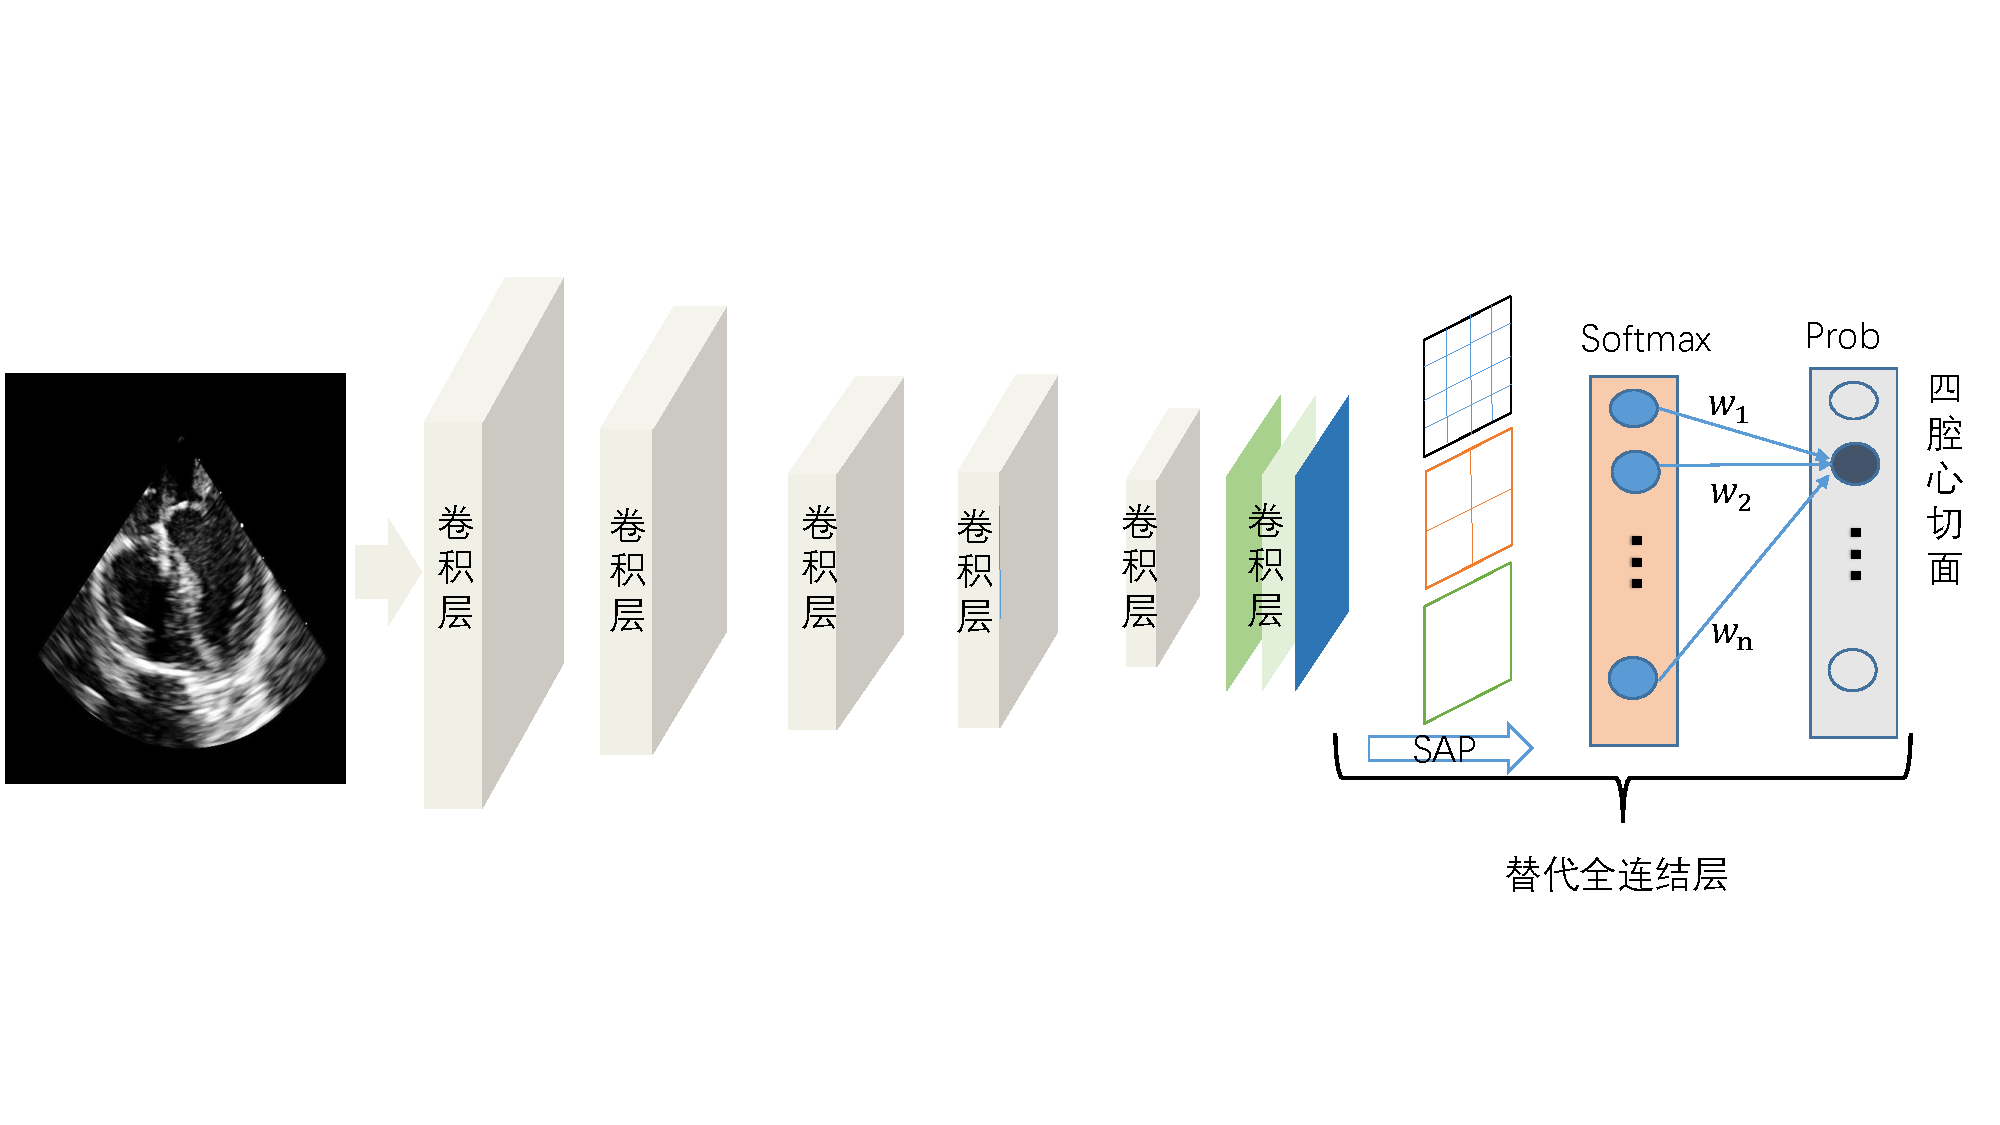
\includegraphics[trim = 30mm 0mm 30mm 0mm, clip, width=0.45\textwidth]{ch03_02}
\includegraphics[width=0.85\textwidth]{ch04_01}
\caption{高斯和拉普拉斯金字塔}
\label{fig:ch04_01}
\end{figure}

	由于自然图像统计特性中的尺度不变性,也称为$1/f$法则\citep{VanderSchaaf1996a},即自然图像集$I(f_{x},f_{y})$ 的平均傅里叶功谱服从$I~(f_{x},f_{y})^2$ 。在激活最大化可视化深度CNN模型过程中利用提出的高斯和拉普拉斯空间金字塔分解,调整生成梯度图像包含的频谱分量大小。其中空间金字塔分解正则化项为
\begin{equation} \label{eq:ch04_08}
       r_{\theta}(x)= \sum_{k=1}^{K}[LP_{k}+GP_{k}]
\end{equation}
式中k代表构建$k$层金字塔分解,本文实验$k$选取为4。 $LP_{k}$为第$k$层的拉普拉斯金字塔分量,$GP_{k}$ 为第$k$层的高斯金字塔分量。 


\subsection{梯度归一化}
  
	基于梯度更新的可视化方法,由于原输入空间中高低频分量混杂在一起,对原输入图像相应的更新梯度进行归一化操作能得到较好可视化效果,即对输入图像每次迭代更新的梯度 ,则提出梯度归一化操作:   
\begin{equation} \label{eq:ch04_09}
       g \rightarrow \frac{g}{g.std()+\delta}
\end{equation} 
式中 $\delta$为非负小常量,std表示梯度矩阵的方差。该梯度中心归一化技术,可以减少产生重复的对象碎片的倾向,而倾向于产生一个相对完整对象。梯度归一化的引入同批归一化(Batch Normalization)思想类似,校正CNN网络非线性变换引起的“偏移”,该方法也侧面验证最新提出的分层归一化\citep{Ioffe2014}的有效性。
\subsection{类别激活图限制可视化区域}
根据文献\citepns{Zhou2015}提出的类别激活图技术,假设$f_{j}(x,y)$  表示最后的卷积层空间$(x,y)$位置上第$j$ 个神经元的激活值,则对$j$ 神经元的全局平均池化操作结果对给定类别$k$的得分函数$S_{k}$:
\begin{equation} \label{eq:ch04_10}
      S_{k}=\sum _{j} w_{j}^{k} \sum _{x,y}f_{j}(x,y)
\end{equation}
式中 $w_{j}^{k}$ 是第$j$ 个神经元和第 k类的连接权重。根据文献\citepns{Zhou2015},由式\ref{eq:ch04_10} 可得定义类别激活图$M_{k}$ 为	
\begin{equation} \label{eq:ch04_11}
      M_{k}=\sum _{j} w_{j}^{k}f_{j}(x,y)
\end{equation}
式中$M_{k}$ 表明在空间(x,y)位置的激活值对分类结果影响的重要性。对类别激活映射图直接双线性插值得到与原输入图像大小相等的显著性图。本文利用显著性激活图作为梯度更新的权重因子,即输入变为原始输入图像与类别激活图的加权乘积。动机是要求网络梯度更新保持在类别显著性区域内,压制无关背景信息的生成。具体详情请参见第四章实验部分。
\subsection{优化方法}

深度CNN模型优化策略的核心是随机梯度下降法,常用方法是带动量的随机梯度下降法为:
\begin{equation} \label{eq:ch04_12}
      V_{t}=\mu V_{t-1} -\alpha *\bigtriangledown {f(x_{i})}
\end{equation}          
\begin{equation} \label{eq:ch04_13}
     x_{t+1}=x_{t}+V_{t}
\end{equation}       
式中$\mu$ 为动量因子表示保持原更新方向的大小,一般选取0.9, $x_{t}$为在t时刻待更新的梯度,$\alpha$ 为学习率;文献\citep{Mahendran2015d,Mahendran2015} 采用自适应梯度(Adaptive Gradient,AdaGrad)\citep{Duchi2011}的变种算法,根据历史梯度信息自适应调整学习率。同时文献\citepns{Gatys2015a}采用的二阶优化算法针对纹理和艺术风格重建问题,得到比用基于一阶随机梯度下降算法更优的可视化效果。但本文通过实验对比发现对各种优化方法对生成图像质量影响不大,从简选择带动量的随机梯度优化方法。
\section{实验结果分析和讨论}
 
基于梯度更新的可视化方法主要用于激活最大化和特征重建,但文献\citepns{He2016}指出用随机未训练的CNN模型也能较好重建原图像,表明特征编码重建不能很好解释训练得到CNN模型的内在工作机理。故本文实验主要关注在对ImageNet公开数据集上预先训练得到的分类模型进行激活最大化可视化实验。
\subsubsection{不同深度模型的类别可视化} 
实验选取的深度模型来自于开源社区的Caffe model zoo,不同的CNN模型如:AlexNet模型\citep{Krizhevsky2012},Vgg-19模型\citep{•}25],Google-CAM模型[26],GoogleNet模型\citep{Szegedy2015},ResNet模型\citep{he15},其分类识别性能依次从低到高,模型的复杂程度依次递增。本文实验默认采用提出的梯度归一化,并引入多分辨率、随机扰动和剪切等小技巧作为通用设置,提高可视化效果。
为比较不同深度CNN模型学习相同类别时特征图的差异,根据式(1),给定高斯噪声生成随机图像作为输入,指定可视化物体类别向量(见图\ref{fig:ch04_02}所示,类别为所有类别中的第13类布谷鸟),施加前文提出不同正则化项的组合:p范数、高斯模糊和金字塔分解正则化。
图2结果表示5种CNN模型在相同正则化方法和相同梯度更新策略下的可视化效果,对比图\ref{fig:ch04_02}中a,b,c发现随着网络模型深度的增加,可视化难度增大分类性能同可视化效果一致;Vgg-19模型由于跟ResNet模型卷积核大小类似,且比AlexNet首层卷积核小(7和3),即可视化效果倾向生成比AlexNet更大尺寸的物体。而由图\ref{fig:ch04_02}中a,d,e对比可知,由于GoogleNet模型中卷积层的卷积核大小不一,使得可视化结果中引入更多细节。综合可知,基于GoogleNet模型的可视化效果最好,后面实验均是在其模型的基础上进行实验比较。
\begin{figure}[!htbp]
\centering
%trim option's parameter order: left bottom right top
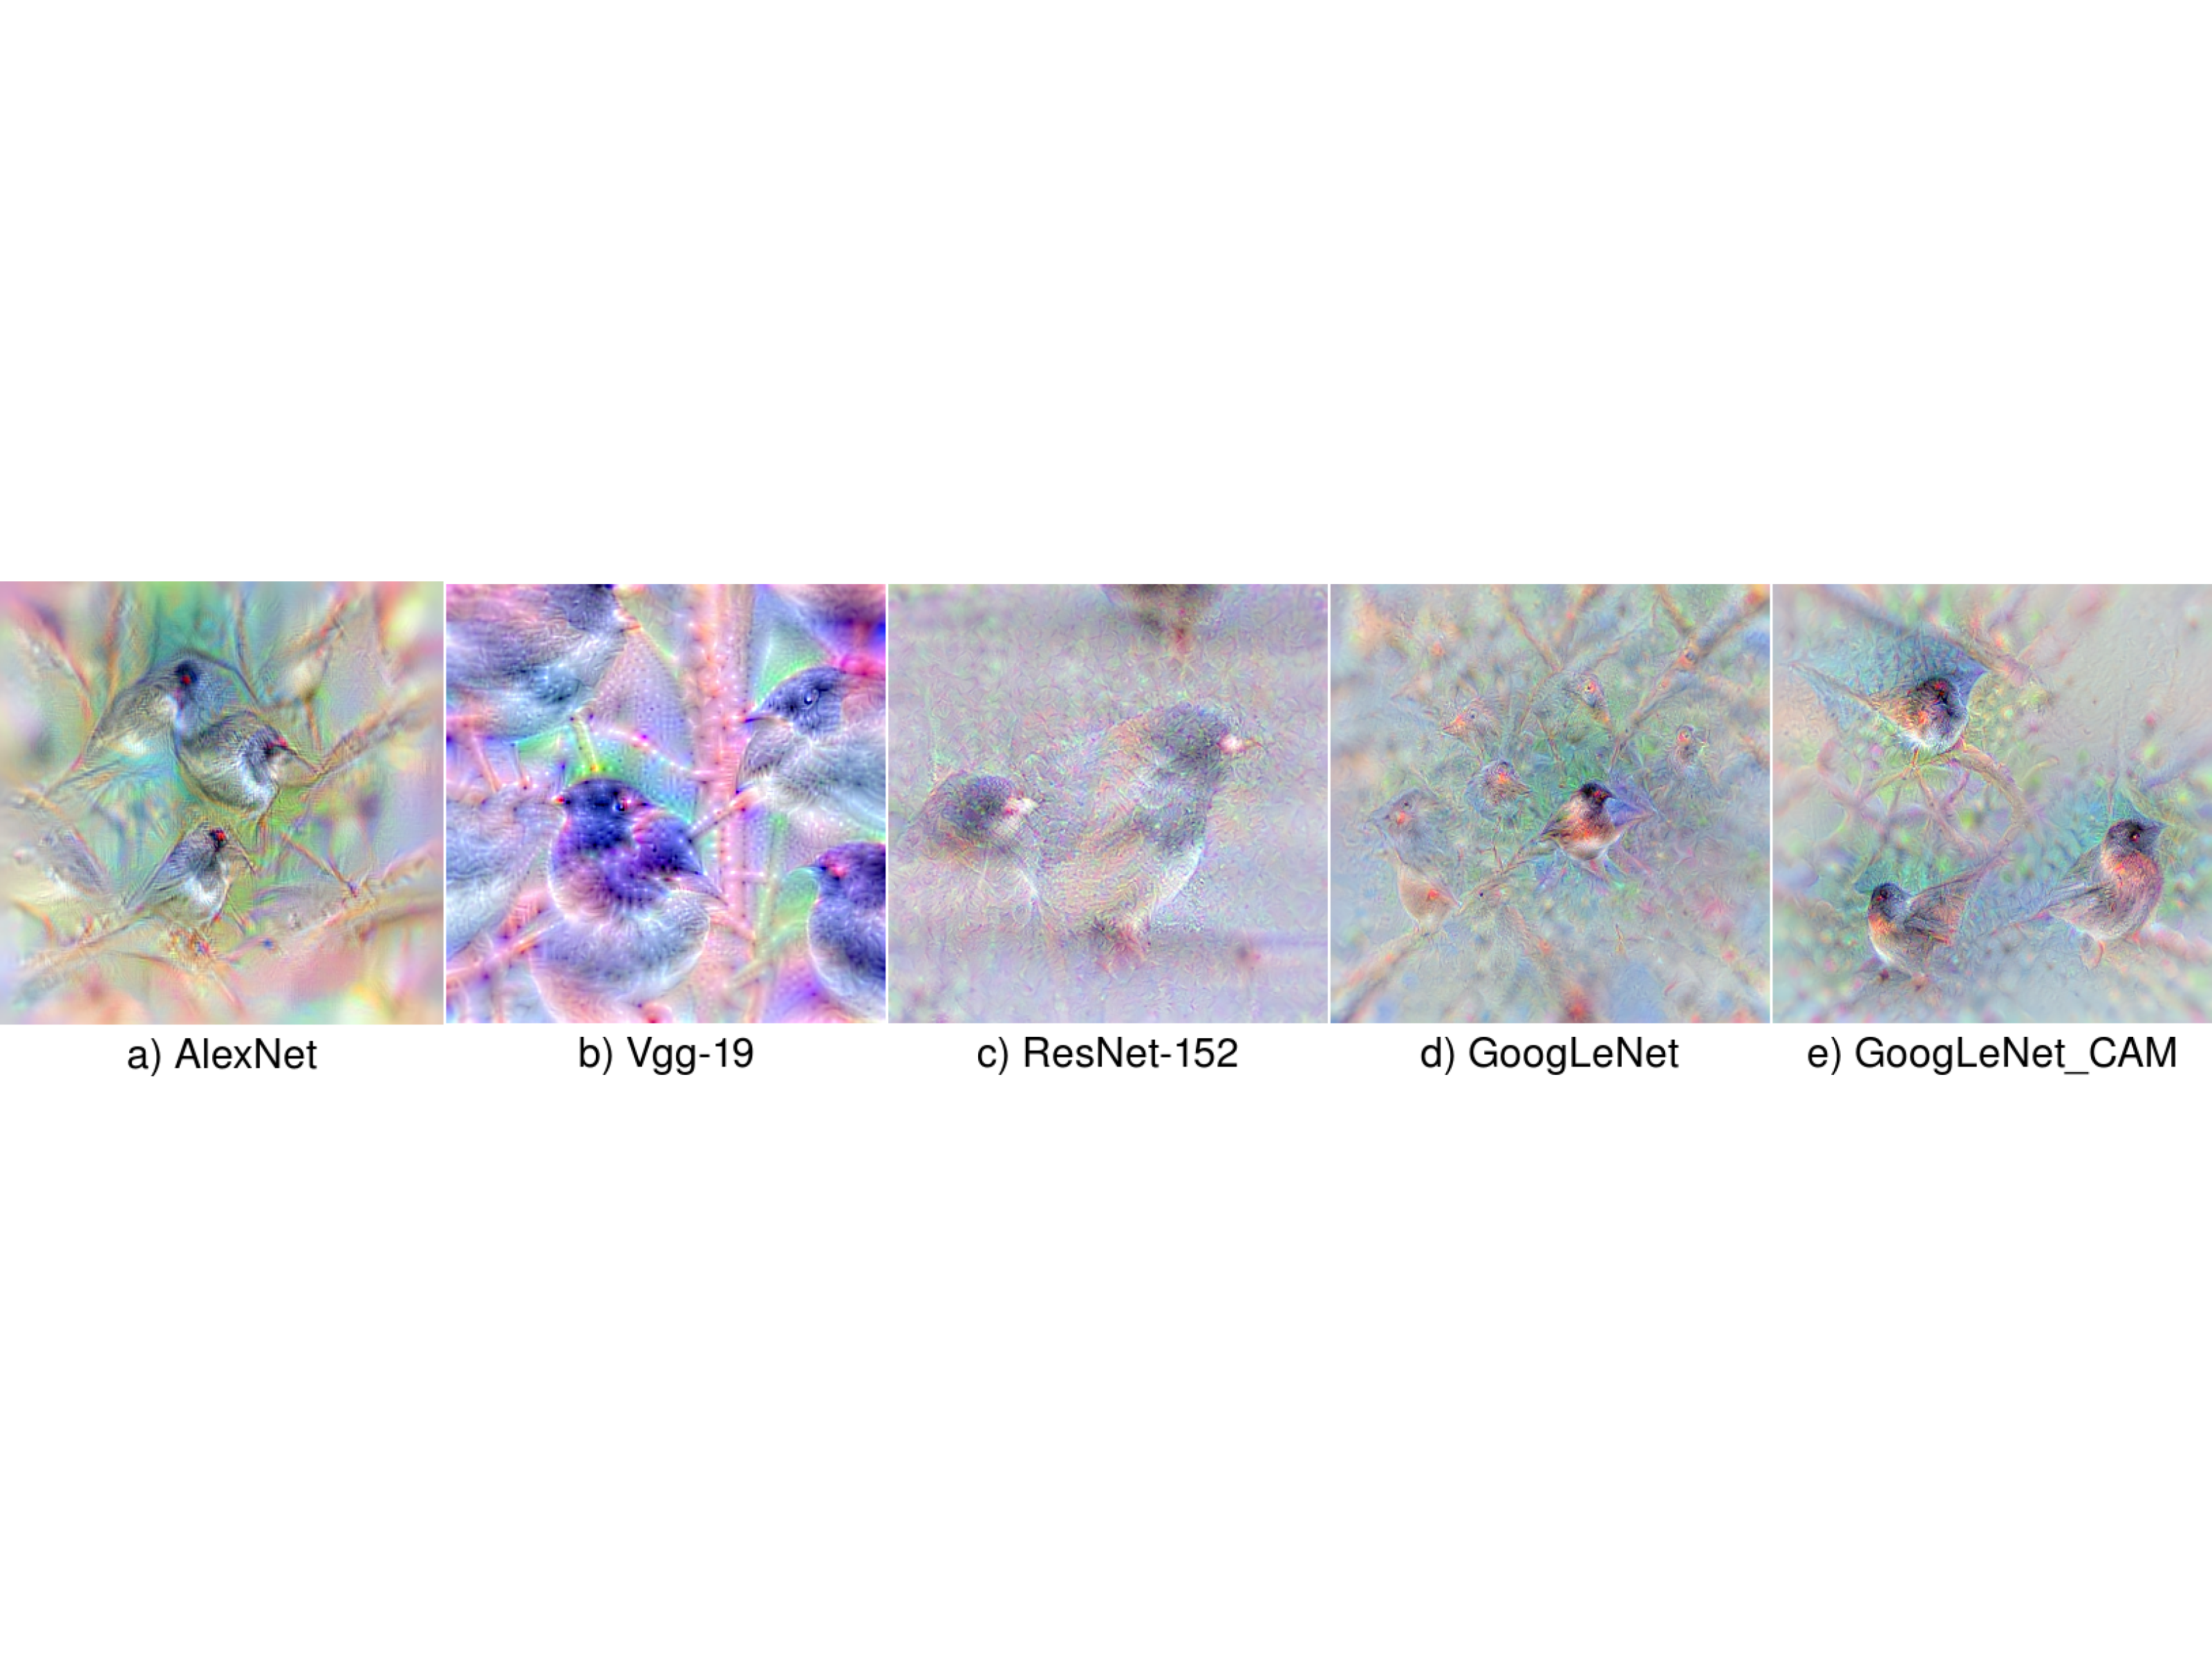
\includegraphics[trim = 0mm 60mm 00mm 60mm, clip, width=0.85\textwidth,,height=0.4\textheight]{ch04_02}
%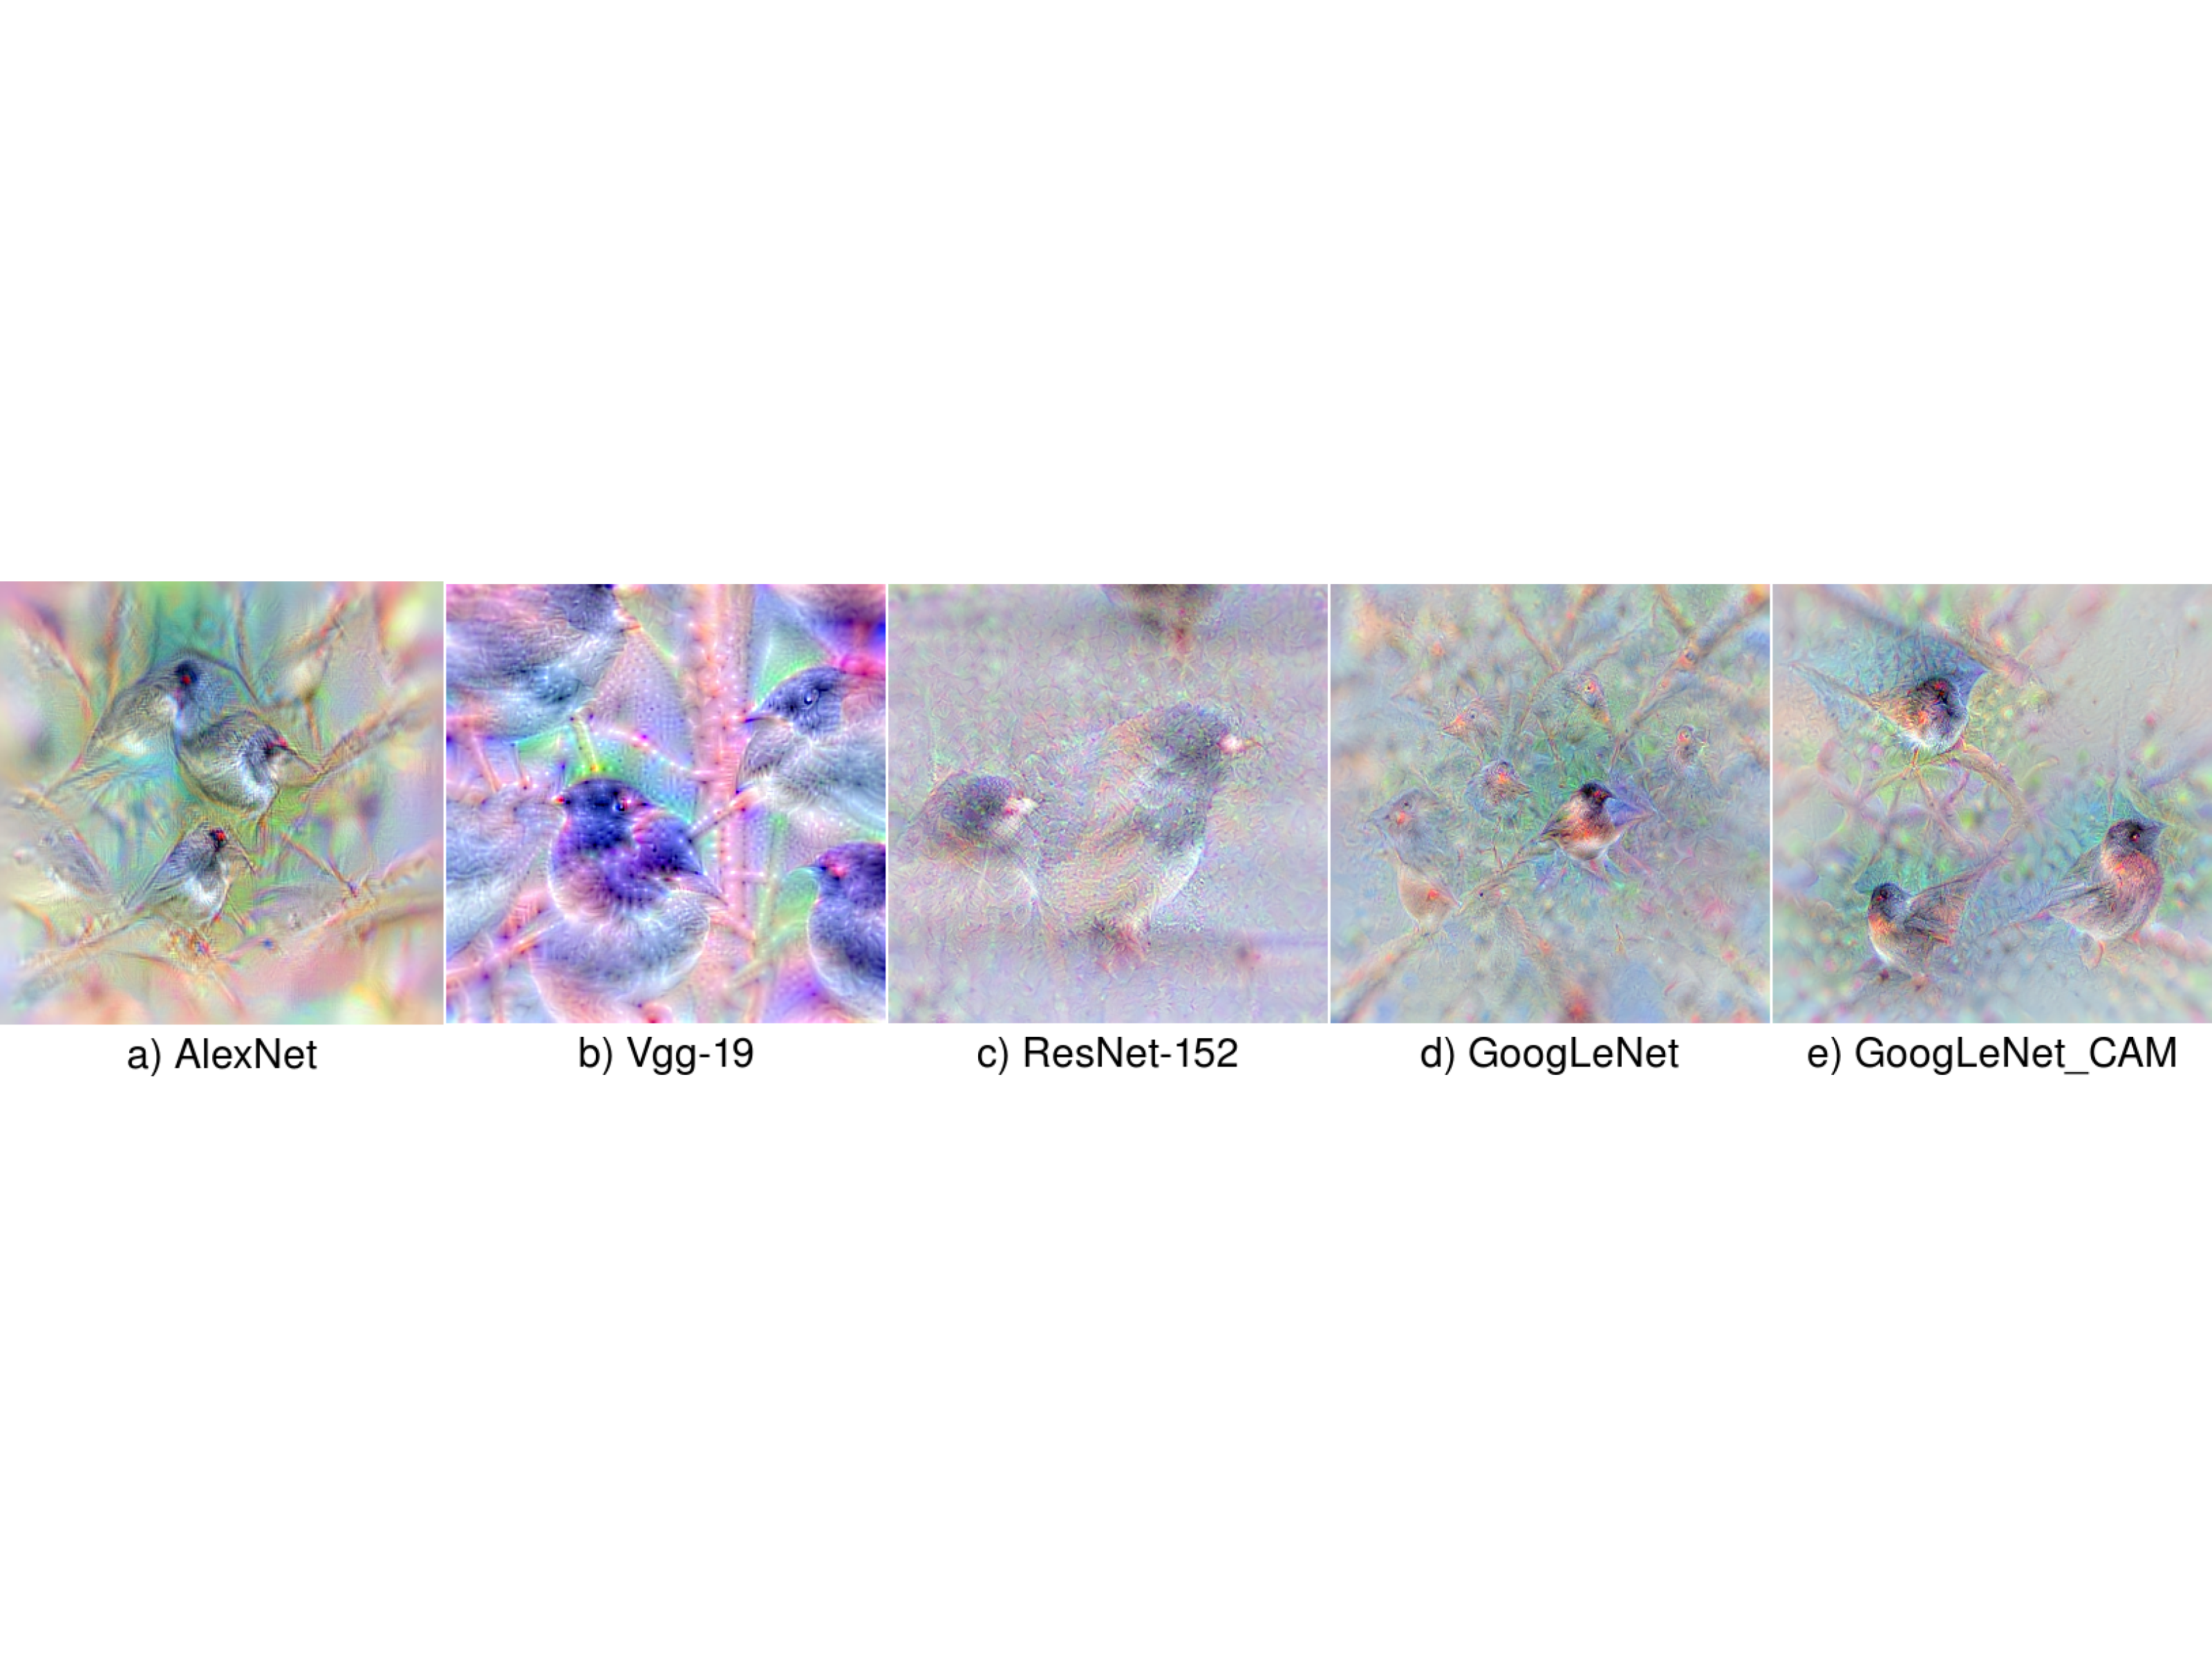
\includegraphics[width=0.85\textwidth]{ch04_02}
\caption{不同模型类别可视化实验结果}
\label{fig:ch04_02}
\end{figure}

4.2 不同正则化方法的类别可视化
为验证不同正则化方法对理解深度模型的特征表达的影响,采取前文所述的不同正则化方法,可视化效果结果见图\ref{fig:ch04_03}所示,从上到下依次可视化类别为金甲虫,海星,蝎子,酒壶,卷笔刀。
 
\begin{figure}[!htbp]
\centering
%trim option's parameter order: left bottom right top
%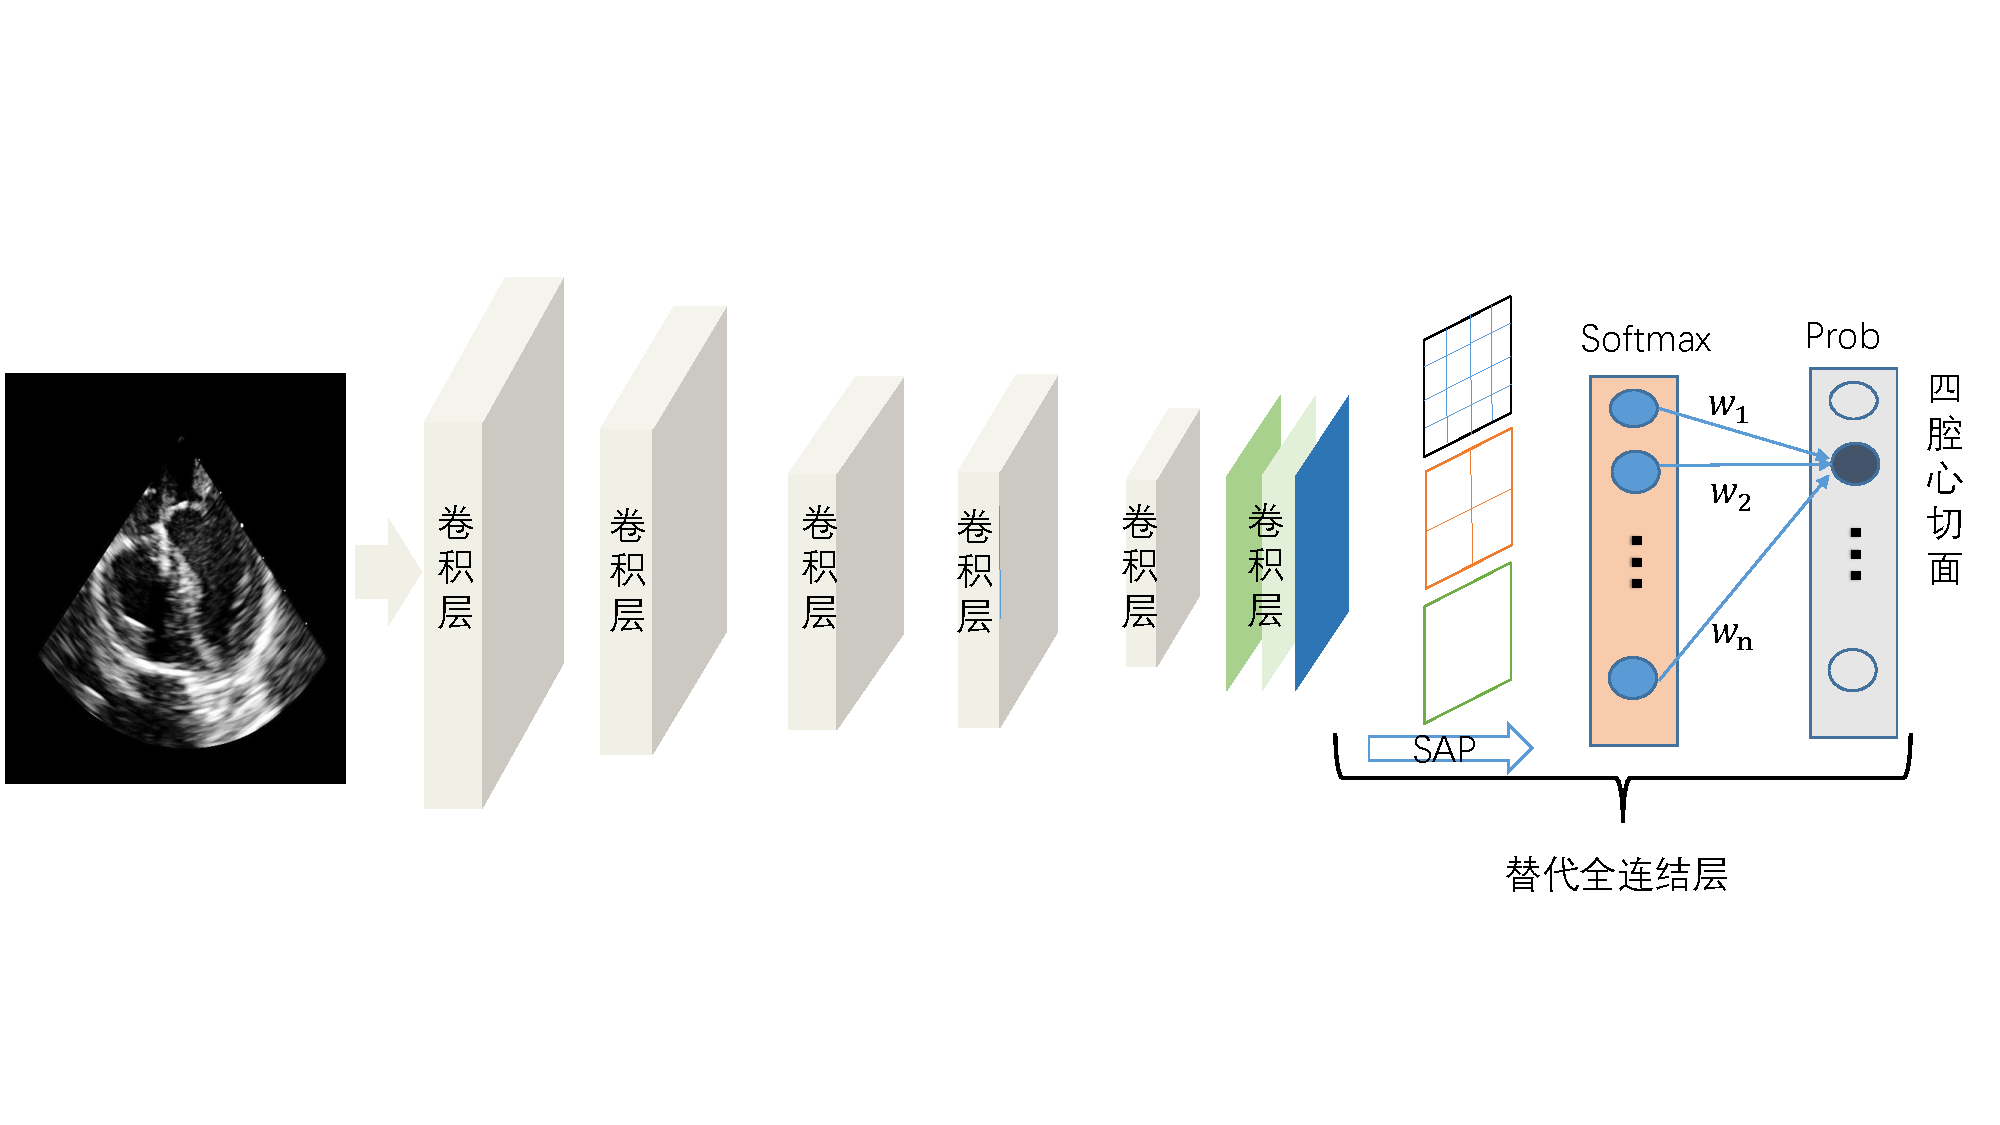
\includegraphics[trim = 30mm 0mm 30mm 0mm, clip, width=0.45\textwidth]{ch03_02}
\includegraphics[width=0.85\textwidth,,height=0.4\textheight]{ch04_03}
\caption{不同正则化方法的可视化效果}
\label{fig:ch04_03}
\end{figure}

图\ref{fig:ch04_03}中(a)列仅施加默认设置和不加梯度归一化的结果,由于输入的随机性,并不能保证每次都生成有意义的可视化结果,但引入本文提出的梯度归一化后,能大概率生成可视化结果见图\ref{fig:ch04_03}(b)列所示,图\ref{fig:ch04_03}(c)列表示只采用p范数正则化,跟文献\citep{•}2]一致取2,使得图像更平滑,但仍与真实图像相差较大。通过前文理论分析和实验验证,全变分跟高斯模糊作用类似,本文采用根据迭代轮数动态调整高斯模糊核大小,具体是在刚开始采用较大值希望生成物体大概轮廓,随迭代逐渐调小模糊核使得更多细节生成,具体见图\ref{fig:ch04_03}(d)。但是这个参数无法自适应设置为最优,对图像高低频分量无法调整控制,而本文提出的利用金字塔分解正则化方法能从粗到细调整,产生较优结果见图\ref{fig:ch04_03}(e)列所示。
4.3 金字塔分解可视化实验结果
为验证提出金字塔分解正则化方法,对中间层卷积核的可视化,采用前文提出式(8),指定深度CNN模型中不同卷积层中不同通道,利用前文提出的带动量的梯度更新策略,可视化结果见图4,其中从上到下依次为GoogleNet模型低中高层不同通道的可视化结果,与文献[7]一致,低层多尺度分辨率生成的纹理见图4首行所示,中层是一些物体部件,见图4中间行所示蜜蜂的局部结构,而高层是更完整的抽象概念见图4下层中完整的花瓣。对比图4(b)、(c)列,可验证拉普拉斯金字塔主动分解提升图像部分低频成分,而高斯金字塔分解生成的图像中高频细节更突出。
\begin{figure}[!htbp]
\centering
%trim option's parameter order: left bottom right top
%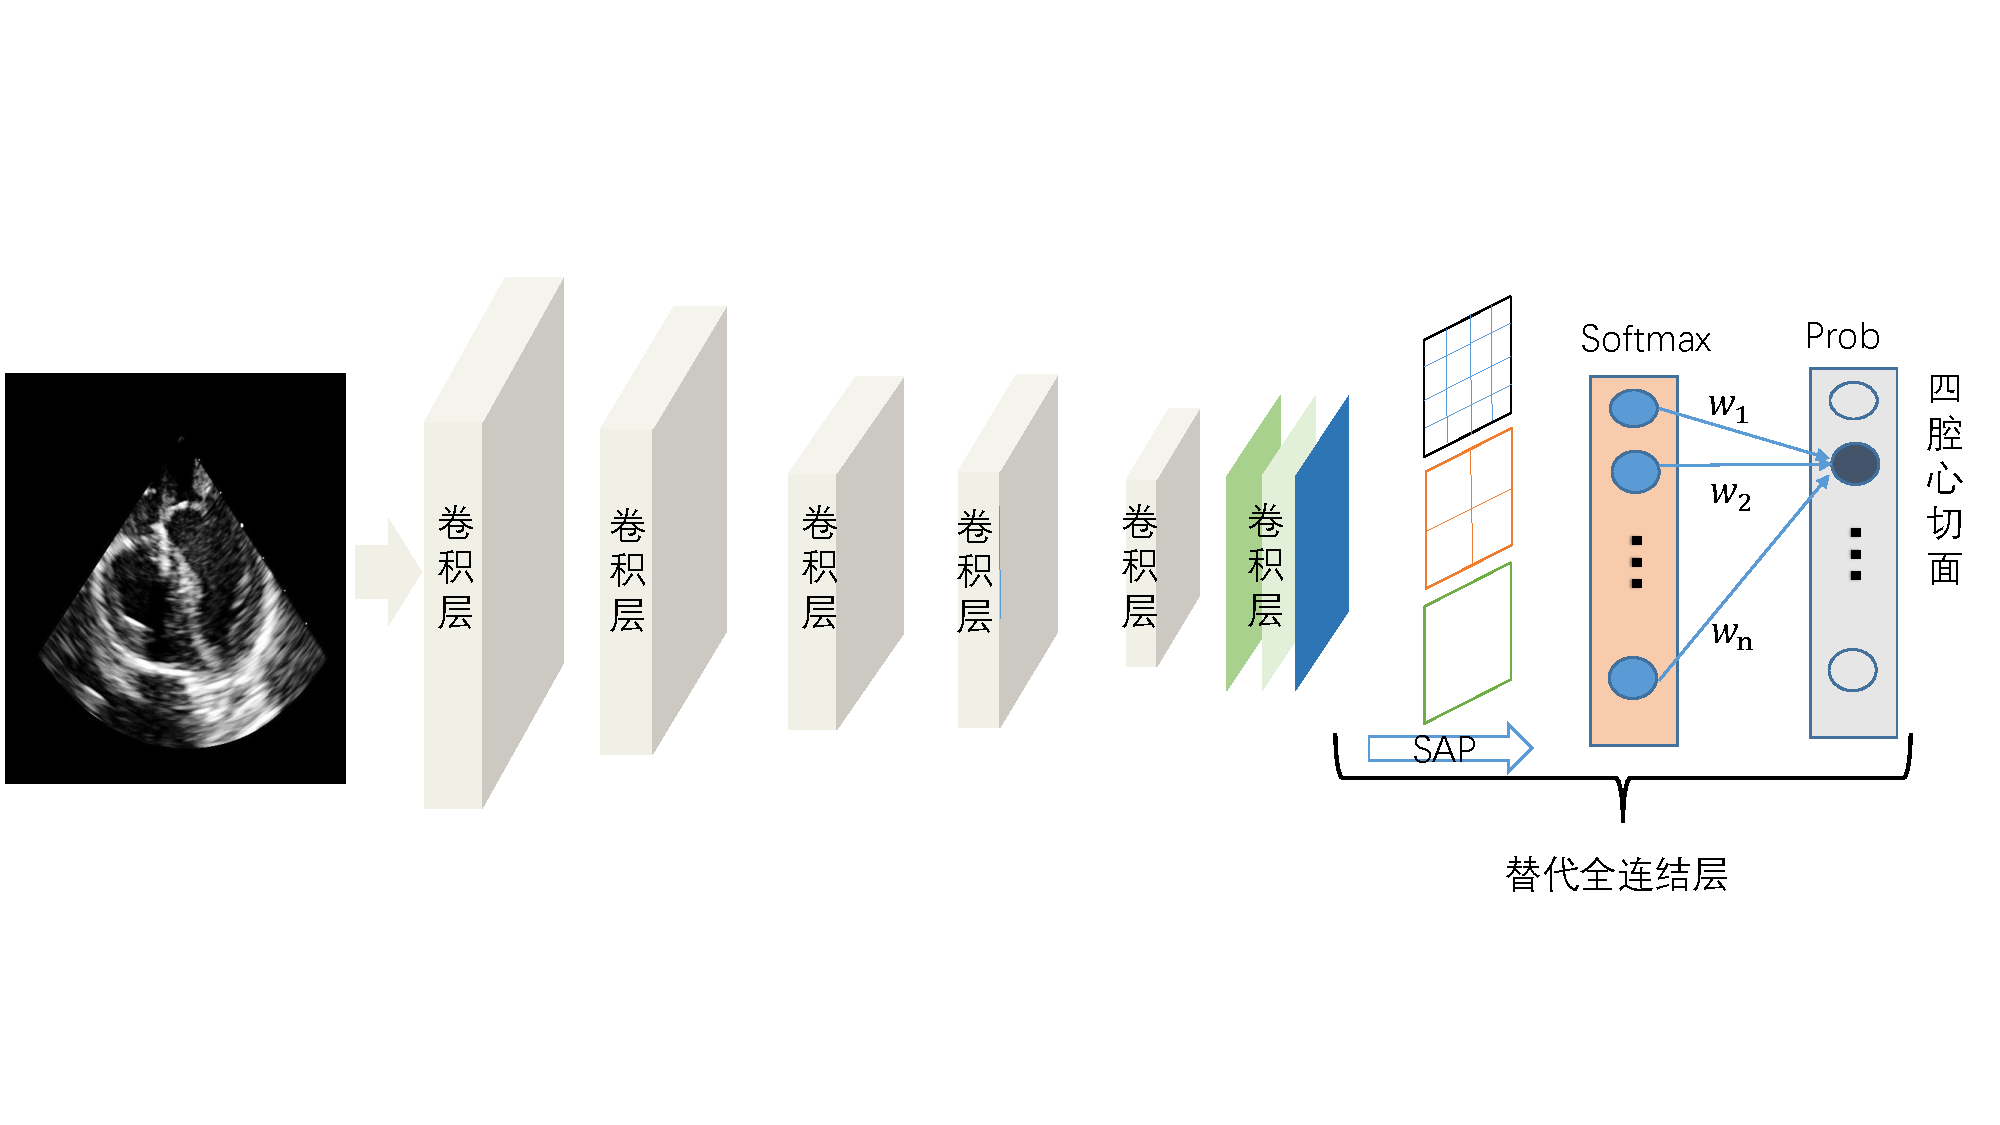
\includegraphics[trim = 30mm 0mm 30mm 0mm, clip, width=0.45\textwidth]{ch03_02}
\includegraphics[width=0.85\textwidth,,height=0.4\textheight]{ch04_04}
\caption{金字塔分解正则化可视化效果}
\label{fig:ch04_04}
\end{figure} 

4.4 引入类别显著性的可视化
通过观察之前可视化结果可知,生成的图像中除了该类别外仍有许多额外的上下文信息(见图2中鸟类别的树枝),这些信息与模型的分类能力相关联,可通过引入类别激活图可改善可视化效果。迭代更新过程中依据采用式(11),使用类别激活图作为加权因子限制迭代更新区域。
\begin{figure}[!htbp]
\centering
%trim option's parameter order: left bottom right top
%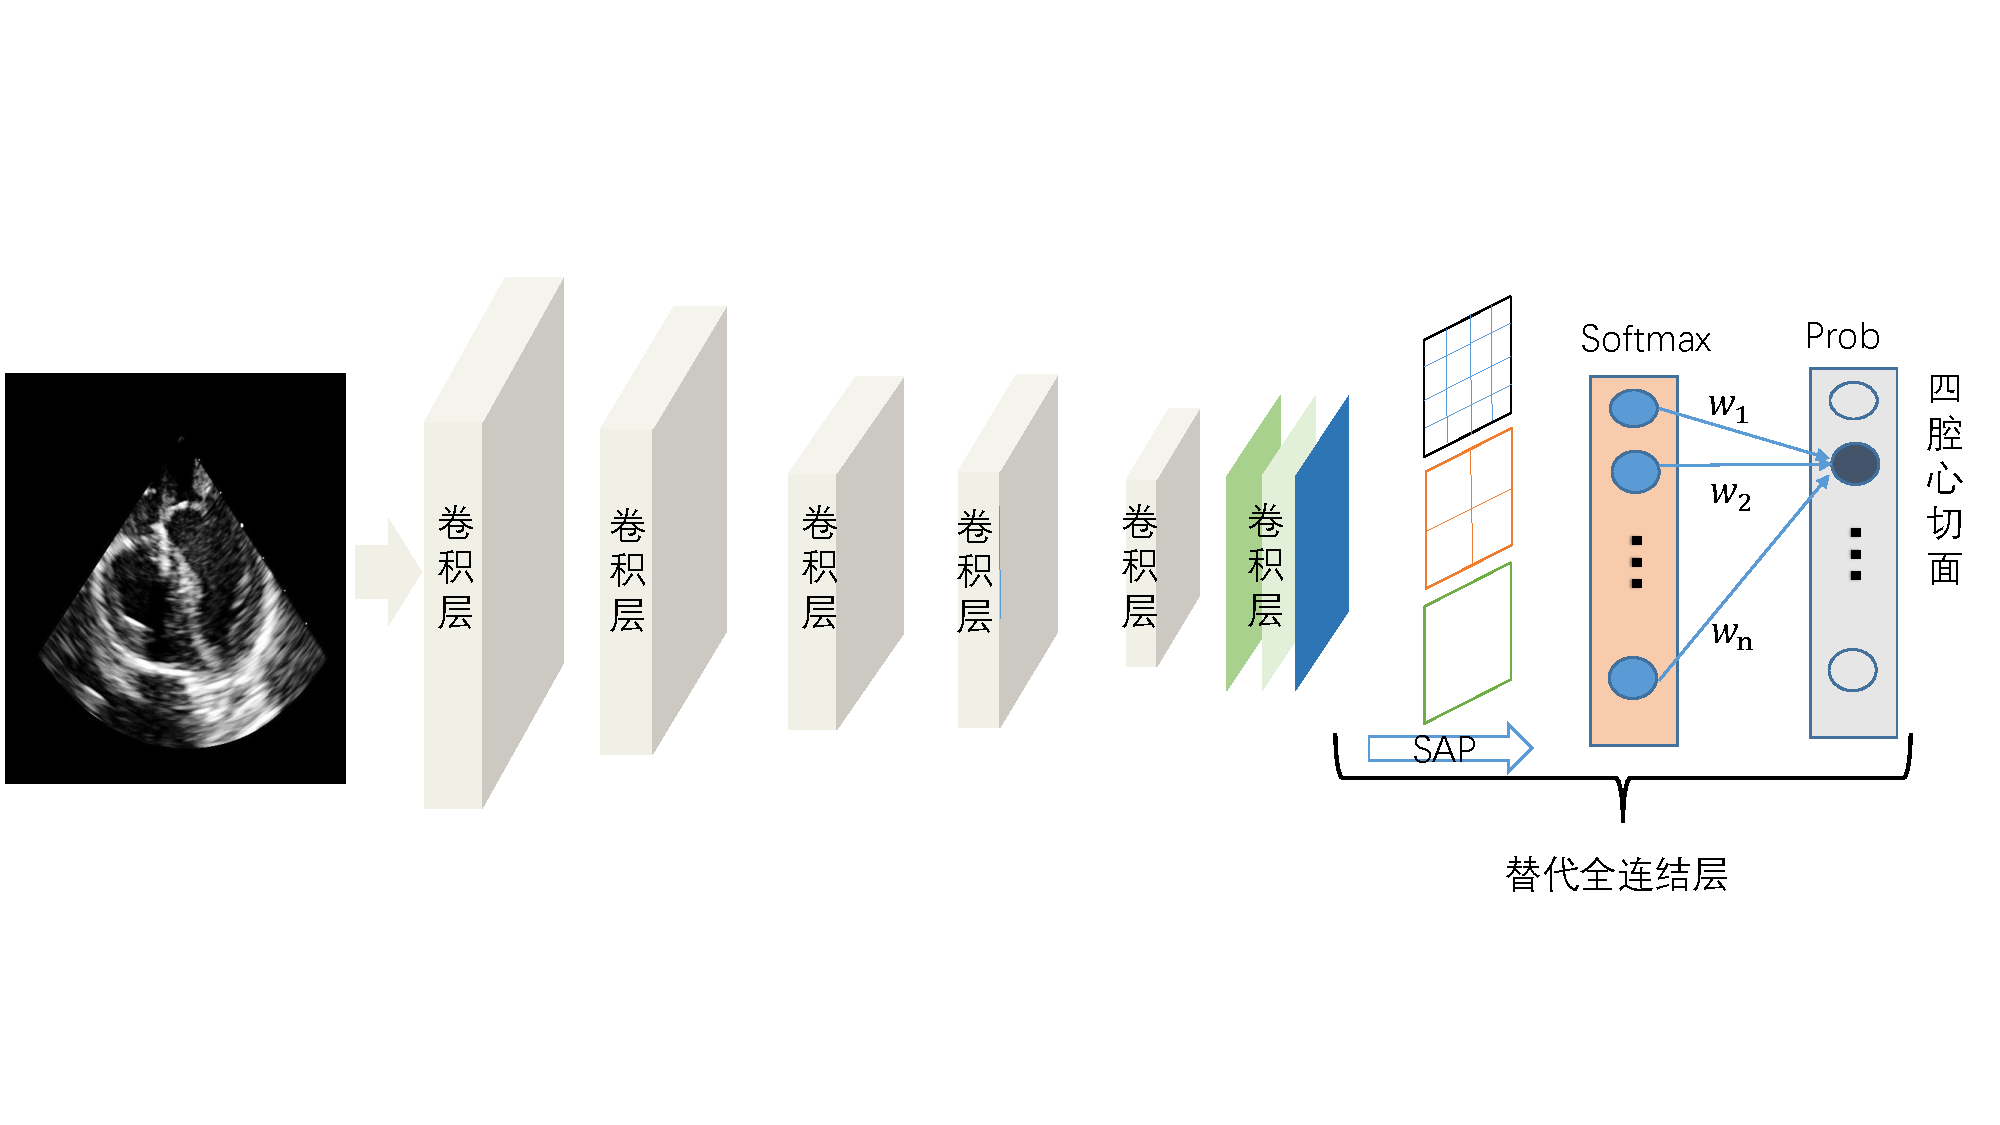
\includegraphics[trim = 30mm 0mm 30mm 0mm, clip, width=0.45\textwidth]{ch03_02}
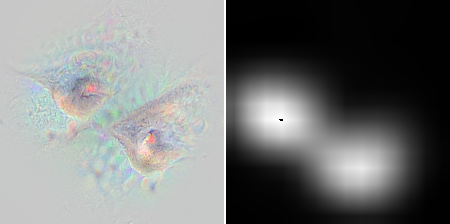
\includegraphics[width=0.85\textwidth,,height=0.2\textheight]{ch04_05}
\caption{引入类别激活图的可视化}
\label{fig:ch04_05}
\end{figure}  

实验结果见图5(a)所示,具体实验设置和图2采用的参数一致,使用提出的金字塔分解正则化技术,图5(b)为图5(a)相应的类别激活图,图5(a)结果表明与类别无关的上下文信息得到压制,但仍存在两个类别中心。

\section{本章小结}
本文针对理解深度CNN特征空间存在的问题,提出一种用于改善深度CNN分类模型的可视化方法。其中通过改善激活最大化可视化技术来产生更具有全局结构的细节、上下文信息和更自然的颜色分布的高质量图像。该方法首先对反向传播的梯度进行归一化操作,在常用正则化技术的基础上,提出使用空间金字塔分解图像不同频谱信息;为限制可视化区域,提出利用类别显著激活图技术,可以减少优化产生重复对象碎片的倾向,而倾向于产生单个中心对象以改进可视化效果。激活最大化可显示CNN在分类时关注什么。这种改进的深度可视化技术将增加我们对深层神经网络的理解,进一步提高创造更强大的深度学习算法的能力。该方法适用于基于梯度更新的可视化领域,是对网络模型整体的理解,具体各层特征怎么耦合成语义信息仍需进一步探索,深度CNN模型如何重建一个完整的类别概念,仍是一个开放性问题。

\chapter{医学计算机辅助检测方法}
\label{chap:Detection}

 提出了一种基于深度卷积神经网络自动识别超声心动图标准切面的方法,并可视化分析了深度模型的有效性。该算法针对网络全连接层占有模型大部分参数的缺点,引入空间金字塔均值池化替代全连接层,获得更多的空间结构信息,并大大减少模型参数、降低过拟合风险,通过类别显著性区域将类似注意力机制引入模型可视化过程。通过超声心动图标准切面的识别问题案例,试着对深度卷积神经网络模型的鲁棒性和有效性进行了解释。在超声心动图上的可视化分析实验表明,通过改进方法的深度模型的识别决策依据,同医师辨别分类超声心动图标准切面的依据一致,表明了方法的有效性和实用性。

\section{引言}

计算机辅助检测(Computer-Aided Detections, CADs)是医学影像诊断过程中的一项重要任务,是进行相关结构功能测量的前提条件。其中,二维图像的目标组织结构自动检测是CADs技术的核心基础。在临床实践中,医生需整合不同模态、不同位置方向且以不同比例显示的图像信息,目前的研究主要关注如何使检测过程快速自动化。由于医学影像自身的特殊性,比如缺乏大量高质量标注数据;大多数医学目标组织结构存在非刚性形变;图像背景前景的区分不明显等,导致组织结构自动定位比较困难。现有大多数CADs系统在临床实际应用中表现不佳的原因是:检测结果的敏感性和特异性都较低,诊断效能低\citep{Cheng2016a}。


不同模态的医学图像中,如超声、计算机断层扫描(Computed Tomography, CT)和核磁共振(Magnetic Resonance Imaging, MRI)等,都存在目标身体器官自动定位的问题。以左心室(Left Ventricle, LV)检测为例,大多数LV定位方法主要依据位置,时间和形状的假设。基于位置的方法仅假设心室在图像的中心,该方法并不对不同病人心室位置的差异性以及图像的尺寸变化进行考虑,效果较差;基于时间的方法,假设左心室是图像中唯一的运动对象,然而这种方法敏感性高,除心室的运动伪影之外,还存在其它运动的器官,如Schollhuber\citep{Schollhuber2008}针对MRI短轴使用时空信息并消除运动伪影,由分层模式匹配算法定位包含LV的感兴趣区域,其通过使用互信息图像配准使运动伪影最小化,随后估计特征强度—时间曲线进行像素分类和边界的提取,得到最终分割结果;基于形状的方法将LV视为圆(短轴)、椭圆(长轴),然而该方法通常针对异常形状的LV容错性差,如Lu等\citep{Lu2009}使用大津阈值度量圆形程度,然后进行霍夫变换定位LV位置。也可搜索每个切片的质心,并用三维最小二乘拟合去除异常值,得到分割结果\citep{Petitjean2011}。


不依据具体的强先验假设,机器学习算法可通过区分前景目标对象和背景来解决目标结构自动检测的问题。如Kellman等\citep{Lu2011}提出了一种使用概率集成提升树来估计LV姿态和用空间间隔学习LV短轴边界的方法。Zhou等\citep{Zhou2005}在超声心动图中通过规一化集成提升回归学习非线性映射以定位LV,其团队后来提出针对多个器官的特异性置信最大化分类器,整合更高的自由度以改善回归定位任务的精度。Liu等\citep{She2007}通过利用基于子模块函数优化理论的多标记搜索策略来进行标记点的检测。Zheng等\citep{Zheng2014}在实现器官定位的同时,通过组合优化置信度来估计目标器官的位置、缩放及朝向等参数值。前述机器学习算法都基于弱先验知识,启发式设计相关特征,结合滑动窗口策略,选择分类器进行分类判断窗口中内容以估计相应位置。


近来通用物体检测领域取得巨大进展,主要得益于深度学习能利用大量标注数据,从原始像素出发,逐层分级学习中高层抽象语义特征\citep{Sharif2014}。区域卷积神经网络\citep{Girshick2014b}在大规模自然图像数据集(如ImageNet\citep{Russakovsky})上,识别性能远超传统方法\citep{Girshick2014b,Krizhevsky2012}。当前实践中由于深度学习需要大量的训练数据,所以仅在少数医学任务中取得有限的成功应用。深度学习方法用在定位检测问题时可分为两个阶段\citep{Girshick2015b}:候选框位置选取和窗口内容类别分类。如利用深度卷积网络进行显微镜图像中细胞检测\citep{Akram2016}、结合深度全卷积网络的MRI心室检测与分割\citep{Emad2015,Tran2016a}和超声图像解剖结构的检测\citep{Chen2016i}。这些方法大都关注特定目标结构的检测分割,而本文专门针对目前CADs普遍存在的检测定位问题,基于改进的生成候选框的快速区域深度卷积神经网络(Faster RCNN)\citep{Ren2015a}方法,提出一种医学目标结构检测框架:1)在区域生成网络的基础上引入空间变换损失使得候选框生成网络能捕捉目标的空间变换参数;2)采用在线困难样例挖掘策略,加快训练收敛过程,提高检测小目标的准确度;3)并基于目标先验知识,针对左心室提出利用检测二尖瓣环、心内膜垫和心尖位置,高效估计左心室姿态参数。4)为验证该算法的鲁棒性和有效性,分别针对两个具体CADs应用进行实验分析。

\section{区域卷积神经网络概览}
 
\subsection{物体检测形式化定义}
若用$r$来表示图像中的矩形窗口区域,令$R$表示由对象检测系统提供的所有候选窗口的集合,将有效定位标记定义为$R$的子集,使得标记位置内内容“不重叠”,令$Y$来表示所有有效标记位置的集合。并合并常用的非最大值抑制(Non-maximum suppression, NMS)过程,给定图像$x$和窗口评分函数$f$,物体检测算法流程可定义为:
\begin{table}[htbp]
 \caption{\label{tab:Algorithm1}算法 1 物体检测}
 \begin{tabular}{l}
  \toprule
  Input: 图像x,窗口得分函数f  \\
  \midrule
  1:  $D$:= 所有候选框 $r \in 使得$f(x, r) > 0$ \\
  2:  按 $f$ 排序$D$使得 $D1 ≥ D2 ≥ D3 ≥ ...Dn$ \\
  3:  $y^∗$:$= {}$  \\
  4:  for $i = 1$ to $n$ do \\
  5:     若 $D_{i} 和 $y^∗$中任意候选框不重叠 \\
  6:          $y^∗$ := $y^∗  \bigcup {D_{i}}$ \\
  7:  end for\\
  \midrule
  8:  Return:  $y^∗$,物体的目标位置.
  \bottomrule
 \end{tabular}
\end{table} 
 
形式化定义物体检测过程见公式\ref{eq:ch05_01},式中参数定义请参考算法\ref{tab:Algorithm1}。
\begin{equation} \label{eq:ch05_01}
      y^∗=\mathop{\arg\min}_{y\in Y}\sum _{r\in Y} f(x,r)
\end{equation}                               	 
通常公式\ref{eq:ch05_01}可通过贪心搜索的方法来完成,算法将联合最小化在算法\ref{tab:Algorithm1}中产生假阳例的数量和最大化检测窗口评分函数,即寻找具有最大得分但同时不重叠的滑动窗口位置集合。
\subsection{区域卷积神经网络的演进}

2014年Gisrshick等\citep{Girshick2014b}提出区域卷积神经网络(Region-based Convolutional Neural Network, RCNN),对每一候选框窗口都进行一次前向传播,这将导致冗余计算,时间复杂度高,为解决这一问题,He和Ren等提出SPP-net\citep{He2015spp}和Fast RCNN\citep{Girshick2015b}加以改进,不再把每一候选窗口均送入网络,而是仅对图像特征提取一次,把原图中候选区域投影到卷积特征图上,然后对投影后的区域特征图进行空间感兴趣区域池化(ROI Pooling)得到固定长度的特征向量。其中Fast RCNN中的感兴趣区域池化是SPP-Net中多尺度空间金字塔池化的特例,仅用单一尺度的金字塔池化操作。RCNN及其改进的Fast RCNN都依赖于人为设计的候选框生成方法,如选择性搜索等。为减少生成候选框的计算时间,Faster RCNN提出区域生成网络(Region Proposal Networks,RPN),区域生成网络和检测网络共享提取特征的卷积层,仅提取几百个或者更少的高质量预选窗口,且召回率较高(导致更少的假阳例)。但现有的通用物体检测算法均是假设候选框为矩形,不能解决旋转朝向问题。

 
\section{候选区域生成网络及其改进}
 
本章将分别从候选区域生成网络模型的结构、仿射变换候选框区域的生成、空间变换损失函数的设计、模型训练方法等方面介绍本文所提出框架,并结合Faster RCNN模型提出端到端的目标检测方法。
\subsection{候选区域生成网络模型结构}

候选区域生成网络将一图像(任意大小)作为输入,输出目标候选框的集合和每个候选框内有无目标的概率估计,如图\ref{fig:ch05_01}右图所示,RPN在卷积层后接两个全卷积层完成候选区域生成功能,以实现增加滑动窗口操作。该模型使用全卷积网络[20]处理任意大小的图片输入,为了和目标检测网络\citep{Girshick2015b}共享计算,在特征提取的过程中同时计算目标检测所需的感兴趣区域的初始估计,在最后一个共享卷积层输出的特征映射图上滑动小网络,卷积特征映射图上n×n大小空间窗口作为该网络全连接的输入,本文n取3。每个滑动窗口映射到一个低维向量上(如图一左上中256-d),该向量输出给两个全连接层——候选框位置定位回归层和候选框类别分类层。原文中采用类别无关分类损失,即仅区分该候选框内是否包含物体(前/背景),本文将其扩展为类别相关的分类损失。
\begin{figure}[!htbp]
\centering
%trim option's parameter order: left bottom right top
%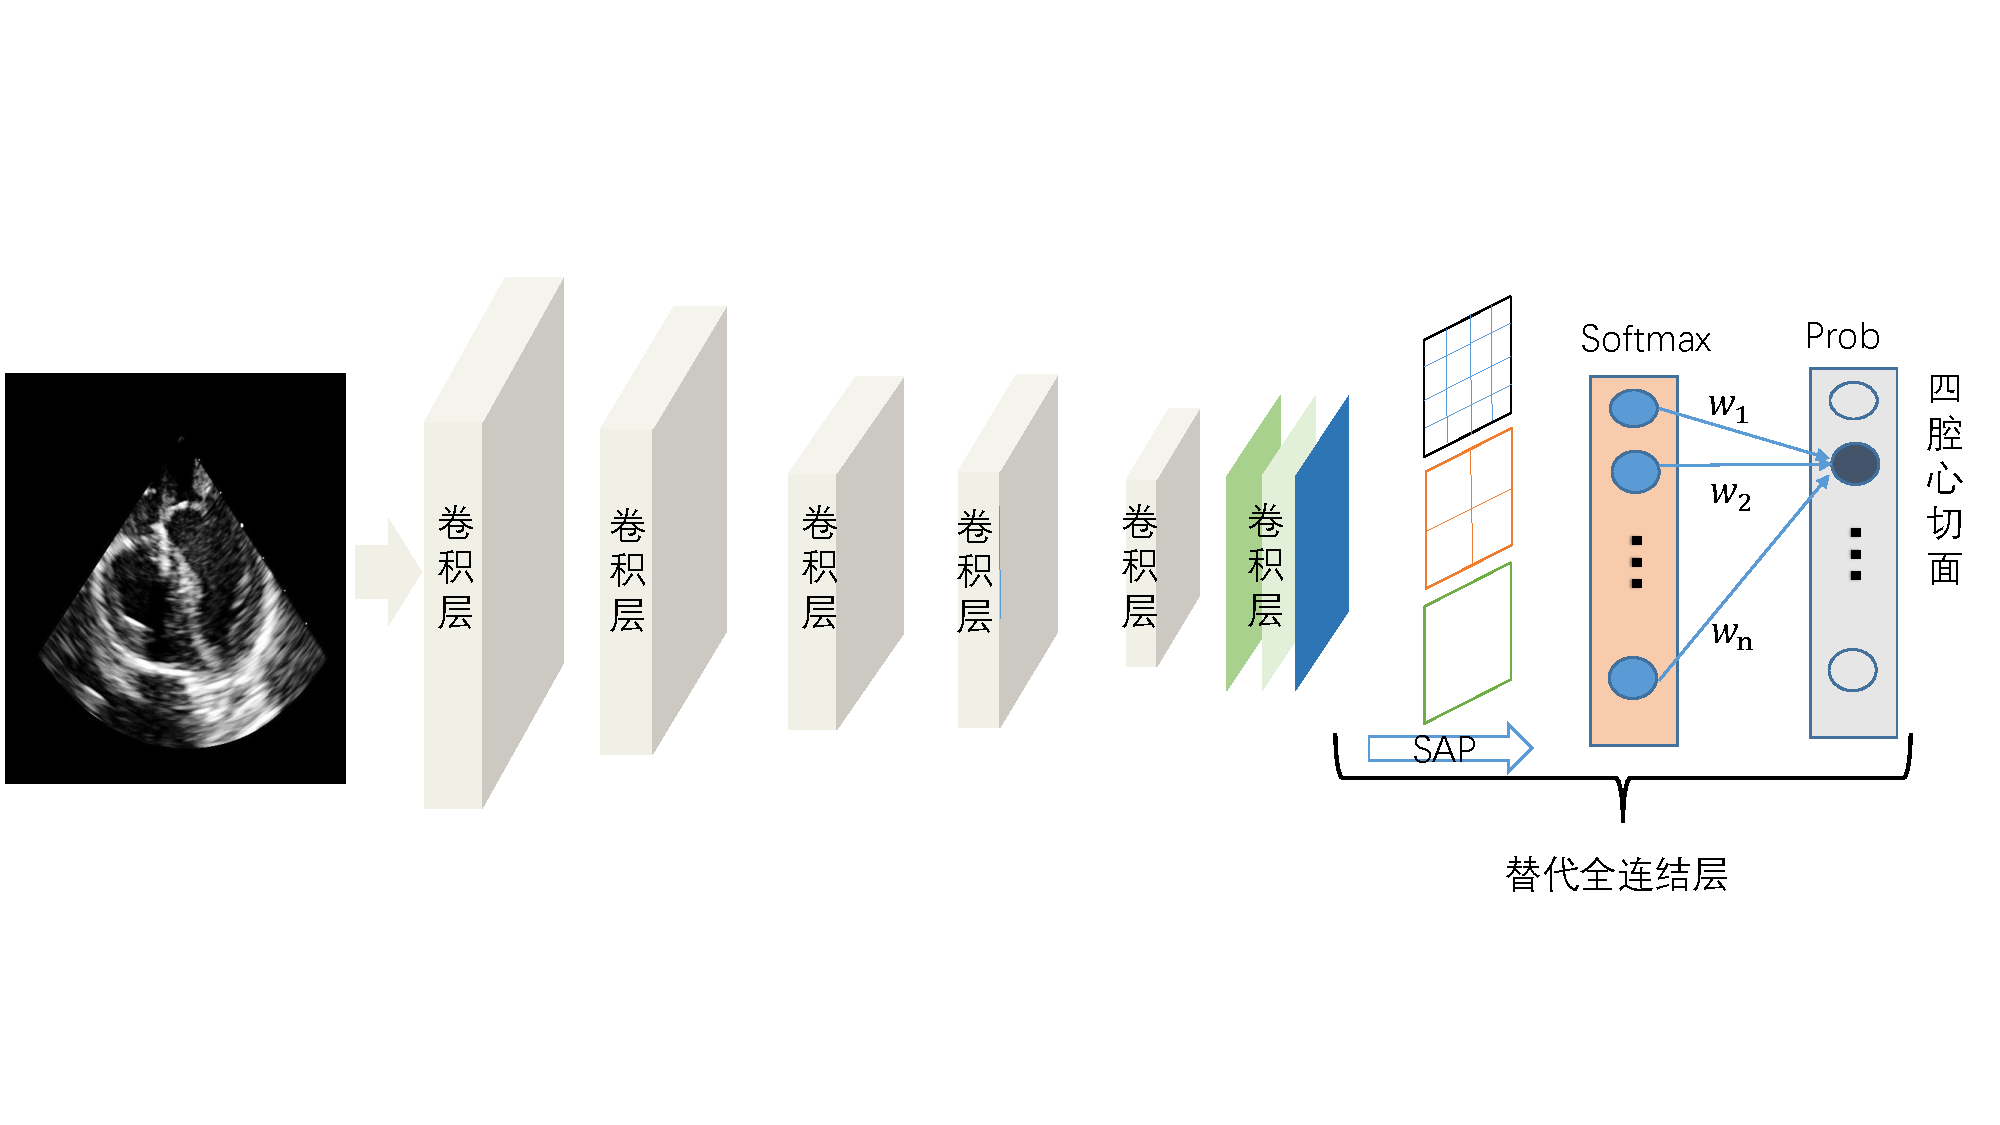
\includegraphics[trim = 30mm 0mm 30mm 0mm, clip, width=0.45\textwidth]{ch03_02}
\includegraphics[width=0.85\textwidth]{ch05_01}
\caption{左上:引入空间不变性的anchor机制  左下:空间变换网络  右:Faster R-CNN带仿射变换的检测模型框架}
\label{fig:ch05_01}
\end{figure}

为引入空间尺度不变性,采用多尺度和多纵横比的“参考”框(anchor)(图\ref{fig:ch05_01}左上所示)。该机制可看作是金字塔型参考框的回归,避免了枚举多尺度、多纵横比的图像或卷积核。在每一个滑动窗口的位置,同时预测k个参考区域,回归层有4k个输出,即k个box的坐标编码,多元逻辑回归分类层输出(c+1)×k个(物体类别数c加背景类的)概率估计。候选框由相应的k个anchor的参数化表示,每个anchor以当前滑动窗口中心为中心,并对应一种尺度和长宽比,我们使用3种尺度和3种长宽比,在每一个滑动位置就有k=9个anchor。对于大小为w×h的卷积特征映射,总共有$w×h×k$个anchor。
\begin{figure}[!htbp]
\centering
%trim option's parameter order: left bottom right top
%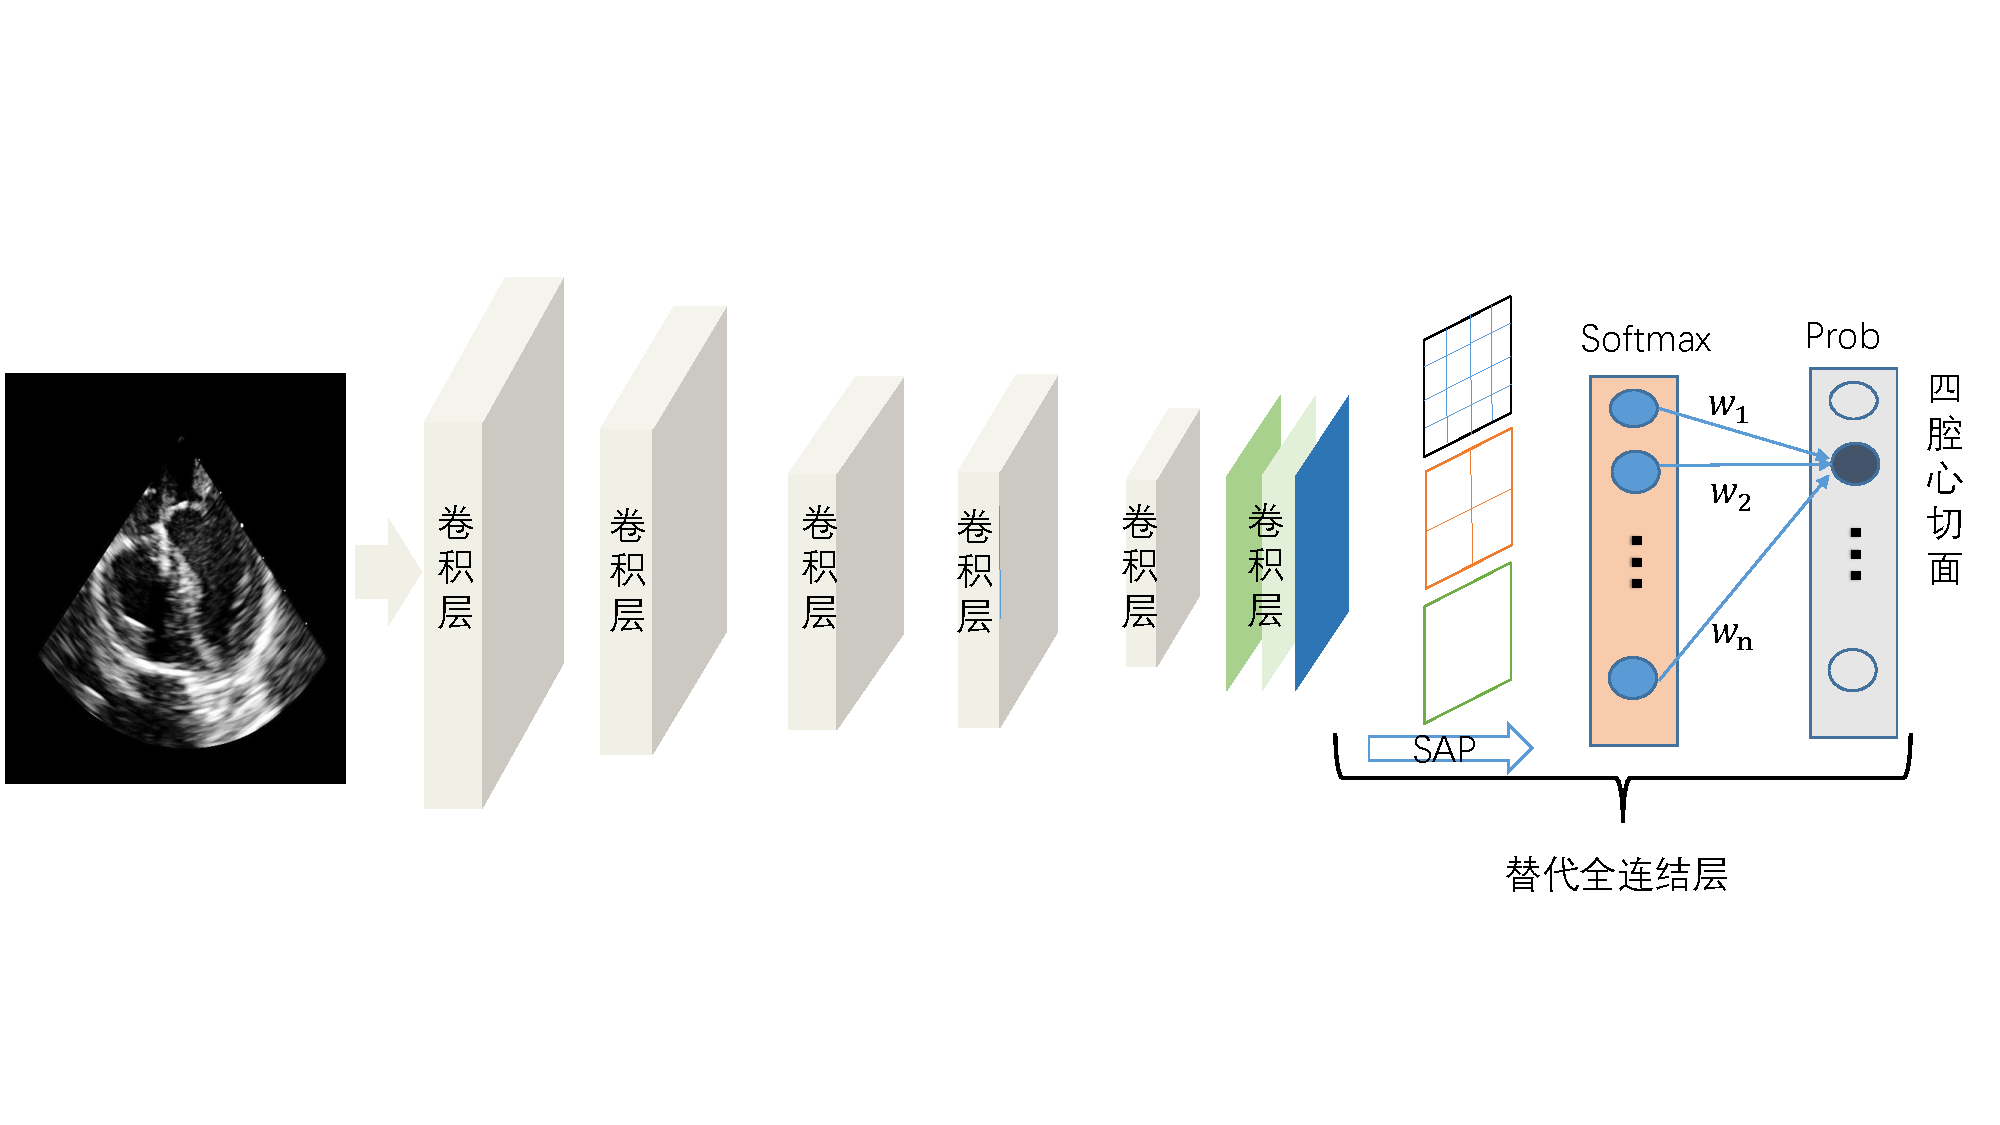
\includegraphics[trim = 30mm 0mm 30mm 0mm, clip, width=0.45\textwidth]{ch03_02}
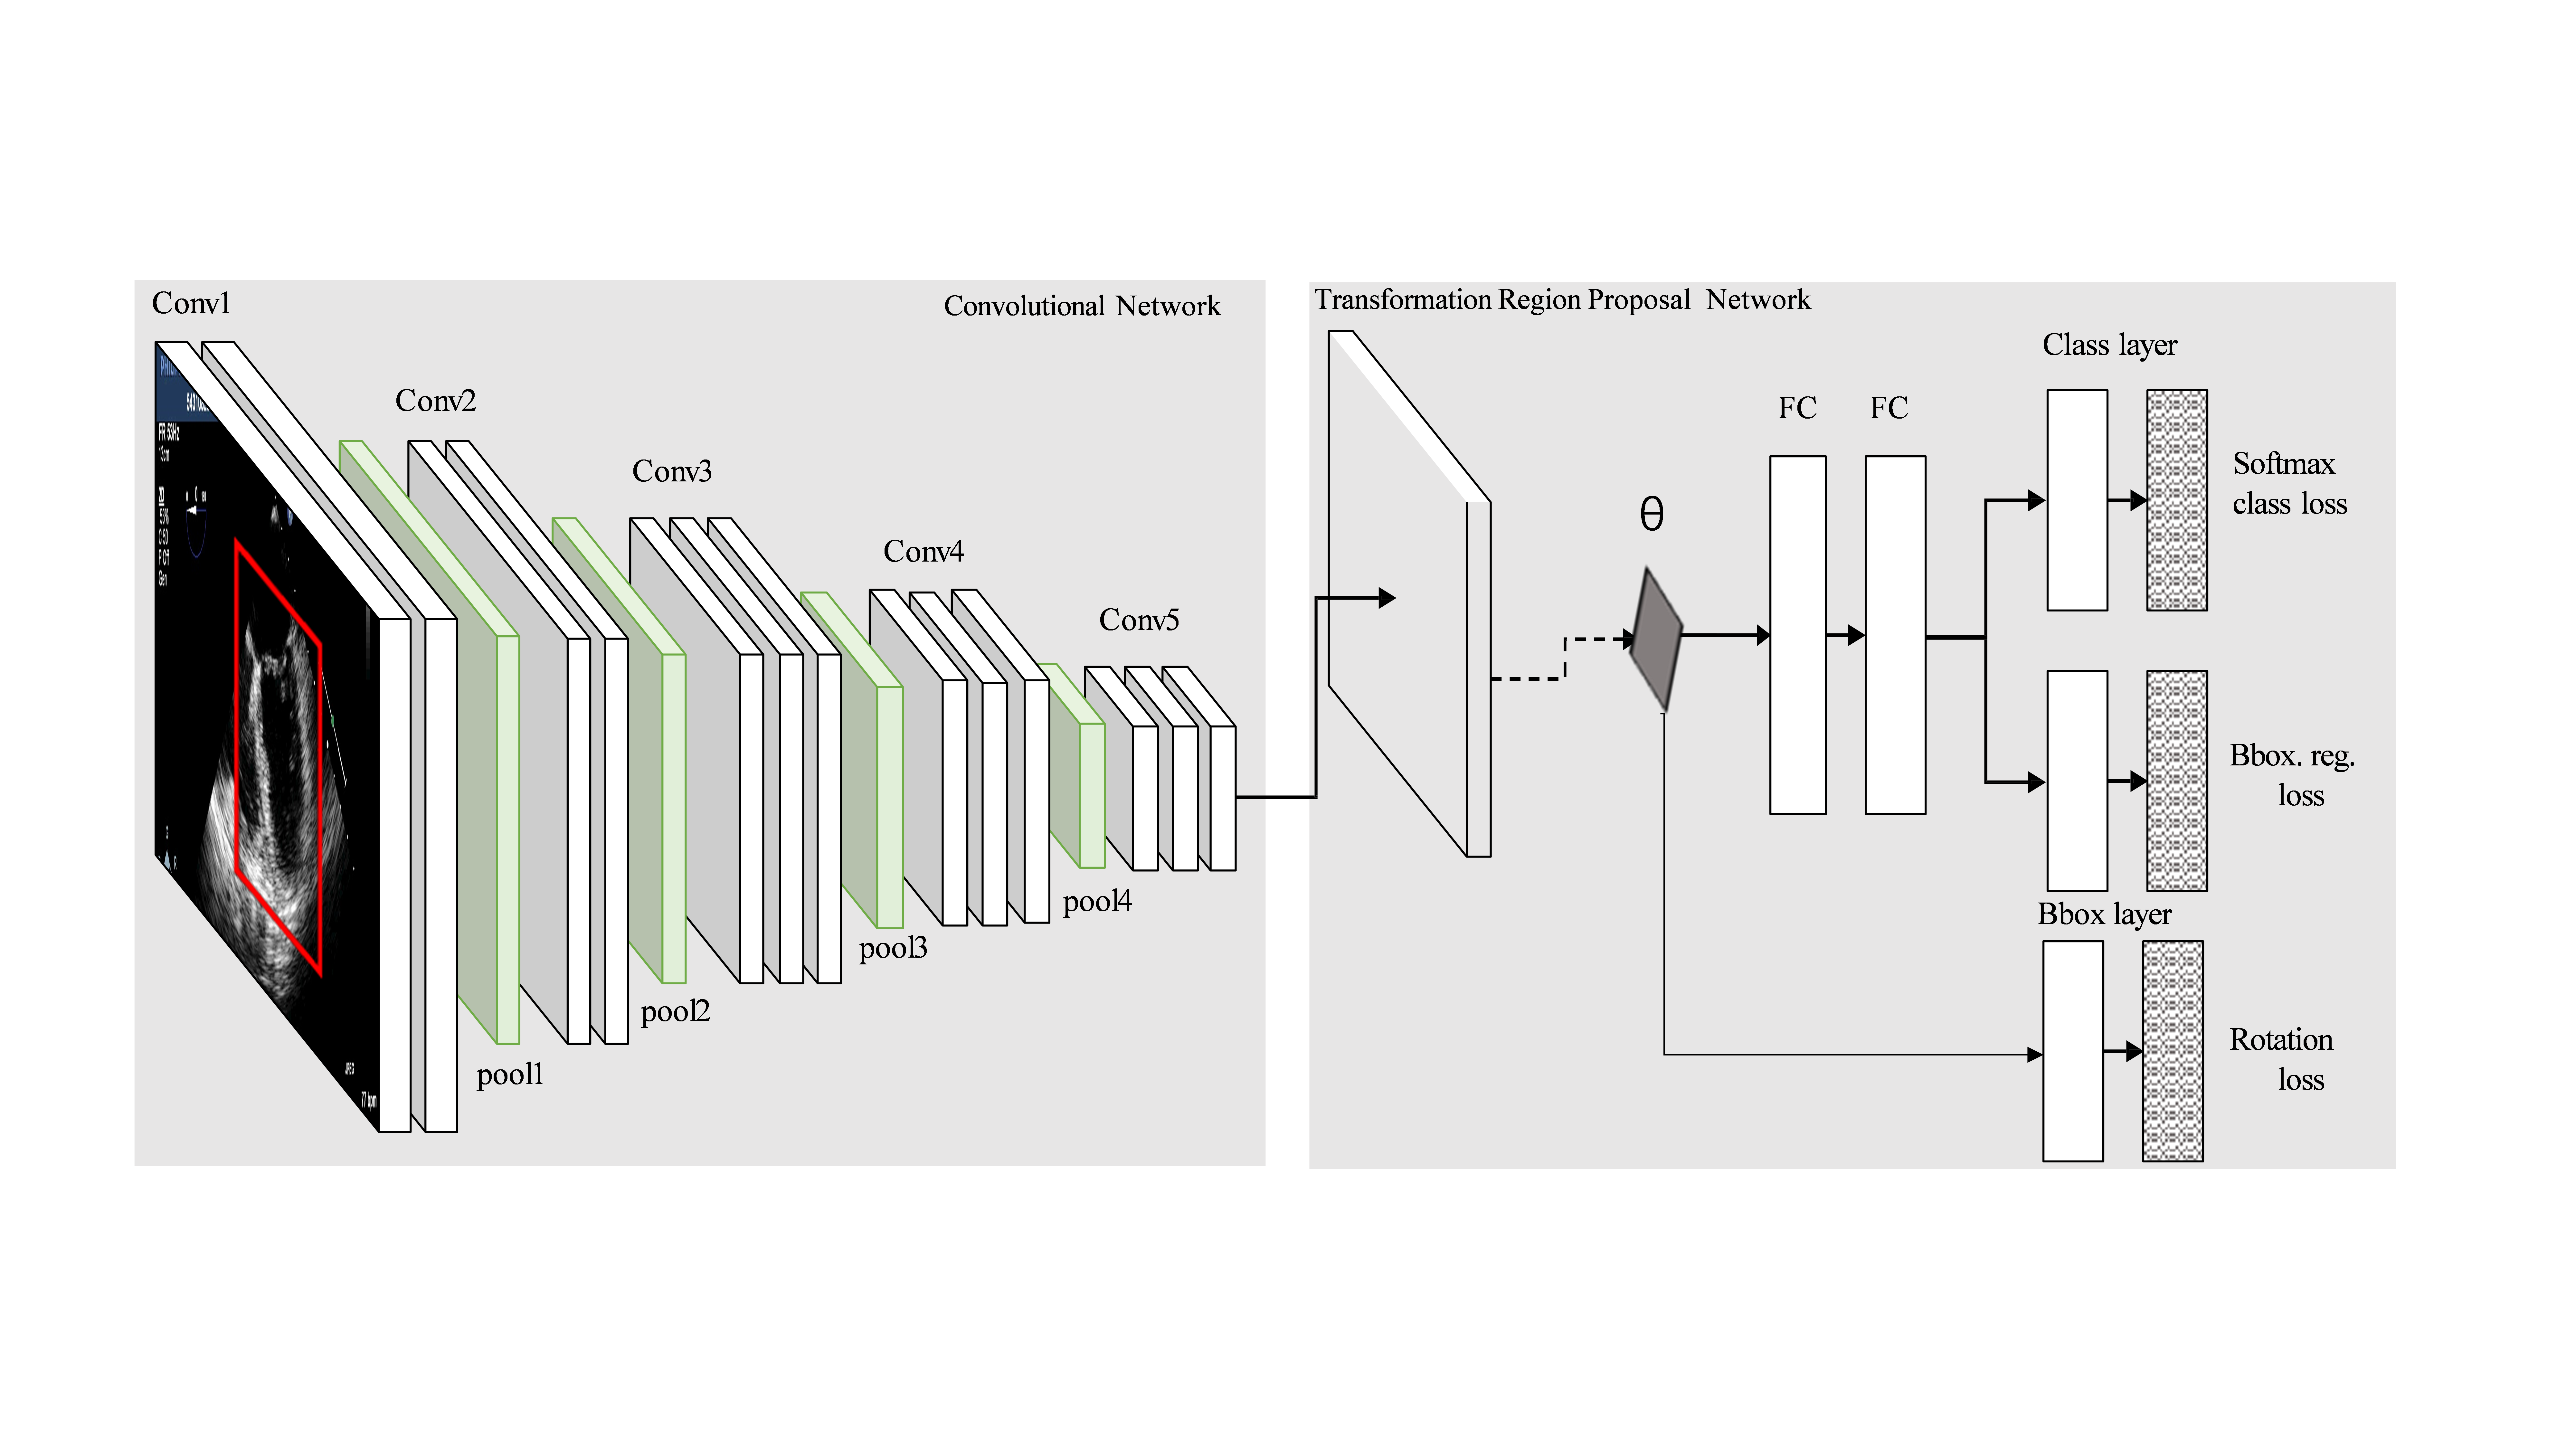
\includegraphics[width=0.85\textwidth]{ch05_02}
\caption{考虑物体朝向的区域生成网络模型结构示意图,图中conv表示卷积层,pool表示池化层,右侧的带仿射变换的区域生成网络模型同最终的检测模型一致,其中的FC表示全连接层,softmax class loss表示多任务损失中的分类损失,Bbox.reg loss 表示候选框回归定位损失,Rotation loss 表示文中的针对变换参数θ的 Von Mise损失。}
\label{fig:ch05_02}
\end{figure} 

\subsection{仿射变换候选框}
 
为检测物体的姿态,结合空间变换网络\citep{Jaderberg2015}(见图\ref{fig:ch05_01}左下),提出带仿射变换的候选框生成算法。之前的候选框生成方法仅考虑固定尺度和宽高比的矩形框,并未考虑物体的旋转朝向,二维空间仿射变换可表示为:
\begin{equation} \label{eq:ch05_02}
      y^∗=\mathop{\arg\min}_{y\in Y}\sum _{r\in Y} f(x,r)
\end{equation}                    	(2)
式中 为输入特征图中目标坐标系下的网格点, 为变换矩阵, 输出特征图中目标坐标系下的采样网格点。其中由于图像的坐标不是中心坐标系,宽高坐标需归一化表示,如 ,且采用图形学中齐次坐标表示。公式(2)能用六个参数定义对输入特征图的裁剪、平移、旋转和缩放等变换。该公式进步简化为只考虑旋转变换:
      	                    	(3)
其中 α表示绕图像中心顺时针旋转角度,通常变换后的像素并不是在相应网格的整数值,常用双线性插值进行近似,变换后的候选框送入感兴趣区域池化层,后接多任务损失函数。实质是把空间变换层嵌入到RPN网络中,并且引入有监督的损失以指导空间变换。
\subsection{朝向回归损失函数}
旋转朝向的周期性会导致两个问题:(1)要优化的损失函数不能区分对于周期性损失,简单地将模运算符应用于网络的输出会导致不可靠的损失,不能再被鲁棒地优化。(2)由大多数参数模型中执行的矩阵向量积产生的回归输出是固定的线性运算。为此提出旋转朝向回归损失 ,第一个问题可以通过采用Von Mise 分布[22]来解决损失函数不连续性,其近似服从于单位圆上的正态分布:
	                            	  					             (4)
其中p指相应的概率密度函数, 指角度, 是分布的平均角度, 与近似高斯方差成反比,而  是阶数为0的修正贝塞尔函数,利用余弦函数来避免不连续性,可以得出以下损失函数:
         			                    (5)
式中 为预测旋转角度大小,t为真实旋转角度大小,称t为目标值,k为控制损失函数尾部的简单超参数。由角度 正余弦组成的二维向量 替代表示,利用自然语言处理文献中广泛使用的余弦代价函数[31]来解决使用线性操作来预测周期值的问题:
     					                   (6)
在神经网络框架中的实现是相对简单的,因为所需要的是全连接层和归一化层,前向传播公式:
                      			                    	(7)
式中  和  是来自全连接层的可学习参数,然后反向传播归一化损失的导数为
	                 			     (8)
式中归一化确保输出值被联合学习,通过比较CVM和Ccos,最终朝向回归损失函数为
	                           									 (9)  
与式6相似,主要区别在于存在e,它将目标值附近的错误“下推”,实际上是较小地惩罚小错误。
\subsection{带朝向的多任务损失函数}
多任务损失分别存在于RPN及检测网络中,图2中显示的是检测网络结构示意图。每一个候选框均送感兴趣池化层,后接两层的全连接层和多元逻辑回归分类损失(图2中Softmax loss),候选区域回归定位损失(图2中Box.reg loss)和旋转朝向回归损失(图2中Rotation loss):式中,分别代表预测类别分类概率,候选框偏移量和感兴趣区域内物体的朝向大小; 表示标记类别为背景, 表示框内是否有目标的指示函数, 分别表示物体的候选框标记和真实朝向。 为两个损失的相应平衡权重大小,详细形式如下:
   	       								      (11)
  									(12)
 								 	(13)
 和 是公式4中的分类损失和相应的平滑L1损失,c代表类别数。
\subsection{困难样例挖掘}
由于医学数据样本标注困难,数量相对较少,一般假设与目标位置矩形框有重叠的候选框是有较大概率是难以区分的,结果也可能是次优的,因为在其他位置可能存在更难区分的样本,导致模型收敛变慢,误警率高。在每次迭代训练过程中采用在线困难样例挖掘方法(Online Hard Example Mining,OHEM)[23],对所有候选框的损失进行排序,由于相似候选框重叠区域的损失很接近,可采用非极大值抑制策略限制候选框的数目,选择前k个最大损失作为困难样例,反向传播其相应的梯度,其他候选框的梯度不进行回传,即不更新模型权重。 

 
候选区域生成网络模型结构 
 
 
\section{实验结果分析和讨论}
 
为验证提出的自动检测算法的有效性和正确性,本节将分别采用一个公开可用的MRI数据集,和我们收集的来源于四川大学华西医院麻醉科的经食道超声心动图数据集(不包含患者信息)上进行实验。相关实验代码请参考https://github.com/taopanpan/echodetection。
3.1检测MRI左心室短轴
纽约大学提供的公用数据集[24]包含33名患者的心脏MRI体数据,以及LV心内膜和心外膜的手动分割结果。该数据集中的大多数切片包含心脏疾的病例切片。该数据集使用 GE Genesis Signa MRI扫描仪,采取FIESTA方案扫描获得。每个患者的20个序列帧包含8-15个短轴切片,大小为256x256,厚度为6-13 mm,像素分辨率为0.93-1.64 mm。为了检验所提出方法定位性能,取14个体数据形成1176个切片作为训练集,其余作为测试集。本实验中不使用旋转朝向损失,评价指标采用文献[15]中定量评估计算左心室短轴(SAX)定位的准确度,敏感性和特异性。
表 1 不同模型检测精度的比较

为评价不同深度模型对检测效果的影响,实验的检测模型选取VGG16[25]和ResNet101[26],训练方法采取端到端的近似联合优化,OHEM表明训练过程中采用困难样例挖掘方法,即在训练中只选择损失占前70%的样本进行反向传播。训练参数及实现跟文献[18]中一致,迭代次数为1000,以文献[18]方法作为基准(表1中Baseline),评价指标采用通用的定位精度、敏感性和特异性,结果见表1所示,在测试集上最优检测准确度99.49%,敏感性83.12%,特异性为99.40%,与基准检测模型相比精度提高了超过3%,同时提高了约1.5%的特异性。
另一方面,敏感性是最容易提高的参数,平均超过8%,模型不能正确定位为大尺寸的心脏,导致较小LV切片的高FP,降低了整体系统性能。而困难样例挖掘的方法没有显著提高特异性,因为TN和FP都降低。考虑到心脏异常的高变异性导致心脏形状的大变异性,所提出的算法均能成功定位LV短轴,当检测出心室短轴时,可大致确定心室中心点(如图5(a)所示),利用二腔心(2CH)和四腔心切面(4CH)均垂直于短轴切面的先验,找到与SAX的2CH和4CH交集在SAX平面上投影,然后得到投影线在2D图像上相交的位置,即为左心室的3D位置(如图5(b)所示)。
3.2检测左心室及其朝向
MRI左心室短轴的检测由于组织结构相对简单,且噪声少。为验证提出算法的通用性,针对超声图像左心室长轴切面检测心室、二尖瓣环、心内膜垫和心尖位置,并估计左心室朝向。主要包含单扇形和多普勒成像的双扇形两种由专业医师标注食管中段四腔心(ME4C) 的标准切面视频构成,视频中至少包含2-3个心动周期,依据医师建议从视频中截取5帧,并经医师检验手工筛选后得到900张ME4C切面,对切面内左心室(LV),二尖瓣环、心内膜垫和心尖位置进行人工标注作为“金标准”。其中随机选取100张作为测试集,其余作为训练集。
训练时采用提出的联合多任务损失,以VGG16网络作为检测的预训练的模型为例,在RPN中添加空间变换网络实现了各个候选框的空间变换,并施加旋转朝向损失。VGG16网络特征提取器包括13个卷积层,并输出512个conv5特征图,空间变换网络包括具有两个同样卷积池化层组成的定位网络,其由20个卷积核大小为5、步长为1和核大小为2的池化层构成,两层全连接层回归得出6个仿射变换参数,其中,全连接层的激活函数需选择为双曲正切函数,权重高斯初始化,而变换参数初始化为[1 0 0 0 1 0]T。其它跟Faster RCNN中设置一致,其中 , 分别取0.1和0.001;训练方法采取端到端的近似联合优化,迭代轮数为50000。评价指标采用平均检测精度(mean average precision,mAP),是多个类别平均检测精度的平均值。表二显示使用提出方法分别在VGG16模型和ResNet101模型上,结合困难样例挖掘训练方法得出的测试结果,其中OHEM表示相应模型结合在线困难样例挖掘方法的检测结果,STN表示结合提出带朝向损失的空间变换网络的检测结果,在测试集上,针对左心室的AP最优可达99.1%,结果表明提出算法在不同基础模型上均可提高检测精度。
表 2 不同模型检测精度,LV表示左心室,Apx代表心尖,left代表二尖瓣环,right代表心内膜垫
Tab.2 Different models of detection accuracy,LV on behalf of the left ventricle,Apx on behalf of the apex, left said mitral annulus, right on behalf of the endocardial cushion
method                        mAP             LV               apx              left              right       


为验证提出算法在检测左心室位置的同时可以回归学习左心室的姿态参数、预测左心室的朝向变换,超参数k跟文献[22]一致,交叠比大于0.5时估计姿态参数,人为标定心室朝向存在较大偏差,但可以根据二尖瓣环、心内膜垫和心尖位置估算出心室朝向角度作为对照。由于ME4C切面中心室的大概朝向的分布范围在[-45o,45o]之间,通过手工构建训练集,训练样本旋转以15o为间隔的指定角度。通过分析相关估算结果和预测结果,可以发现二者具有很大的一致性。左心室检测结果和旋转朝向结果见表3,检测结果如图5(c,d)所示,更多实验结果请参考给定开源地址。
表 3 不同旋转角度分类检测性能比较,Compute表示根据额外标记计算得到的结果,Pred表示模型预测结果
Tab.3 Comparison of different rotation angle detection performance, Compute represents the results calculated according to the additional markers, Pred represents the model prediction results
method                -45o          -30o          -15o           +15o          +30o          +45o            Avg
Compute	66.6	78.0	87.3	85.5	75.8	62.3	75.9
Pred	73.0	81.7	81.7	89..5	80.4	70.3	80.7

为了更详细地评估模型性能,使用检测分析工具[27]分析了心尖位置的检测结果,如图3显示模型可以准确(白色区域)检测到心尖位置,召回率在84-87%左右,并且比“弱”标准(小于0.1交叠比)高得多。针对心尖位置的定位精确度较低,这是因为医师在标定心尖位置时有很大的随意性,且目标尺寸较小,与类似对象类别有更多的混淆。
 	                      (a)			                              (b)        
图3 (a)显示apx检测精度的累积分布:正确的(Cor)或定位不准确(Loc)的假阳性,与之混淆类似类别(Sim)与其他类别(Oth)或背景(BG)。固体红色线是以“强”标准(大于0.5 交叠比),反映精确度随检测增加而变化。红色虚线使用“弱”标准(大于0.1交叠比)。(b)显示排名靠前的假阳性类型的分布。
Fig. 3: Visualization of performance for our model on apx. (a) shows the cumulative fraction of detections that are correct (Cor) or false positive due to poor localization (Loc), confusion with similar categories (Sim), with others (Oth), or with background (BG). The solid red line reflects the change of recall with ”strong” criteria (0.5 overlap) as the number of detections increases. The dashed red line is using the ”weak” criteria (0.1 overlap). (b) shows the distribution of top-ranked false positive types.
 
      (a)                  (b)                     (c)                   (d)
图5 (a,b) 表示不同MRI图像检测左心室结果,(c,d)两图表示超声心动图的ME4C切面的左心室、二尖瓣环、心内膜垫和心尖位置及旋转角度的检测结果。
Fig. 5 (a,b) show the results of the left ventricular of different MRI images. (c,d)show the left ventricular, mitral annulus, endocardial pad and apical position and rotation angle of the ME4C section of echocardiography of the test results.


\section{本章小结}
4结语
本文利用深度学习来解决医学图像计算机辅助检测问题,设计并验证了自动检测MRI短轴和超声心动图中LV长轴切面的方法,在通用物体检测Faster RCNN框架的基础上,针对RPN引入空间变换,结合带朝向损失的多任务损失,探索解决图像平面内物体旋转角度检测的问题,并利用困难样例挖掘策略加快迭代训练。在公共MRI数据集和自主收集的超声心动图数据上进行详尽实验验证,在多个评估指标方面提供更好的测试结果,但该方法仍耗费较多的标注数据,探索需要更少标注数据的检测算法是将来的工作目标。
\chapter{医学图像的分割方法}
\label{chap:Segmentation}

 提出了一种基于深度卷积神经网络自动识别超声心动图标准切面的方法,并可视化分析了深度模型的有效性。该算法针对网络全连接层占有模型大部分参数的缺点,引入空间金字塔均值池化替代全连接层,获得更多的空间结构信息,并大大减少模型参数、降低过拟合风险,通过类别显著性区域将类似注意力机制引入模型可视化过程。通过超声心动图标准切面的识别问题案例,试着对深度卷积神经网络模型的鲁棒性和有效性进行了解释。在超声心动图上的可视化分析实验表明,通过改进方法的深度模型的识别决策依据,同医师辨别分类超声心动图标准切面的依据一致,表明了方法的有效性和实用性。

\section{引言}

 
\section{初始位置定位和特征点标注}

 
\section{AAM模型和CLM模型}

\section{结合卷积网络特征的形状对齐模型} 
\subsection{超声组织特征纹理特异性灰度归一化}
\subsection{结合不同外观特征的全局AAM}
\section{实验结果分析和讨论}
\section{本章小结}
本文利用深度学习来解决医学图像计算机辅助检测问题,设计并验证了自动检测MRI短轴和超声心动图中LV长轴切面的方法,在通用物体检测Faster RCNN框架的基础上,针对RPN引入空间变换,结合带朝向损失的多任务损失,探索解决图像平面内物体旋转角度检测的问题,并利用困难样例挖掘策略加快迭代训练。在公共MRI数据集和自主收集的超声心动图数据上进行详尽实验验证,在多个评估指标方面提供更好的测试结果,但该方法仍耗费较多的标注数据,探索需要更少标注数据的检测算法是将来的工作目标。
\chapter{形状对齐的心室的分割方法}
\label{chap:Segmentation}
 
医学图像分割着重提取具有特殊含义的区域,如组织、肿瘤等,并使分割结果尽可能地接近解剖结构。进而辅助医生进行病情分析,诊断及制定治疗方案。如超声心动图可用于评估心室功能的各项参数,如左室容积、射血分数和行程容积等,其定量分析优于定性解释,特别是对于室壁运动和心室体积的估计。然而当前许多方法需指定初始输入,需要专家知识,如需手动勾勒短轴横截面,手动分析很耗时,也取决于观察者主观分析。自动或半自动分割算法是目前进行客观评价所必需的工具。目前虽已研究出各种分割方法,至今还没有一种能够统一适用于各种图像及不同部位的有效方法。由于解剖结构的个体差异较大,分割对象结构性质的千差万别;又由于噪声、伪影和容积效应等影响,使得己有分割算法远未达到理想效果。同时因无法完全用数学模型来简单描述所面临的实际问题;人们对分割结果预期目标互不相同等原因,只能针对特定问题和具体的需求,在精确度、鲁棒性和效率等关键指标上做出权衡\citep{Bosch2002}。

Hansson等\citep{Hansson2014}提出了贝叶斯概率图模型对心内膜概率进行建模分析,该方法使用左心室和心房相对位置的先验知识。基于能量泛函的活动轮廓及其扩展的水平集方法,如Marsousi等\citep{Marsousi2010}提出了一种,结合外力和采用多分辨率策略使用B样条自适应活动轮廓模型应用于超声心动图左心室心内膜分割。然而这些技术对初始化和参数选择非常敏感。在现有分割方法中,统计形变建模是用于可视化器官变化几何和功能模式的有效工具[4],典型建模的方法有可变形模板、点分布模型、图模型等。其分割是在有限的变化范围内进行的,变化范围通常由已知形状来定义。

统计形变模型是医学图像分割任务常用方法,其中表观建模又可分为全局和局部表观建模。基于局部表观的主动形状模型(Active Shape Model,ASM)[5]和基于全局外观主动外观模型(Active Appearance Model,AAM)[6]用于超声心动图分割已被证明是非常有效的[1,7,8]。原始ASM在超声图像中存在许多缺陷[4],因为它基于边缘灰度特征,也无法解决边缘缺失问题,局部受限模型[9](Constrained Local Model ,CLM)引入特征点局部区域外观模型加以改进。而AAM适合于2D和3D超声心动图中对左心室的复杂外观建模,因为它具有描述形状和图像强度的典型变化(包括伪影)的能力[10]。

近来,级联形状回归模型[11]在特征点定位任务上取得较大突破,该方法使用回归模型,直接学习从表观到形状(或者形状模型的参数)的映射函数,进而建立从表观到形状的对应关系。此类方法不需要复杂的形状和表观建模,简单高效,在可控场景和非可控场景均取得不错的对齐效果。此外,基于深度学习的特征点定位方法[12]也取得令人瞩目的结果。深度卷积神经网络结合形状回归框架可以进一步提升定位精度。但是基于级联形状回归和深度学习方法一般需要的数据量较大,不能直接适用于医学图像分割场景。

现有心室分割方法很少考虑心室的检测问题[13],默认操作是将平均形状手动放置于感兴趣区域,这导致最后的分割结果受初始位置影响较大。针对以上问题,我们提出一种基于沙漏卷积网络特征的多尺度形状对齐方法应用于超声心动图的左心室分割,在几个量化评价标准上的结果表明我们方法的有效性。
本工作提出的主要贡献如下:
1)初始化阶段,提出利用物体检测算法准确检测左心室位置,为后续分割自动化放置初始轮廓提供辅助,并构造心室分割数据库以评价算法,且针对训练深度卷积网络提出了扩充数据样本的方法。
2)提出利用全卷积神经网络学习外观和局部特征,构造多级沙漏卷积网络自动提取的特征融合了多种注意力图的上下文信息,实验详细比较了不同特征激活图的分割效果,在超声心动图心室分割任务上验证了基于深度学习的方法优于传统手工设计的特征。
3)综合分析了多种特征外观纹理和多种特征激活图,并克服AAM和CLM算法的缺点,利用各自的概率解释去统一全局AAM和局部CLM算法,得到最优的心室分割效果。
\section{初始位置定位和特征点标注}

检测左心室为下一步的分割和参数自动提取提供定位结果时,并未采用基于哈尔特征的稀疏积分图,结合提升回归分类器[14]和标注数据,将扫描窗口中外观映射为位移矢量, 学习回归函数的方法。而是针对形变问题,基于图形结构的变形部件模型,使用梯度直方图(Histograms of Oriented Gradients, HOG)特征[15],结合线性支持向量机分类器和滑动窗口检测思想,对左心室进行检测。在实验数据上能100%检测到左心室位置,检测结果如图1(a)所示,其中形变部件模板如图2(a)所示,能清晰看出内外膜轮廓。
 
图1 初始位置定位结果和特征点标注示意图
Fig 1 Location and Annotation of landmarks
斑点噪声和伪影的存在,使得难以定义一组生理上一致的特征点(不能表示相同的区域),从而难以构建有意义的统计表观模型。左心室特征点的标注同文献[13]中一致,其中Centripetal Catmull-Rom曲线能够在减少特征点数量的同时得到形状一致的特征点,选用了34个特征点。如图1(b),外层曲线表示心外膜(0-16),内层曲线表示心内膜(0-16),图像的标注后的图像和生成纹理时的三角网格如图1(c)所示。

\section{结合卷积网络特征的形状对齐模型} 

\subsection{超声组织特征纹理特异性灰度归一化} 
形状及外观模型利用PCA通过计算高维椭球分布的质心和主轴来模拟多维高斯分布。在标准AAM灰度归一化后,像素的灰度分布或多或少是高斯分布,使得平均灰度为0且方差为1。而超声心动图灰度直方图具有非高斯分布特征,直方图峰值处于非常低的灰度值,并且倾向于指数下降。这是超声图像的固有属性(尤其是斑点噪声),或多或少地独立于心室的组织类型,大致服从反指数分布或卡方分布[1],其宽度范围和偏移量变化很大,进一步的视频信号处理引入更多的偏移和增益变化,导致直方图峰值偏移,灰度范围可能会有很大差异。所以,在应用归一化之前,执行文献[1]提出的非线性归一化来处理偏斜和偏移的灰度分布。

\subsection{结合不同外观特征的全局AAM}
全局AAM产生精确的拟合结果依赖于形状无关纹理的表示能力,对超声心动图使用图像灰度作为原始纹理来建立活动外观模型导致拟合不准确, 影响分割性能。同时标注数据困难,少量数据样本的外观变化较难建模,且心室腔体和腔壁有明显不同的纹理,提出可利用HOG特征、稠密SIFT特征以及后文提出的卷积网络特征,结合多尺度活动外观模型的左心室分割方法。不同特征的形状无关纹理直接影响AAM分割性能,图2表示采用灰度(图2b),hog特征(图2c)构建的AAM模型的形状无关纹理可视化结果。AAM的参数空间的维度很大使得它们难以优化,此外还对不准确的初始化非常敏感。
 
图3不同特征的形状无关纹理图
Fig 3 Based on different kinds of feature’s shape-free texture

\subsection{CLM中的特征激活图}
CLM算法最重要的一步是计算响应图,通过评估各个像素位置的标记点对齐概率,帮助准确地定位标记点。比较常用的多通道相关滤波(MCCF)[18]和支持向量回归机(SVR)[16]的特征激活映射图可知,在超声心动图分割任务中,这些基于手工设计的特征效果差且不据有可解释性(见图2)。在我们的模型中,这是由堆叠多级沙漏全卷积网络(Hourglass Network, HG)[21]完成的,围绕当前估计的所有标记点位置n×n像素区域作为感兴趣区域输入,并且输出在每个像素位置评估标记点概率响应图(见图2),网络结构如图3所示。 
图4 在每个沙漏网络中,从具有不同分辨率的特征生成多分辨率注意力图,这些图加和成单一的注意力图,它用于生成激活特征图。
Fig 4 In each hourglass network (HG), multi-resolution attention map are generated from features with different resolutions, which are summed into single attention map, which is used to generate an feature activation map.
	图3中的网络基本组件是一种基于残差网络[22]。“沙漏”型网络结构是拓扑对称的,能够捕获和整合来自不同尺度和分辨率的信息。如图三中卷积层为残差模块,其是 3×3大小卷积核组成的卷积层、批归一化层和修正线性激活单元层来提取特征,同时用跳跃连接保留原始信息的统称。所有卷积层不改变数据尺寸,只改变通道数。在最大池化(max-pooling)下采样操作之前,它分离单个通路以将当前信息保留。在上采样(反卷积或最近邻插值)操作之前,添加与原始图像大小相同的特征图。在两次下采样操作的处理之间,为获得不同分辨率的注意力图[23],同使用另一个残差模块提取来的特征图进行加权乘积得到激活特征图。对于H×W×3的输入图像,每一个HG级的激活特征图都会生成一个H/4×W/4×K的预测概率响应图,K表示标记点个数。对于每个响应图,都比较其与真值标记点附近高斯分布的欧式误差,作为损失函数中继监督(intermediate supervision)训练所有模块。详细的网络参数和训练过程在4.1节中给出。
在公式10的迭代中,将感兴趣区域图像输入HG网络,输出了评估单个标记点对齐的概率响应图。将标记点i拟合到位置xi遵循以下等式: 
	  	(11)
式中li表示第i个标记点,图像的位置xi处的图像Ixi,响应映射πi用于最小化等式10。我们的消融实验实验表明,增加HG模块数,显著影响分割性能。

\subsection{统一AAM和CLM的概率解释}
整体和局部模型之间的差异在于提取外观向量以及构建变形模型的方式不同。基于整体或局部外观表示的选择高度依赖于建模对象及其内部结构的性质。针对医学图像分割问题,局部图像特征的位置并不总是对应于由专家人类观察者绘制的期望轮廓。因此,轮廓的确切位置不能总是从最强的概率响应图来确定,而是应该由专家观察者提供的示例建模学习得到。
为了结合全局和局部框架,采用一种可变形模型拟合问题的概率解释,式5和式10可以重写为以下优化问题:
    (12)
其中R(p,c)对应于复杂形状和纹理变形的正则化项,D(I,p,c)表示全局未对准度量,并对应于AAM拟合中的数据项, 表示对应于CLM拟合中数据项的v个标记点对齐的局部偏差度量。

\subsection{模型匹配代价函数的优化} 
等式12可以通过反向组合用于拟合AAM的梯度下降算法和用于拟合CLM的RLMS算法来优化,如结合投影反向组合(PIC)算法[16]和RLMS算法,增量形状参数δp*的最优解由下式给出:
	  	(13)
其中:
	  	(14)
其中  是反向位置的海森矩阵(Hessian)。  和  分别是反向组合雅各比矩阵(Jacobian)和投影运算。或通过将交替反向组合(AIC)算法[16]与RLMS组合:
 (15)
在这种情况下,Hessian和Jacobian被定义为  和  ,有关如何计算∂W/∂p的更多细节有兴趣的读者请参考[16],最佳纹理参数c *由式5给出,且两种算法仍然使用式13定义的完全相同的更新规则得到δp*的最优值。

\section{实验结果分析和讨论}
\subsection{数据集增强和评价标准}

本实验采用Philips CX50和IE33所采集的带乳头肌和无乳头肌心脏四腔心经食道超声图像,共45个视频。专家标注(ground truth)由四川华西医院的麻醉科医生完成,其结果作为“金标准”。在训练过程中,我们用大致相同尺度的图像以心室为中心裁剪图像,并将图像缩放到256x256的大小作为输入。然后我们随机旋转、镜像翻转和缩放扩增数据集(包括图像和注释),其中需要注意的是要标注标记点有无的模版以应对标记点缺失的情况,最后扩增10倍获得4240个训练样本作为训练集,而167张的测试集不做任何数据扩充。
实验所有方法均使用前文提出的左心室检测算法估计轮廓初始位置。评价指标采用人脸对齐任务中常用的评价标准,使用平均点对点误差归一化欧式距离(NMSE):
	  	(16)
式中表示n个特征点的两个形状 和 ,lt和rb是真实形状边界的左上点和右下点的位置。归一化能够使性能测量与实际心室尺寸或缩放系数无关。本文采用NMSE的累积误差分布函数(Cumulative error distribution, CED)进行性能评估。同时计算两个形状之间的距离,然后统计测试集中所有形状与专家标注形状之间的距离的均值和方差。训练HG网络模型我们采用tensorflow框架,初始学习率为1×10-3,网络参数由Adam算法[24]优化,网络中开始是步长为2,核大小为7×7的卷积层,将分辨率由256降到64,以减少GPU占用,其后是残差模块和一串下采样层组成的HG模块,整个网络中的所有残差模块输出特征数都是256,相关代码见 。
本文实验采用三种方式:一是将比较不同特征的AAM和CLM,以验证使用单独全局和局部模型的最优分割效果;二是,在统一AAM和CLM的条件下,比较不同特征激活图对最终分割效果的影响;三是,在同样使用HG网络特征的条件下,将使用的HG模块数设为1、2、和4,比较不同数值下的分割效果。

\subsection{不同特征的AAM和CLM分割结果}
实验中,选取三个尺度的AAM模型,变形扭曲函数选择的是薄板样条曲线映射扭曲函数,平均形状作为参考形状获得形状无关纹理,优化算法统一为 PIC,每个尺度最大拟合30步。
 
图5 不同特征AAM的左心室内外膜分割性能比较
Fig 5 Landmarks of epicardium and endocardium segmentation result based on AAM with different kinds of feature.
公式1中外观纹理的对齐较大程度上依赖三角网格的划分,与人脸对齐的差异是,心室分割中的三角网格并不总是都有一定实际意义,本文对比实验了两种的三角网格(图1c,3b)。同时由于心外膜周围区域较难定义特征点及定位,实验发现基于块的全局AAM(图3c和图5中masked)普遍优与全局AAM(图5中holistic)的方法。
 
图6 分割结果对比
Fig 6 Comparation of segmented results
分割性能见图5,外观特征比较了原始像素(no)、dsift[25]、HOG和HG特征,结果表明采用HG网络自动特征的分割效果远优于手工设计的特征(图5中hg-masked-aam),其中dsift(8个通道)和hog(32个通道)效果比只使用灰度的结果要好;实验结果表明只使用原始像素,即使用第3.1节提出的超声组织特征纹理特异性灰度归一化,得到的形状无关的外观纹理(图3b)与真实心动图差异仍较大,导致分割效果较差(图5中no曲线 ),主要原因是因为AAM方法对初始值敏感,之前文献[1,2]中实验验证时仅是根据真实形状施加噪声扰动作为初始值[13],这不符合实际情况,本文提出心室检测作为初始轮廓的放置依据。
基于不同特征的CLM分割效果如图6所示,CLM方法相比AAM方法的分割结果较差,主要是由于针对超声图像的分割极易陷入局部极值,无论是基于判别分类SVR还是基于概率生成MCCF的CLM模型分割结果都较差,即使结合HG特征改进效果也不明显,这主要是因为HG网络是基于特征点周围服从高斯分布的假设训练得到,这对超声心动图明显不十分合适,这也是下一步需要改进的方面。而随着层级的加大得到更多的全局信息,CLM分割效果逐渐提升(图6中hg1,2,4),但仍劣于基于判别分类回归的SVR方法。
\subsection{结合最优的AAM和CLM分割结果}
结合前文提出基于4级HG网络特征的AAM和CLM模型,克服两者相应缺点,能得到本文的最优结果(图6中unified-PIC-rlms表示采用文献[16]提出的方法),其中PIC和AIC分别表示前文提到对AAM模型两种迭代算法,rlms表示对CLM模型的优化方法。同时跟基于级联形状回归的ert算法[11]和sdm算法[26]进行实验比较,相应实验参数设置同原论文,结果表明提出方法的结果的有效性。
表1 不同分割方法与专家标注的对比统计
Table.1 statistics of different segmentation methods compared with ground truth
方法	A	B	C1	C2	C3	C4
均值	59.5	72.7	54.8	57.2	55.6	57.8
方差	21.4	25.2	21.8	20.7	21.5	20.3

计算预测形状与专家标注形状之间的距离,然后统计这些距离的均值和方差,得到的统计结果见表1。表中A代表结合4级HG特征的AAM(错误率阈值为0.03);B代表结合4级HG特征的CLM方法;用统一AAM和CLM结合4级HG特征表示本方法,C1代表本方法下错误率阈值为0.05的内膜分割结果;C2代表本方法下错误率阈值为0.05的外膜分割结果;C3代表本方法下错误率阈值为0.02的内膜分割结果;C4代表本方法下错误率阈值为0.02的外膜分割结果。结果表明从总体形状间的平均距离上能看提出内膜分割明显优于外膜分割结果,验证方法的有效性(表1)。由图7a中可见,本文方法结果与专家标注比较接近。
 
图7 用HG网络预测心室内外膜成功和失败的案例
Fig 7 Two results of Success and failure segmentation using HG feature map
从分割失败的案例中能得知,尽管基于HG网络能综合建模心室外观的全局和局部特征,且该特征确实是对内外膜的响应(图7c),但由于特征点之间并没有形状和顺序信息,有可能导致分割失败。

\section{小结与讨论}

本文提出了一种基于沙漏卷积神经网络特征的统计形状模型分割方法,针对医学图像的组织分割任务,在自动检测左心室提供初始化轮廓的基础上,通过统一全局AAM和CLM模型的概率解释,综合两种方法的优点自动同时分割左心室内膜和外膜。在心室分割数据集上的实验结果表明,本文提出的自动分割方法在准确度和可解释性方面优于许多已有的分割方法.因此,本文的方法是可行的和有效的。


\chapter{总结与展望}
\label{chap:Sum}

 
%%% ++++++++++++++++++++++++++++++++++++++++++++++++++++++++++++++++++++++++++++++++++
%
%%%%% --------------------------------------------------------------------------------
%%
%%%%******************************** Appendix ****************************************
%%
%% Some subordinate chapters.
%\cleardoublepage
%\appendix%
%
\chapter{中国科学院大学学位论文撰写要求}
学位论文是研究生科研工作成果的集中体现,是评判学位申请者学术水平、授予其学位的主要依据,是科研领域重要的文献资料。根据《科学技术报告、学位论文和学术论文的编写格式》(GB/T 7713-1987)、《学位论文编写规则》(GB/T 7713.1-2006)和《文后参考文献著录规则》(GB7714—87)等国家有关标准,结合中国科学院大学(以下简称“国科大”)的实际情况,特制订本规定。

\section{学位论文的一般要求}

学位论文必须是一篇(或由一组论文组成的一篇)系统的、完整的学术论文。学位论文应是学位申请者本人在导师的指导下独立完成的研究成果,除论文中已经注明引用的内容外,不得抄袭和剽窃他人成果。对学位论文研究做出重要贡献的个人和集体,均应在文中以明确方式标明。学位论文的学术观点必须明确,且立论正确,推理严谨,数据可靠,层次分明,文字正确、语言通畅,表述清晰,图、表、公式、单位等符合规范要求。

\section{学位论文的水平要求}

硕士学位论文要选择在基础学科或应用学科中有价值的课题,对所研究的课题有新的见解,并能表明作者在本门学科上掌握了坚实的基础理论和系统的专门知识,具有从事科学研究工作或独立担负专门技术工作的能力。

博士学位论文要选择在国际上属于学科前沿的课题或对国家经济建设和社会发展有重要意义的课题,要突出论文在科学和专门技术上的创新性和先进性,并能表明作者在本门学科领域掌握了坚实宽广的基础理论和系统深入的专门知识,具有独立从事科学研究工作的能力。

\section{撰写学位论文的语言及文字}

除外国来华留学生及外语专业研究生外,研究生学位论文一般应采用国家正式公布实施的简化汉字撰写;应采用国家法定的计量单位。学位论文中采用的术语、符号、代号在全文中必须统一,并符合规范化的要求。

外国来华留学生可用中文或英文撰写学位论文,但须采用中文封面,且应有详细的中文摘要。外语专业的学位论文等应用所学专业相应的语言撰写,摘要应使用中文和所学专业相应的语言对照撰写。

为了便于国际合作与交流,学位论文亦可有英文或其它文字的副本。

\section{学位论文的主要组成部分}

学位论文一般由以下几个部分组成:中文封面、英文封面、致谢、中文摘要、英文摘要(Abstract)、目录、正文、参考文献、附录、作者简历及攻读学位期间发表的学术论文与研究成果。

\begin{enumerate}
  \item 学位论文题目应当简明扼要地概括和反映出论文的核心内容,一般不宜超过25个汉字(符),英文题目一般不应超过150个字母,必要时可加副标题。

  \item 论文摘要包括中文摘要和英文摘要(Abstract)两部分。论文摘要应概括地反映出本论文的主要内容,主要说明本论文的研究目的、内容、方法、成果和结论。要突出本论文的创造性成果或新见解,不宜使用公式、图表,不标注引用文献。英文摘要(Abstract)应与中文摘要内容相对应。摘要最后另起一行,注明本文的关键词(3-5个),关键词是为了文献标引工作从论文中选取出来,用以表示全文主题内容信息的单词或术语。

  \item 正文是学位论文的主体,包括引言(或绪论)、论文主体及结论等部分。
    \begin{itemize}
      \item 引言(或绪论)应包括选题的背景和意义,国内外相关研究成果述评,本论文所要解决的问题、所运用的主要理论和方法、基本思路和论文结构等。引言应独立成章,用足够的文字叙述,不与摘要雷同。

      \item 论文主体由于涉及不同的学科,在选题、研究方法、结果表达方式等有很大的差异,不作统一的规定。但必须严格遵循本学科国际通行的学术规范,言之成理,论据可靠,实事求是,合乎逻辑,层次分明,简练可读。

      \item 结论是对整个论文主要成果的总结,应明确、精炼、完整、准确。结论应明确指出本研究的创新点,对论文的学术价值和应用价值等加以预测和评价,说明研究中尚难解决的问题,并提出今后进一步在本研究方向进行研究工作的设想或建议。应严格区分本人研究成果与他人科研成果的界限。
    \end{itemize}

  \item 参考文献应本着严谨求实的科学态度,凡学位论文中有引用或参考、借用他人成果之处,均应按不同学科论文的引用规范,列于文末(通篇正文之后)。需正确区分直接引用和转引并明确加以标注。

  \item 学位论文印刷及装订要求:学位论文用A4标准纸打印、印刷或复印,按顺序装订成册。自中文摘要起双面印刷,之前部分单面印刷。论文必须用线装或热胶装订,不使用钉子装订。学位论文封面采用国科大统一规定的学位论文封面格式,封面用纸一般为150克(需保证论文封面印刷质量,字迹清晰、不脱落),博士学位论文封面颜色为红色,硕士学位论文封面颜色为蓝色。

  \item 学位论文的提交、保存与使用:学位申请者需按规定向国科大提交学位论文的印刷本和电子版,印刷本和电子版在内容与形式上应完全一致;国科大有权保存学位论文的印刷本和电子版,并提供目录检索与阅览服务,可以采用影印、缩印、数字化或其它复制手段保存学位论文;研究所、国科大有义务保护论文作者的知识产权。涉密学位论文在解密后,须按此规定执行。

  \item 本规定自印发之日起施行【2013年04月07日】,解释权属于校学位评定委员会,由国科大学位办公室负责解释。原《中国科学院研究生院研究生学位论文撰写规定》(院发学位字〔2012〕31号)同时废止。
\end{enumerate}
%
%%%%% --------------------------------------------------------------------------------
%%
%%%%******************************* Backmatter ***************************************
%%
%% Matters of Bibliography, Glossary, Index.
\backmatter
%%
%%% >>> Bibliography
%%
\intotoc{\bibname}% add a corresponding item to the contents table and bookmark
\bibliography{Biblio/ref}%
%%
%%% >>> Other contents
%%

\chapter{攻读学位期间发表的学术论文与科研成果}

\section*{已发表论文}
\begin{enumerate}
\item {\textbf{Pan~Tao},Zhongliang~Fu,Lili~Wang,Kai~Zhu.{\href{http://link.springer.com/10.1007/978-981-10-3005-5_11}{Perceptual Loss with Fully Convolutional for Image Residual Denoising.}{ \textit{Pattern Recognition}}.\textbf{CCPR(EI)}. 2016. 122--132,DOI:10.1007/978-981-10-3005-5-11}}

\item {\textbf{陶攀},付忠良,朱锴,王莉莉.{金字塔分解的深度可视化方法},{哈尔滨工业大学学报(EI)},2017,49(11):60-65,DOI:10.11918/j.issn.0367-6234.201612087}
\item{\textbf{陶攀},付忠良,朱锴.{基于深度学习的医学计算机辅助检测算法},{生物医学工程学杂志(EI),已录用},2017}
\item {\textbf{陶攀},付忠良,朱锴,王莉莉.{基于深度学习的超声心动图切面识别方法研究},{计算机应用(中文核心),2017.DOI:10.11772/j.issn.1001-9081.2017.05.1434} }
\item{Xianghu Ji,Lili~Wang,\textbf{Pan~Tao},Zhongliang~Fu.{\href{http://link.springer.com/10.1007/978-981-10-3002-4_27}{Landmark Selecting on 2D Shapes for Constructing Point Distribution Model.},{ \textit{Pattern Recognition}},\textbf{CCPR(EI)} 2016, 318--331.DOI:10.1007/978-981-10-3002-4-27}}
\item {Lili~Wang,Zhongliang~Fu,\textbf{Pan~Tao}.{\href{http://ieeexplore.ieee.org/document/7529574}{Four-chamber plane detection in cardiac ultrasound images based on improved imbalanced AdaBoost algorithm },{ \textit{IEEE}},\textbf{ICCCBDA(EI)} 2016,299-303.DOI:10.1109/ICCCBDA.2016.7529574}}
\end{enumerate}
\section*{国家发明专利}
\begin{enumerate}
\item { 纪祥虎,高思聪,\textbf{陶攀},王莉莉.{用于统计形状模型的特征点辅助标注方法. {(申请号:201510672503.8)专利公开号:CN105205827 A}.{2015}}}
\end{enumerate}
\section*{项目经历}
\begin{enumerate}
\item {2015–2016}{四川省科技创新苗子工程—— 基于自动分割技术的左心室可视化及功能评价临床教学平台}{\textnormal{( 编号:2015060)}}{\newline 项目描述:本项目主要目标在于使用机器学习方法对左心室进行分割,得到左心室轮廓及结构和心功能参数;使用可视化技术对心脏左室进行三维立体结构教学。帮助麻醉医生学员快速学习掌握超声心动图中左心室结构}{ \newline 项目职责:在项目中主要负责超声图像中心脏器官的自动定位和分割,分别利用机器学习的方法对超声图像中的左心室定位,和AAM方法对肾脏进行分割。 \newline 项目成果:形成论文两篇,专利一项,期间主要研究了基于深度学习的图像预处理方法,基于形状对齐模型进行心室分割,及基于深度级联回归模型进行心室边界分割算法等}{}  

\item{2015-2015}{ 阿里巴巴大规模图像搜索赛(38名共843支参赛队伍)}{\textnormal{\newline 本项目标是从海量图像中检索最相同或似的Top20图像 }}{ \newline 主要负责使用深度学习模型对图像进行特征抽取,同时配合队友进行图像检索等其他工作,其中用时一个月根据matconvnet写了一个C++版本的CNN框架的API,从中获得了处理百万级数据的经验,获得了使用OpenBLAS处理大型矩阵运算的经验}{\newline 项目收获:形成论文一篇,熟悉了深度学习提取语义特征进行实例检索的各项关键技术}{}

\item{2015-2017}{四川科技支撑计划--医学图像挖掘与心脏智能诊疗系统关键技术研究}{\textnormal{ \newline 项目描述:本项目主要目标在于使用机器学习方法对超声心动图标准切面进行自动识别。超声图像标准切面分类模块,包括图像预处理、特征提取和分类器模型构建实现标准切面自动识别分类;基于云端的海量切面视频的语义检索模块等}}{\newline 项目职责:项目参与人 \newline 任务分工:图像预处理、特征提取、分类器建模、视频语义检索}{\newline 项目成果:发表论文三篇,分别研究了基于深度学习理论可视化分析其有效性,基于深度特征的超声图像标准切面自动识别算法等}{}

\item{2013-2014}{四川省科技支撑项目,华西医院合作项目–医学可视化模拟教学和诊断系统}{\textnormal{ \newline 项目描述:项目旨在为无经验的心脏外科医生和学员提供可视化的教学方案,同时通过机器学习和图形图像处理方法对三维心脏进行开放式建模,以提出一种基于心脏开放模型的智能诊疗综合系统}}{\newline 项目职责:在项目中负责超声图像处理和基于机器学习的病理挖掘工作。 \newline 任务分工:图像预处理}{\newline 项目成果:参与撰写专利两项,对超声仪器,心脏疾病临床基本知识有较全面的了解;设计了针
对心脏超声图像的分割识别方法,以及病理挖掘方法;学习了基于偏微分方程的图像去噪和基于水平集的分割方法}{}
\end{enumerate}
\section*{在审和Working论文}
\begin{enumerate}
\item{\textbf{陶攀},付忠良.{基于Fast-rcnn的医学实例检索方法研究},{Working},2015}
\item{\textbf{陶攀},付忠良.{基于超声心动图的左心室分割综述},{Working},2015}
\item{\textbf{陶攀},付忠良.{基于形状对齐的超声心动图左心室分割方法},{Working},2016}
\item{\textbf{陶攀},付忠良.{基于CNN-LSTM的超声心动图左心室分割方法},{Working},2017}

\end{enumerate}


\section*{参与项目编写和申请}
\begin{enumerate}
\item{2016}{四川科技支撑计划--医学图像挖掘与心脏智能诊疗系统关键技术研究 }{}
\item{2016}{基于医学图像建模的心功能评价系统研发与应用}{}
\item{2015}{国科控股技术创新项目--交互式视觉仿真关键技术研究与产品应用示范}{}
\item{ 2014}{西部之光项目--基于医学图像建模的评价系统 }{}
\item{2014}{数字化医疗辅助设备关键技术研发—基于机器智能的三维可视化手术诊疗仿真平台}{}
\end{enumerate}
\section*{获奖及荣誉}
\begin{enumerate}
\item{2015}{获得中国科学院研究生院“三好学生”荣誉称号}
\item{2016}{中国科院大学优秀学生干部}
\item{2017}{中科院博士国家奖学金}
\end{enumerate}
%%
%%% >>> Acknowledgements
%%

\chapter{致\quad 谢}

值此论文完成之际,谨在此向多年来给予我关心和帮助的老师、学长、同学、
朋友和家人表示衷心的感谢!

没有~ctex package~的众多前辈的辛勤付出和~CASthesis package~作者吴凌云学长的贡献,
~\LaTeX{}~菜鸟的我是无法完成此学位论文模板的。在~\LaTeX{}~中的一点一滴的成长源于
开源社区的众多资料和教程,在此对所有前辈们的付出表示感谢!

......

谨把本文献给我最敬爱的父亲!

%%
\end{document}
%%%%% --------------------------------------------------------------------------------
